\documentclass[11pt]{article}
\usepackage[T1]{fontenc}
\usepackage[utf8]{inputenc}
\usepackage{lmodern}
\usepackage[margin=1.12in]{geometry}
\usepackage{amsmath,amssymb,amsthm,mathtools}
\usepackage{microtype}
\usepackage{enumitem}
\usepackage{booktabs}
\usepackage{xcolor}
\usepackage{graphicx}
\usepackage{tikz}
\usetikzlibrary{arrows.meta,positioning}
\usepackage{hyperref}
\usepackage[capitalise,nameinlink,noabbrev]{cleveref}
\hypersetup{colorlinks=true,linkcolor=blue!45!black,citecolor=green!35!black,urlcolor=blue!45!black,
 pdftitle={Nonuniqueness for the periodic hard-sphere Boltzmann equation},
 pdfauthor={OpenAI}}
\newtheorem{theorem}{Theorem}[section]
\newtheorem{proposition}[theorem]{Proposition}
\newtheorem{lemma}[theorem]{Lemma}
\newtheorem{corollary}[theorem]{Corollary}
\theoremstyle{definition}
\newtheorem{definition}[theorem]{Definition}
\theoremstyle{remark}
\newtheorem{remark}[theorem]{Remark}
\numberwithin{equation}{section}
\newcommand{\R}{\mathbb R}
\newcommand{\N}{\mathbb N}
\newcommand{\T}{\mathbb T}
\newcommand{\dd}{\,\mathrm d}
\newcommand{\ind}{\mathbf 1}
\newcommand{\D}{D_t}
\DeclareMathOperator{\supp}{supp}
\DeclareMathOperator{\dist}{dist}
\DeclareMathOperator{\Lip}{Lip}
\DeclareMathOperator*{\esssup}{ess\,sup}
\setlist[enumerate]{itemsep=3pt,topsep=5pt}
\setlist[itemize]{itemsep=3pt,topsep=5pt}
\allowdisplaybreaks[2]

\title{Nonuniqueness for the periodic hard-sphere Boltzmann equation}
\author{OpenAI}
\date{September 23, 2026}
\begin{document}
\maketitle
\begin{abstract}
We prove nonuniqueness for the periodic hard-sphere Boltzmann equation by
constructing two distinct global renormalized solutions with the same
nonnegative initial density on \(\T^3\times\R^3\). This density has bounded
velocity support and finite mass, energy, and absolute entropy. Both
solutions conserve local mass and total momentum and satisfy the global
energy and entropy-dissipation inequalities. On a common initial interval,
they are strongly continuous in \(L^1\), and their collision gains and
losses are integrable.
\end{abstract}
\tableofcontents
\clearpage
\section{Introduction}\label{sec:introduction}

We study the Cauchy problem for the hard-sphere Boltzmann equation on
\(\Omega=\T^3_x\times\R^3_v\), where
\(\T^3=\R^3/\mathbb Z^3\). A nonnegative density \(F(t,x,v)\)
evolves by free transport and binary elastic collisions:
\[
 (\partial_t+v\cdot\nabla_x)F=Q(F,F),\qquad F(0,x,v)=F_0(x,v).
\]
For incoming velocities \(v,v_*\) and a collision normal
\(\omega\in S^2\), put
\[
 a=(v-v_*)\cdot\omega,\qquad
 v'=v-a\omega,\qquad v_*'=v_*+a\omega.
\]
Our normalization is
\[
 Q(F,F)(v)=\int_{\R^3\times S^2}|a|
       \bigl(F(v')F(v_*')-F(v)F(v_*)\bigr)\dd v_*\dd\omega,
\]
with the common variables \(t,x\) suppressed and ordinary surface area
measure on \(S^2\). The initial density is assumed to have finite
mass, kinetic energy, and absolute entropy, meaning that
\(\int_\Omega F_0(1+|v|^2+|\log F_0|)<\infty\), with
\(0|\log0|=0\). The question is whether these physical bounds and the
renormalized equation determine the subsequent evolution uniquely.

The global existence and weak stability theory of DiPerna and Lions
provides solutions at this level of integrability
\cite{DiPernaLions1989}. Their entropy-production inequality explicitly
includes periodic space \cite{DiPernaLions1991};
\cite[Theorem~4.1]{LevermoreMasmoudi2010} gives a periodic formulation
with a Maxwellian reference density. The need for renormalization is
substantive: the stated bounds do not themselves make the quadratic
collision term locally integrable. Existence and weak stability do not
supply uniqueness. The uniqueness problem for general renormalized
solutions is discussed, for example, in
\cite[Section~2]{Silvestre2022}.

We use the following precise admissibility requirements, written in
full in Definition~\ref{def:admissible}. With
\(M(v)=(2\pi)^{-3/2}e^{-|v|^2/2}\), the equation is tested through
\(M\beta(F/M)\) for every \(C^1\) function \(\beta\) satisfying
\(\beta(0)=0\) and \(|\beta'(z)|\le C_\beta/(1+z)\); the separately
renormalized gain and loss are integrable on every finite time interval.
The solution is weakly continuous in \(L^1(\Omega)\), against every
bounded measurable test, and takes the prescribed initial value.
Its mass, energy, and absolute entropy remain bounded on bounded time
intervals. It conserves local mass and total momentum and satisfies
both the global energy inequality and the relative-entropy inequality
with the full Boltzmann entropy dissipation at every time.
Here admissibility does not require local momentum or local energy
conservation. Our main result concerns uniqueness within this class.

\begin{theorem}\label{thm:main}
There is a nonnegative density \(F_0\) on \(\T^3\times\R^3\), with bounded
velocity support and
\[
\int_{\T^3\times\R^3}
 F_0(1+|v|^2+|\log F_0|)\dd x\dd v<\infty,
\]
for which the hard-sphere Boltzmann equation has two distinct global
admissible solutions, in the sense of Definition~\ref{def:admissible},
with initial datum \(F_0\).
On some common initial interval both solutions are strongly continuous
in \(L^1\), and their collision gains and losses are integrable in
space-time-velocity.
\end{theorem}

The two solutions therefore obey the unrenormalized equation on the
interval where their difference is established. Their common datum has
bounded velocities but unbounded amplitudes concentrated at successively
smaller spatial scales. The conservation and dissipation requirements
remain part of the conclusion.

\subsection{Uniqueness and related constructions}

Classical uniqueness theorems impose additional control, such as
Maxwellian upper bounds \cite{KanielShinbrot1978}. For periodic cutoff
hard potentials, Ukai's perturbative theory gives global existence and
uniqueness near a Maxwellian in a velocity-weighted spatial Sobolev class,
with mass, momentum, and energy matched to that Maxwellian
\cite[Theorem~1.2]{Ukai1974}.

The distinction between spatially homogeneous and inhomogeneous evolution
is also important. For the homogeneous hard-sphere equation, Mischler and
Wennberg prove uniqueness in a conservative class from finite mass and
energy alone \cite[Theorem~1.1]{MischlerWennberg1999}. Wennberg's
homogeneous nonuniqueness examples for hard potentials permit increasing
energy \cite{Wennberg1999}. Theorem~\ref{thm:main} instead concerns a
spatially inhomogeneous datum, with the energy and entropy-dissipation
inequalities retained.

Recent instability constructions give another relevant comparison.
Chen and Holmer prove failure of uniform continuity in weighted Sobolev
spaces for the constant collision kernel
\cite[Theorem~1.3]{ChenHolmer2024}; Chen, Guo, Shen, and Zhang establish failure of
uniform continuity for the hard-sphere solution map on
\(\R^3_x\times\R^3_v\), in Gaussian-weighted
\(L^2_vH^s_x\) spaces for \(0\le s<1\)
\cite[Theorem~1.1]{ChenGuoShenZhang2026}. Those results compare solutions
with arbitrarily close initial data. Here the two initial data agree
exactly, on periodic space, and both resulting solutions satisfy the
admissibility conditions above. The instability in
\cite{ChenGuoShenZhang2026} is driven by collision loss and dispersion.
In the construction below, collision gain amplifies a vanishing hot seed
and produces a nonzero weak limit near the
initial spatial singularity.

For the related Krieger--Strain model, Gismondi, Golding, and Novack
construct rough stationary solutions in a mollifier-confluent sense:
the collision operators of mollified densities tend to zero in
distributions for every nonnegative Schwartz mollifier of mass one
\cite[Definition~1.3 and Theorem~1.5]{GismondiGoldingNovack2026}.
They also conjecture
nonuniqueness of renormalized inhomogeneous Landau and Boltzmann solutions
for a dense class of initial data. Theorem~\ref{thm:main} concerns one
periodic hard-sphere datum in the specified admissibility class.

\subsection{One datum and two approximation families}

Write \(x=(y,z)\in\R^2\times\R\) in a lift of the torus, and
\(v=(\bar v,v_3)\in\R^2\times\R\). The datum consists of narrow
velocity distributions, called cold jets, near the axial directions
\(\pm e_3\). They occupy transverse annuli of geometrically decreasing
radii \(s_j\downarrow0\). Within each annulus the two velocity signs
occupy disjoint, finely alternating stripes. Their thermal widths are
much smaller than the stripe gaps. An expanding axial velocity profile
bounds the spatial density of each freely transported jet at scale
\(s\) by \(C/(t+s)\). Annular mass is \(O(s^2)\), and annular absolute entropy
is \(O(s^2(1+|\log s|))\), so all scales together define a single
finite-entropy datum.

Assign a color to each cold jet. A collision within one color retains
that color; collisions between different colors, or with particles
already declared hot, produce hot particles. This is an exact
decomposition: the sum of the colored equations is the Boltzmann
equation. The narrow velocity distributions suppress self-collisions,
and the spatial gaps suppress collisions between distinct cold jets
at early times.

Retain the first \(N\) annuli and impose a collision cutoff that is
removed as \(N\to\infty\). Let \(h_N\) denote the hot component.
The estimates use an integrable velocity weight \(H(v)\), Gaussian at
infinity and locally comparable to \(|\bar v|^{-q}\) near the velocity axis,
with \(1<q<2\). A \emph{cap} is an almost-everywhere upper bound on
\(h_N/H\). The two approximation families have the following properties:
\begin{enumerate}
\item With no hot particles initially, the hot density remains bounded
by \(t^2H(v)\). We call this the dormant family.
\item For every sufficiently short observation horizon \(T>0\), a
smooth hot seed of vanishing mass, energy, and entropy can be selected
so that \(h_N\le(t+s_N)H\) on \([0,T]\), with equality in the
weighted essential supremum at some time. Here \(s_N\) is the smallest
retained annular radius.
\end{enumerate}
At each fixed horizon, uniform integrability of both the densities and
their two-particle products gives admissible limits with exactly the
same initial datum. A vanishing seed and a cap hit alone do not imply
that these limits differ: the hit might carry arbitrarily little mass.
Excluding that loss of information is the central step.

\subsection{From a cap hit to separation}

Along a sequence of observation horizons shrinking to zero, rescale
time and space at a cap time \(t_{*,N}\) by \(r_N=t_{*,N}+s_N\),
and divide the hot density by \(r_N\).
The resulting cap is of order one. The cold density has a different
normalization: multiplying it by \(r_N\) produces a locally bounded velocity measure
at positive times. Its two axial velocity signs coexist in the limit because
the increasingly fine spatial stripes average to their occupied
fractions. Strong convergence of hot velocity averages identifies the
cold--hot product. This use of velocity averaging follows the
uniformly integrable formulation of
\cite[Proposition~3]{GolseLionsPerthameSentis1988}.
The limit obeys a linear Boltzmann equation in that two-sign background.
This dilation is distinct from the fixed-horizon compactness used to
construct admissible solutions.

To show that the dilated hot limit is nonzero, we analyze normalized
Carleman gain kernels. Carleman's representation expresses a collision
gain as an integral over velocity planes; its normalization here is
derived in Section~\ref{ker:section}. Iterated-gain regularization has
an earlier role in the homogeneous theory
\cite[Lemma~2.1]{MischlerWennberg1999}. In the present construction the
estimates must be uniform as the cold velocity distributions collapse
onto the axis, despite the singularity of \(H\).
Two complementary arguments provide this control. Near the velocity
axis, two successive gains have vanishing normalized mass: the first
has a uniformly non-atomic axial input, while a second large gain would
force that input to match a small collection of characteristic cold
speeds. Away from the axis, five gains suffice. Their times and angular
parameters map to final time, position, and velocity with rank seven
almost everywhere. A compact submersion argument then turns vanishing
local hot mass into a vanishing gain contribution. Together these facts
prevent the cap hit from disappearing in the weak limit.

The limiting hot equation also has a branching interpretation. A hot
particle colliding with a cold jet creates two hot outputs. We retain
finite collision histories with bounded velocities and show that their
mass grows by a fixed factor inside an expanding spatial box. If the
dilated observation horizon were infinite, this growth would exceed
the polynomial mass bound supplied by the cap. The horizon is therefore
finite, so the cap scale remains comparable to the physical observation
horizon along the extracted sequence.

Finally, the dormant solution vanishes off the velocity axis under the
corresponding shrinking-horizon dilation. If cap limits agreed with it
at arbitrarily small fixed horizons, a diagonal choice of approximants
would force the nonzero dilated hot limit to vanish as well. This
contradiction yields two distinct early solutions of the original
equation with the same datum. The periodic existence theorem then
continues each solution globally while preserving admissibility.
Figure~\ref{fig:proof-route} separates the two compactness procedures
and their roles in this final comparison.

\begin{figure}[p]
\centering
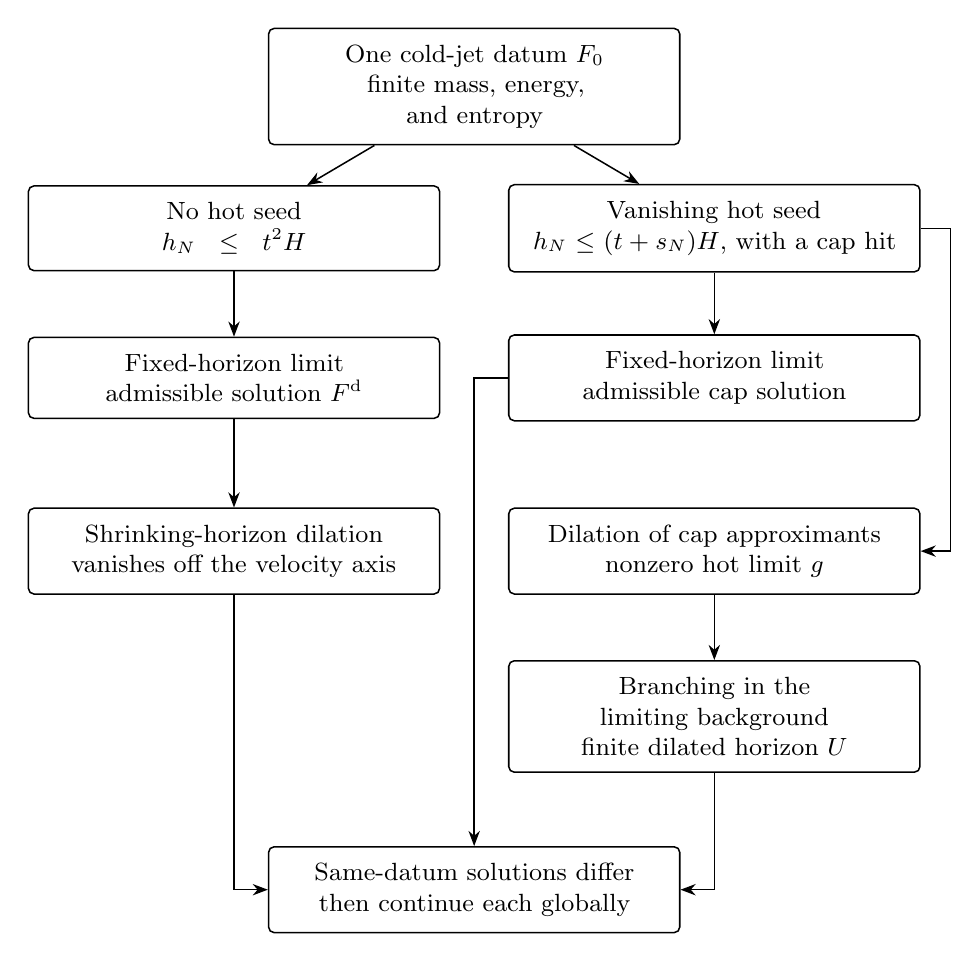
\begin{tikzpicture}[
 box/.style={draw,rounded corners=2pt,align=center,text width=4.8cm,
             inner sep=6pt,font=\small},
 every path/.style={line width=.55pt}, >=Stealth]
\node[box] (datum) at (0,0)
 {One cold-jet datum $F_0$\\finite mass, energy,\\and entropy};
\node[box] (dormant) at (-3.05,-1.8)
 {No hot seed\\$h_N\le t^2H$};
\node[box] (seed) at (3.05,-1.8)
 {Vanishing hot seed\\$h_N\le(t+s_N)H$, with a cap hit};
\node[box] (dl) at (-3.05,-3.7)
 {Fixed-horizon limit\\admissible solution $F^{\mathrm d}$};
\node[box] (sl) at (3.05,-3.7)
 {Fixed-horizon limit\\admissible cap solution};
\node[box] (zero) at (-3.05,-5.9)
 {Shrinking-horizon dilation\\vanishes off the velocity axis};
\node[box] (dilation) at (3.05,-5.9)
 {Dilation of cap approximants\\nonzero hot limit $g$};
\node[box] (growth) at (3.05,-8.0)
 {Branching in the\\limiting background\\finite dilated horizon $U$};
\node[box] (separate) at (0,-10.2)
 {Same-datum solutions differ\\then continue each globally};
\draw[->] (datum) -- (dormant);
\draw[->] (datum) -- (seed);
\draw[->] (dormant) -- (dl);
\draw[->] (seed) -- (sl);
\draw[->] (seed.east) -- (6.05,-1.8) |- (dilation.east);
\draw[->] (dilation) -- (growth);
\draw[->] (dl) -- (zero);
\draw[->] (zero.south) -- (-3.05,-10.2) -- (separate.west);
\draw[->] (sl.west) -- (0,-3.7) -- (separate.north);
\draw[->] (growth.south) -- (3.05,-10.2) -- (separate.east);
\end{tikzpicture}

\caption{Proof structure. At each fixed physical horizon, the two
approximation families yield admissible solutions with the same initial
datum. Separately, cap approximants on shrinking horizons are dilated
about a cap hit. Nonconcentration preserves a nonzero hot limit, and
branching prevents its scale from vanishing relative to the horizon along
the extracted sequence. These facts contradict equality with the dormant
limit, whose corresponding dilation vanishes off the velocity axis.}
\label{fig:proof-route}
\end{figure}

\subsection{Organization}

Section~\ref{sec:framework} gives the full admissibility definition and
the colored equations. Section~\ref{ker:section} establishes uniform
collision-kernel estimates, and Section~\ref{jet:section} constructs the
datum and controls its cold components. Section~\ref{sec:cap} selects
the approximation families; Section~\ref{sec:admissibility} constructs
their fixed-horizon limits and verifies admissibility.
Section~\ref{sec:dilation} identifies the dilated linear equation, and
Section~\ref{nc:section} proves that its hot limit is nonzero.
Section~\ref{sec:branching} excludes an infinite dilated horizon.
Section~\ref{sec:separation} completes the same-datum comparison and
global continuation.

\section{Equation, admissibility, and notation}\label{sec:framework}

The spatial torus \(\T^3=\R^3/\mathbb Z^3\) has volume one, and
\(\Omega=\T^3_x\times\R^3_v\). We write \(x=(y,z)\), with two transverse
coordinates \(y\) and one axial coordinate \(z\), and
\(v=(\bar v,v_3)\). In a periodic lift these coordinates range in
\(\R^2\times\R\). All spatially rescaled limits below are taken in the lift.
We write \(D_t=\partial_t+v\cdot\nabla_x\) for free transport.

For incoming velocities \(v,v_*\) and \(\omega\in S^2\), set
\[
a=(v-v_*)\cdot\omega,\qquad
v'=v-a\omega,\qquad v_*'=v_*+a\omega.
\]
The surface measure on \(S^2\) is its ordinary area measure. We use
\begin{equation}\label{eq:collision}
\begin{split}
Q(F,F)&=Q^+(F,F)-Q^-(F,F),\\
Q^+(F,F)(v)&=\int_{\R^3\times S^2}|a|F(v')F(v_*')\dd v_*\dd\omega,\\
Q^-(F,F)(v)&=F(v)\nu_F(v).
\end{split}
\end{equation}
Arguments \(t,x\), identical in every factor, are suppressed.
The associated symmetric gain is denoted \(P(f,g)\), so that
\(P(F,F)=Q^+(F,F)\). Its symmetry in the hard-sphere normalization is
included in Lemma~\ref{lem:carleman}. The loss frequency is
\begin{equation}\label{eq:frequency}
\nu_f(v)=2\pi\int_{\R^3}|v-w|f(w)\dd w.
\end{equation}
A superscript \(b\) on \(P,\nu,Q\) means that the same factor
\(\ind_{\{|v-v_*|<b\}}\) is inserted into gain and loss.
This cutoff is invariant under elastic collision.

Put
\[
M(v)=(2\pi)^{-3/2}e^{-|v|^2/2},\qquad G=F/M,
\]
and define
\[
\mathcal H_M(F)=\int_\Omega
 \bigl(F\log(F/M)-F+M\bigr)\dd x\dd v.
\]
The entropy dissipation is
\[
\mathcal D(F)=\frac14
\int_{\T^3\times\R^3\times\R^3\times S^2}
|a|\,(F'F_*'-FF_*)\log\frac{F'F_*'}{FF_*}
 \dd x\dd v\dd v_*\dd\omega.
\]
The nonnegative integrand is assigned its lower-semicontinuous
extended value when a factor vanishes. We use \(0|\log0|=0\).

\begin{definition}[Entropy-class solution]\label{def:admissible}
For a nonnegative datum \(F_0\) satisfying
\[
\int_\Omega F_0(1+|v|^2+|\log F_0|)\dd x\dd v<\infty,
\]
an admissible global solution is a nonnegative \(F\) with the following
properties.
\begin{enumerate}[label=\textup{(\roman*)}]
\item \(F\in C_w([0,\infty);L^1(\Omega))\), with \(F(0)=F_0\), where
weak continuity means continuity against every bounded measurable test.
On each bounded time interval,
\(\int_\Omega F(1+|v|^2+|\log F|)\) is uniformly bounded.
\item \(Q^\pm(F,F)/(1+G)\) belong to
\(L^1([0,T]\times\Omega)\) for every finite \(T\).
For every \(\beta\in C^1([0,\infty))\) with \(\beta(0)=0\) and
\(|\beta'(z)|\le C_\beta/(1+z)\), and every smooth test
\(\varphi(t,x,v)\) periodic in \(x\) and compactly supported in
\([0,\infty)\times\R^3_v\),
\[
\begin{split}
&\int_0^\infty\!\!\int_\Omega
 \bigl[M\beta(G)(\partial_t\varphi+v\cdot\nabla_x\varphi)
      +\beta'(G)Q(F,F)\varphi\bigr]\dd x\dd v\dd t\\
&\hspace{2cm}
+\int_\Omega M\beta(F_0/M)\varphi(0,x,v)\dd x\dd v=0 .
\end{split}
\]
\item With \(\rho=\int F\dd v\) and \(j=\int vF\dd v\),
\(\partial_t\rho+\nabla_x\cdot j=0\) distributionally with the initial
density \(\int F_0\dd v\). Total momentum is conserved. For every \(t\ge0\),
\[
\int_\Omega |v|^2F(t)\le\int_\Omega |v|^2F_0,\qquad
\mathcal H_M(F(t))+\int_0^t\mathcal D(F(s))\dd s
 \le\mathcal H_M(F_0).
\]
\end{enumerate}
\end{definition}

The same definition on a finite interval uses tests and traces on that
interval. We use the global existence theory
\cite{DiPernaLions1989,DiPernaLions1991,LevermoreMasmoudi2010} only to
continue solutions already constructed on a short interval. In particular,
we do not require local momentum or local energy conservation as additional
admissibility conditions.

\subsection{A velocity weight and colored components}

Fix \(1<q<2\) and \(m=100\). The weight used throughout is
\begin{equation}\label{eq:weight}
H(v)=e^{-|v|^2}\langle v\rangle^{-m}
       \bigl(1+|\bar v|^{-q}\bigr),\qquad
\langle v\rangle=(1+|v|^2)^{1/2}.
\end{equation}
Its values on the velocity axis can be assigned arbitrarily; all weighted
supremum estimates are essential estimates. It is integrable with every
polynomial velocity weight and lies in \(L^p\) for some \(p>1\).
Write \(\|f\|_H=\esssup_{x,v}|f(x,v)|/H(v)\).

The cold components are \(c_i\), their sum is \(c\), and \(h\) denotes
the hot component. Particles retain a cold label only in collisions
within that label. All other collisions create hot particles. With
\(F=c+h\), this gives
\begin{equation}\label{eq:colored}
\begin{split}
(\D)c_i&=P(c_i,c_i)-c_i\nu_F,\\
(\D)h&=2P(c,h)+P(h,h)+\sum_{i\ne j}P(c_i,c_j)-h\nu_F.
\end{split}
\end{equation}
The sum over \(i\ne j\) is ordered. Summing these equations gives
\((\D)F=Q(F,F)\). This identity also holds with a common collision cutoff.
When labels include periodic copies, the individual functions are defined
in the lift and are covariant under translations; their sums are periodic.

Constants denoted \(C\), with or without subscripts, may depend on the
fixed construction parameters. They never depend on the approximation
index or the shrinking time horizon unless explicitly stated. The
parameters needed for branching growth will be fixed before the final
small geometric and time parameters. Section~\ref{sec:branching} records
the order of choices.

\section{Collision kernels and a velocity majorant}
\label{ker:section}

The construction in the next section uses cold velocity distributions
with arbitrarily small transverse widths. We seek bounds for
$P(c,H)/H$ that remain uniform as those widths tend to zero, together
with a bound for $P(H,H)/H$. The later nonconcentration argument needs
more than bounded total gain: it also needs control of the complete
normalized measure in the cold and hot input velocities. We obtain
both kinds of estimates below.

Write $v=(\bar v,v_3)\in\R^2\times\R$ and set
\[
 W(v)=1+|\bar v|^{-q},\qquad
 H(v)=e^{-|v|^2}\langle v\rangle^{-m}W(v),
 \qquad 1<q<2,\quad m=100,
\]
as in \eqref{eq:weight}. Values on the velocity axis are irrelevant to
all the almost-everywhere estimates below. The function $H$ has every
polynomial moment and belongs to $L^p(\R^3)$ whenever $1\leq p<2/q$.
Indeed, its only local singularity is $|\bar v|^{-q}$ in two dimensions,
and its decay at infinity is Gaussian.

\subsection{The exact Carleman formula}

The hyperplane representation used here is a Carleman formula;
see also \cite[Appendix~C]{GambaPanferovVillani2009}.
We derive its coefficient for the normalization of this paper.

\begin{lemma}[Collision geometry]\label{lem:carleman}
For the normalization in \eqref{eq:collision}, the symmetric bilinear
gain is
\begin{equation}\label{ker:carleman}
 P(c,h)(v)
 =2\int_{\R^3}c(p)\,\dd p
       \int_{\R^3}
       \delta\bigl((v-p)\cdot(\xi-v)\bigr)h(\xi)\,\dd\xi.
\end{equation}
For fixed $p\ne v$, the inner delta denotes surface measure on the
plane $(v-p)\cdot(\xi-v)=0$, divided by $|v-p|$.
For incoming velocities $p,\xi$, the outgoing measure has total mass
$2\pi|p-\xi|$ and is uniform on the sphere with diameter $[p,\xi]$.
Formula~\eqref{ker:carleman} also defines the gain when $c$ is a
nonnegative velocity measure and $h$ is a nonnegative density, whenever
the displayed integral is finite almost everywhere.
\end{lemma}

\begin{proof}
Put $g=p-\xi$. Reflection sends $g$ to
$g-2(g\cdot\omega)\omega$. On either hemisphere of the normal sphere,
the change from the polar angle of $\omega$ to the reflected direction
shows that $|g\cdot\omega|\,\dd\omega$ pushes forward to
$(|g|/4)\,\dd\sigma$. The two hemispheres therefore give
$(|g|/2)\,\dd\sigma$, where $\sigma\in S^2$ is the outgoing relative
direction. Equivalently, for every nonnegative test function $\psi$,
the one-output measure is
\begin{equation}\label{ker:sphere-law}
 \frac{|p-\xi|}{2}\int_{S^2}
 \psi\left(\frac{p+\xi}{2}
                 +\frac{|p-\xi|}{2}\sigma\right)\dd\sigma.
\end{equation}
Its mass is $2\pi|p-\xi|$. The affine map in this integral multiplies
surface area by $|p-\xi|^2/4$, so the density on its image sphere is
$2/|p-\xi|$.

The same sphere is the zero set of
$f(v)=(v-p)\cdot(\xi-v)$. On that sphere,
$|\nabla_v f(v)|=|p-\xi|$. The coarea formula consequently identifies
the measure in \eqref{ker:sphere-law} with $2\delta(f(v))\,\dd v$.
Integration against the two incoming densities and Tonelli's theorem
give \eqref{ker:carleman}. The usual pre/post-collisional change of
variables identifies this incoming-pair expression with the gain in
\eqref{eq:collision}. Coincident incoming velocities have zero
collision rate. The same identities can first be integrated against a
velocity measure $c(\dd p)$, proving the asserted extension.
\end{proof}

The cutoff gain obtained by inserting $\ind_{|p-\xi|<b}$ is bounded by
the uncut gain. Thus all upper estimates in this section also hold for
the collision cutoffs used later.

\subsection{A geometric slice estimate}

For $d>0$, let $\mathcal G_d$ be the centered transverse Gaussian
probability measure with density
\[
 \frac{1}{\pi d^2}e^{-|\bar p|^2/d^2},
\]
and let $\mathcal G_0=\delta_0$. We shall also use the uniform
probability measure $\mathcal U_d$ on $\{\bar p:|\bar p|<d\}$.

\begin{lemma}[Transverse averaging and axial slices]
\label{ker:geometric-slice}
Let $\lambda$ be a probability mixture of the measures
$\mathcal U_d$, $d>0$, and $\delta_0$, and let $\rho$ be any axial
probability measure. No bound on its density or its support is
required. Put $c=\lambda\otimes\rho$. For $R\geq1$, $\bar v\ne0$,
and an interval $I\subset\R$ of length $0<\ell\leq2R$, one has
\begin{align}
 &\frac{1}{W(v)}\int c(\dd p)
   \int_{|\xi-v|\leq R}
    \delta\bigl((v-p)\cdot(\xi-v)\bigr)W(\xi)\,\dd\xi
     \leq C_q R^2,\label{ker:geometric-total}\\
 &\frac{1}{W(v)}\int c(\dd p)
   \int_{\substack{|\xi-v|\leq R\\ \xi_3\in I}}
    \delta\bigl((v-p)\cdot(\xi-v)\bigr)W(\xi)\,\dd\xi
     \leq C_q\bigl(R\ell+R^{q-1}\ell^{2-q}\bigr).
     \label{ker:geometric-interval}
\end{align}
The constants are independent of all transverse widths and of $\rho$.
In particular, these statements hold with $\lambda=\mathcal G_d$ for
every $d\geq0$.
\end{lemma}

\begin{proof}
Set $r=|\bar v|$, $n=\bar v-\bar p$, and $e_n=n/|n|$. Except on a
set of transverse measure zero, $n\ne0$. For fixed $p_3,\xi_3$, the
delta in the transverse variables is line measure divided by $|n|$,
on a line whose signed distance from zero is
\[
 A-B(\xi_3-v_3),\qquad
 A=e_n\cdot\bar v,\quad B=\frac{v_3-p_3}{|n|}.
\]
The regular part of its integral over $|\xi-v|\leq R$ is at most
$2R/|n|$. The singular part is bounded by its integral over the full
line, namely
\begin{equation}\label{ker:line-integral}
 \frac{1}{|n|}\int_{\R}
      \bigl((A-B(\xi_3-v_3))^2+s^2\bigr)^{-q/2}\,\dd s
 =\frac{a_q}{|n|}|A-B(\xi_3-v_3)|^{1-q},
\end{equation}
where $a_q=\int_{\R}(1+s^2)^{-q/2}\,\dd s<\infty$ because $q>1$.
Infinite values on a zero-distance slice are harmless in the
nonnegative iterated integral.

For every interval $J\subset[-R,R]$ of length at most $\ell$,
\begin{equation}\label{ker:scalar-interval}
 \int_J |A-Bx|^{1-q}\,\dd x
 \leq C_q R^{q-1}\ell^{2-q}|A|^{1-q}.
\end{equation}
If $2R|B|\leq|A|$, the integrand is at most
$C_q|A|^{1-q}$, and the assertion follows from $\ell\leq2R$.
Otherwise, integration about the possible root gives an upper bound
$C_q|B|^{1-q}\ell^{2-q}$; since $1-q<0$ and
$|B|>|A|/(2R)$, this proves \eqref{ker:scalar-interval}. When $A=0$
the displayed upper bound is understood in the extended sense.

We next prove
\begin{equation}\label{ker:transverse-expectation}
 \int\frac{1+|e_n\cdot e_{\bar v}|^{1-q}}{|n|}\,
          \lambda(\dd\bar p)\leq\frac{C_q}{r}.
\end{equation}
It suffices to consider a disk of radius $d$. If $d\leq r/2$, then
$|n|\geq r/2$ and $e_n\cdot e_{\bar v}\geq1/3$, which proves the
bound. If $d>r/2$, use polar coordinates for $n$. Its range lies in
$|n|<r+d<3d$. The factor $|n|^{-1}$ cancels the radial Jacobian, while
\[
 \int_0^{2\pi}\bigl(1+|\cos\theta|^{1-q}\bigr)\,\dd\theta<\infty
\]
because $q<2$. Division by the disk area gives $C_q/d\leq2C_q/r$.
The point mass at zero satisfies the same estimate directly.
Finally, the Gaussian is a probability mixture of these disks: for
$d>0$ its mixture density in the disk radius $a$ is
\[
 \frac{2a^3}{d^4}e^{-a^2/d^2}\,\dd a,
\]
whose integral is one. This proves the Gaussian assertion as well.

Integrating \eqref{ker:line-integral} in $\xi_3$, applying
\eqref{ker:scalar-interval}, and then
\eqref{ker:transverse-expectation}, bounds the expression in
\eqref{ker:geometric-interval} by
\[
 C_q R\ell\frac{r^{-1}}{1+r^{-q}}
 +C_qR^{q-1}\ell^{2-q}\frac{r^{-q}}{1+r^{-q}}.
\]
Both fractions are bounded for $q>1$. These bounds are independent of
$p_3$, so integration against the arbitrary probability $\rho$
preserves them. Taking the entire axial range of length $2R$ also
gives \eqref{ker:geometric-total}.
\end{proof}

\subsection{Sheets and normalized kernel measures}

\begin{definition}[Uniform sheet class]\label{ker:sheet-class}
Fix $L\geq1$. An elementary sheet in $\mathcal S_L$ is a product
probability measure
\begin{equation}\label{ker:sheet-definition}
 c(\dd p)=\mathcal G_d(\dd\bar p)\rho(\dd p_3),\qquad
 0\leq d\leq\tfrac18,\qquad
 \int_{\R}e^{8a^2}\rho(\dd a)\leq L.
\end{equation}
We also allow probability mixtures of elementary sheets. An upper
bound by a sheet with amplitude $A_0$ means domination as measures by
$A_0$ times such a mixture.
\end{definition}

Every axial probability supported in $[-A,A]$ satisfies this
definition with $L=e^{8A^2}$. In particular, axial atoms and limits of
arbitrarily narrow axial densities are permitted. The exponential
moment is used only to remove large axial velocities, and imposes no
axial regularity.

For such a sheet and $\bar v\ne0$, define its normalized kernel by
\begin{equation}\label{ker:normalized-kernel}
 \mathcal K_c(v;\dd p\,\dd\xi)
 =2\,c(\dd p)\,
       \delta\bigl((v-p)\cdot(\xi-v)\bigr)
       \frac{H(\xi)}{H(v)}\,\dd\xi.
\end{equation}
The total mass is $P(c,H)(v)/H(v)$. Kernel restrictions always refer
to this complete measure, including the ratio $H(\xi)/H(v)$.

\begin{lemma}[Uniform sheet gain bound]\label{lem:sheet-bound}
For every $L<\infty$ there is $C_{q,m,L}<\infty$ such that
\begin{equation}\label{ker:sheet-gain}
 P(c,H)(v)\leq C_{q,m,L}H(v)
 \quad\hbox{for almost every }v,
 \qquad c\in\mathcal S_L.
\end{equation}
More quantitatively, for $R\geq1$,
\begin{equation}\label{ker:shell-tail}
 \mathcal K_c\bigl(v;
      R<|p|+|\xi-v|\leq2R\bigr)
 \leq C_{q,m,L}R^2e^{-cR^2},
\end{equation}
where $c>0$ is an absolute constant. The same conclusions, multiplied
by $A_0$, hold under sheet domination with amplitude $A_0$.
\end{lemma}

\begin{proof}
By positivity it suffices to treat an elementary sheet. Put
$k=\xi-v$ and $w=p+k$. On the collision plane,
\begin{equation}\label{ker:energy-factor}
 |p|^2+|\xi|^2=|v|^2+|w|^2,
 \qquad
 \frac{H(\xi)}{H(v)}
 =e^{|p|^2-|w|^2}
    \frac{\langle v\rangle^m}{\langle\xi\rangle^m}
    \frac{W(\xi)}{W(v)}.
\end{equation}
The same identity implies
$\langle v\rangle\leq\langle p\rangle\langle\xi\rangle$.
Since $\langle p\rangle^m\leq C_m e^{|p|^2}$, the kernel is bounded
by
\begin{equation}\label{ker:tilted-kernel}
 C_m e^{2|p|^2}c(\dd p)\,
 e^{-|w|^2}\delta\bigl((v-p)\cdot k\bigr)
       \frac{W(v+k)}{W(v)}\,\dd k.
\end{equation}

The tilted cold measure retains a product majorant. For $0<d\leq1/8$,
\begin{equation}\label{ker:transverse-tilt}
 e^{2|\bar p|^2}\mathcal G_d(\dd\bar p)
 \leq4e^{-46|\bar p|^2}\mathcal G_{2d}(\dd\bar p).
\end{equation}
This follows by dividing the two Gaussian densities: their ratio is
$4\exp[-(3/(4d^2)-2)|\bar p|^2]$, and
$3/(4d^2)-2\geq46$. The assertion at $d=0$ has the evident
interpretation. The axial tilted measure
$\widetilde\rho(\dd a)=e^{2a^2}\rho(\dd a)$ has mass at most $L$,
and satisfies
\begin{equation}\label{ker:axial-tilt-tail}
 \widetilde\rho\{|a|>u\}\leq Le^{-6u^2},\qquad u\geq0.
\end{equation}
Consequently $e^{2|p|^2}c(\dd p)$ is bounded by $4L$ times a product
of a centered transverse Gaussian and an axial probability. Moreover,
its restriction to $|p|>u$ is bounded by
$CLe^{-cu^2}$ times a sum of at most two such product probabilities.
To see the last assertion, split into $|\bar p|>u/\sqrt2$ and
$|p_3|>u/\sqrt2$, and apply
\eqref{ker:transverse-tilt} and \eqref{ker:axial-tilt-tail},
respectively. The axial probabilities obtained by normalization may
have large support; Lemma~\ref{ker:geometric-slice} permits this.

On the shell in \eqref{ker:shell-tail}, either $|p|>R/4$ or
$|w|>R/2$, because $|p|+|k|\leq2|p|+|w|$. In the first case the
preceding tilted-measure tail contributes $CLe^{-cR^2}$. In the
second case $e^{-|w|^2}\leq e^{-R^2/4}$. In either case the remaining
integral has $|k|\leq2R$ and is bounded by $C_qR^2$ using
Lemma~\ref{ker:geometric-slice}. This proves
\eqref{ker:shell-tail}. The base region $|p|+|k|\leq2$ is bounded
by the same geometric lemma and the total tilted mass. Summing the
dyadic shells proves \eqref{ker:sheet-gain} and also the finiteness
of \eqref{ker:normalized-kernel}.
\end{proof}

The sheet gain bound controls total normalized mass. We next control
its velocity tails and its behavior as the outgoing velocity approaches
the axis. The key distinction is that the hot input can concentrate
transversely on the axis while its axial marginal remains uniformly
non-atomic.

\begin{lemma}[Uniform tightness and axis estimates]
\label{lem:kernel-tightness}
Fix $L<\infty$. The following conclusions hold uniformly for
$c\in\mathcal S_L$ and for outgoing velocities off the axis.
\begin{enumerate}[label=\textup{(\roman*)}]
\item The tails in $|p|+|\xi-v|$ are uniformly negligible:
\begin{equation}\label{ker:uniform-tail}
 \lim_{R\to\infty}\sup_{c\in\mathcal S_L}\esssup_v
 \mathcal K_c(v;|p|+|\xi-v|>R)=0.
\end{equation}
Also,
\begin{equation}\label{ker:large-output}
 \lim_{M\to\infty}\sup_{c\in\mathcal S_L}
 \esssup_{|v|>M}\mathcal K_c(v;\R^3\times\R^3)=0.
\end{equation}
\item For every fixed $M,\delta>0$,
\begin{align}
 &\lim_{\varepsilon\downarrow0}
 \sup_{c\in\mathcal S_L}
 \esssup_{\substack{|v|\leq M\\0<|\bar v|\leq\varepsilon}}
 \mathcal K_c(v;|\bar\xi|\geq\delta)=0,
 \label{ker:axis-input}\\
 &\lim_{\varepsilon\downarrow0}
 \sup_{c\in\mathcal S_L}
 \esssup_{\substack{|v|\leq M\\0<|\bar v|\leq\varepsilon}}
 \mathcal K_c(v;|v_3-p_3|\geq\delta)=0.
 \label{ker:axis-mismatch}
\end{align}
\item The axial input marginals are uniformly non-atomic. More
precisely, for each $R\geq1$ and each interval $I$ of length
$0<\ell\leq1$,
\begin{equation}\label{ker:axial-interval}
 \mathcal K_c(v;|p|+|\xi-v|\leq R,\ \xi_3\in I)
 \leq C_{q,m,L,R}\bigl(\ell+\ell^{2-q}\bigr).
\end{equation}
In combination with \eqref{ker:uniform-tail}, this gives
\begin{equation}\label{ker:axial-modulus}
 \lim_{\ell\downarrow0}\sup_{c\in\mathcal S_L}\esssup_v
 \sup_{|I|\leq\ell}\mathcal K_c(v;\xi_3\in I)=0.
\end{equation}
\item Let $\mathcal S_L(\varepsilon)$ denote the subclass whose
elementary transverse widths are at most $\varepsilon$. For every
$M<\infty$ and $r_0>0$,
\begin{equation}\label{ker:off-axis-small-input}
 \lim_{\delta\downarrow0}\limsup_{\varepsilon\downarrow0}
 \sup_{c\in\mathcal S_L(\varepsilon)}
 \esssup_{\substack{|v|\leq M\\|\bar v|\geq r_0}}
 \mathcal K_c(v;|\bar\xi|<\delta)=0.
\end{equation}
\end{enumerate}
All these conclusions hold under uniformly bounded sheet amplitudes.
\end{lemma}

\begin{proof}
The dyadic estimate \eqref{ker:shell-tail} proves
\eqref{ker:uniform-tail}. We may consequently work on
$|p|+|k|\leq R$ and remove that restriction at the end of each
argument. On this region the exponential and polynomial factors in
\eqref{ker:energy-factor} are bounded by a constant depending on $R$.

For \eqref{ker:large-output}, if $|\bar v|>2R+1$, then
$|\bar v-\bar p|\geq|\bar v|/2$ and
$|\bar\xi|\geq|\bar v|-R$. The transverse line estimate, followed
by the axial integration over a length at most $2R$, gives
$C_R/|\bar v|$. If $|v_3|>2R+1$, integrate the delta in $\xi_3$
instead. Its divisor is $|v_3-p_3|\geq|v_3|/2$, and
\begin{equation}\label{ker:disk-singularity}
 \sup_{a\in\R^2}\int_{|\zeta-a|\leq R}
       (1+|\zeta|^{-q})\,\dd\zeta
 \leq C_q(R^2+R^{2-q}).
\end{equation}
For completeness, if $|a|\leq2R$ the disk is contained in the disk
of radius $3R$ about zero; if $|a|>2R$, then $|\zeta|>|a|/2>R$ on
the disk, giving the same bound. We obtain $C_R/|v_3|$. At least one
of the two outgoing components becomes large with $|v|$, proving
\eqref{ker:large-output}.

For \eqref{ker:axis-input}, on $|\bar\xi|\geq\delta$ the factor
$W(\xi)$ is bounded by $1+\delta^{-q}$. The regular line estimate
and \eqref{ker:transverse-expectation} therefore give
\[
 C_{R,\delta}\frac{|\bar v|^{-1}}{1+|\bar v|^{-q}}
 \leq C_{R,\delta}|\bar v|^{q-1}
 \qquad(0<|\bar v|\leq1).
\]
For \eqref{ker:axis-mismatch}, integrate in $\xi_3$ first, using
$|v_3-p_3|^{-1}\leq\delta^{-1}$ and
\eqref{ker:disk-singularity}. The bound is
$C_{R,\delta}/W(v)\leq C_{R,\delta}|\bar v|^q$.
These are uniform in the axial law. For
\eqref{ker:axial-interval}, discard the bounded exponential and
polynomial factors and apply
\eqref{ker:geometric-interval}. This also proves
\eqref{ker:axial-modulus} after the tail removal.

It remains to prove \eqref{ker:off-axis-small-input}. Fix the
truncation radius $R$. The part $|\bar p|>r_0/4$ is uniformly
negligible as the transverse widths tend to zero. Indeed,
\[
 \ind_{|\bar p|>r_0/4}\mathcal G_d(\dd\bar p)
 \leq2e^{-r_0^2/(32d^2)}\mathcal G_{\sqrt2d}(\dd\bar p),
\]
and Lemma~\ref{lem:sheet-bound} applies to the wider Gaussian for
all sufficiently small $d$. Now retain $|\bar p|\leq r_0/4$.
With the notation of Lemma~\ref{ker:geometric-slice},
\[
 |n|\geq\tfrac34r_0,\qquad
 A=\frac{(\bar v-\bar p)\cdot\bar v}{|\bar v-\bar p|}
     \geq\tfrac35r_0.
\]
If $|v_3-p_3|\leq r_0^2/(8R)$, then for
$|\xi_3-v_3|\leq R$,
\[
 |B(\xi_3-v_3)|\leq\tfrac16r_0.
\]
The transverse collision line stays at distance greater than
$r_0/3$ from zero, and cannot meet $|\bar\xi|<\delta$ when
$\delta<r_0/3$. In the complementary case,
$|v_3-p_3|^{-1}\leq8R/r_0^2$. Integrating first in $\xi_3$ bounds
the small-input contribution by
\[
 C_{R,r_0}\int_{|\bar\xi|<\delta}
               (1+|\bar\xi|^{-q})\,\dd\bar\xi
 \leq C_{R,r_0}(\delta^2+\delta^{2-q}).
\]
First let the widths tend to zero, then $\delta$ tend to zero, and
finally remove the truncation. This proves the last assertion.
\end{proof}

\subsection{Gaussian parameter laws and compressed axial maps}

The next formulation records the uniformity needed when a cold
profile is parameterized before its axial change of variables.

\begin{lemma}[Gaussian parameter tails]
\label{ker:parameter-sheets}
Let a measure in parameters $w=(\bar w,w_3)\in\R^2\times\R$ have
density $j$ satisfying
\[
 0\leq j(w)\leq C_0\pi^{-3/2}e^{-|w|^2}.
\]
Let its velocity image be given by
\begin{equation}\label{ker:parameter-map}
 \bar p=d\bar w,\qquad p_3=\Phi(w_3),\qquad
 0\leq d\leq\tfrac1{16},\qquad
 |\Phi(a)|\leq A+\delta|a|,\quad0\leq\delta\leq\tfrac1{16},
\end{equation}
where $\Phi$ is merely measurable. The image measure is dominated
by $C_0$ times a sheet in $\mathcal S_{L_A}$, with $L_A$ depending
only on $A$. Its gain satisfies Lemma~\ref{lem:sheet-bound} with a
constant depending only on $q,m,A,C_0$.

If $c_{>B}$ is the image of the restricted parameter measure
$\ind_{|w|>B}j(w)\,\dd w$, then
\begin{equation}\label{ker:parameter-tail}
 \esssup_v\frac{P(c_{>B},H)(v)}{H(v)}
 \leq C_{q,m,A,C_0}e^{-B^2/2},\qquad B\geq0.
\end{equation}
Thus parameter truncations are valid in the normalized collision
measure, even when $\Phi$ compresses intervals or has atoms in its
image law. Probability mixtures of measurable families with common
$q,m,A,C_0$ and the width bounds in \eqref{ker:parameter-map} preserve
these assertions. More generally, a positive mixing measure of total
mass $B_0<\infty$ multiplies the domination amplitude and quantitative
upper bounds by $B_0$; the sheet parameter $L_A$ is unchanged.
For \eqref{ker:parameter-tail}, impose the restriction $|w|>B$ in
each component before mixing. Additional measurable masks taking
values in $[0,1]$ preserve the assertions.
\end{lemma}

\begin{proof}
The Gaussian majorant is a product measure. Its transverse image is
$\mathcal G_d$, and its axial image is the probability
$\rho=\Phi_*(\pi^{-1/2}e^{-a^2}\,\dd a)$. There is no need to
differentiate or invert $\Phi$. From \eqref{ker:parameter-map},
\[
 e^{8|\Phi(a)|^2}\leq e^{16A^2}e^{16\delta^2a^2}.
\]
Even under the wider axial probability
$(2\pi)^{-1/2}e^{-a^2/2}\,\dd a$, the integral of the right side
is
\[
 e^{16A^2}(1-32\delta^2)^{-1/2}\leq2e^{16A^2}.
\]
We may therefore take $L_A=2e^{16A^2}$ for both the original and
the wider parameter laws. The original image has the required
sheet domination.

On the parameter tail,
\[
 \ind_{|w|>B}e^{-|w|^2}
 \leq e^{-B^2/2}e^{-|w|^2/2}.
\]
After normalization the right side is $2^{3/2}e^{-B^2/2}$ times a
Gaussian probability with parameter widths enlarged by $\sqrt2$.
Its transverse velocity width is at most $\sqrt2/16<1/8$, and
its axial image has the exponential moment just proved.
Lemma~\ref{lem:sheet-bound} applied to this dominating image gives
\eqref{ker:parameter-tail}.

For a probability mixture, mix the dominating sheets just constructed;
this is again a member of $\mathcal S_{L_A}$. If the mixing measure
has mass $B_0>0$, normalize it by $B_0$ and retain that factor in
the domination amplitude. If $B_0=0$, the mixed image is zero.
The same argument applied to the wider Gaussian majorants of the
component tails proves the asserted factor in
\eqref{ker:parameter-tail}. Thus the estimates are uniform over
families of mixtures whose masses $B_0$ have a common finite bound
independent of the tail cutoff. Masks taking values in $[0,1]$ only
decrease the measures, whether imposed before or after the pushforward.
\end{proof}

For example, suppose an axial velocity is determined by
$p_3=a(z-tp_3)+d w_3$, where $a$ is nondecreasing, and $u$ solves
$u=a(z-tu)$. The function $p\mapsto p-a(z-tp)$ is increasing with
inverse Lipschitz constant at most one. Hence
\begin{equation}\label{ker:compressed-displacement}
 |p_3-u|\leq d|w_3|.
\end{equation}
If $|u|\leq A$, Lemma~\ref{ker:parameter-sheets} applies. A large
Jacobian compression of the axial law does not affect its constants.
Gaussian majorants with any fixed positive exponent in place of one
are covered by a fixed rescaling of the parameters and a corresponding
decrease of the upper bounds on the physical widths.

\subsection{The hot--hot gain}

\begin{lemma}[Quadratic gain bound]\label{lem:hot-bound}
There is a constant $C_{q,m}$ such that
\begin{equation}\label{ker:hot-gain}
 P(H,H)\leq C_{q,m}H
 \quad\hbox{almost everywhere}.
\end{equation}
In fact the proof below works for every $m>5$.
\end{lemma}

\begin{proof}
The integrand is symmetric in $p,\xi$. On the collision plane,
$|v|^2\leq|p|^2+|\xi|^2$, so at least one incoming speed is at
least $|v|/2$. It suffices, at a factor of two, to retain
$|\xi|\geq|v|/2$. Formula~\eqref{ker:energy-factor} now gives
\begin{align}
 \frac{P(H,H)(v)}{H(v)}
 &\leq C_m\int_{|\xi|\geq|v|/2}
 \delta\bigl((v-p)\cdot(\xi-v)\bigr)
 e^{-|p+\xi-v|^2}\langle p\rangle^{-m}
 \frac{W(p)W(\xi)}{W(v)}\,\dd p\,\dd\xi,
 \label{ker:hot-reduced}
\end{align}
because $\langle v\rangle^m/\langle\xi\rangle^m\leq2^m$.

Again write $k=\xi-v$ and $w=p+k$. On
$R<|p|+|k|\leq2R$, $R\geq1$, either $|p|>R/4$ or $|w|>R/2$.
Consequently
\begin{equation}\label{ker:hot-shell-weight}
 \langle p\rangle^{-m}e^{-|w|^2}
 \leq C_mR^{-m}e^{-|w|^2/2}.
\end{equation}
In the second alternative this uses the finite supremum of
$s^m e^{-s^2/2}$; in the first it follows directly from the
polynomial factor.

The measure $W(p)\ind_{|p|\leq2R}\,\dd p$ is dominated by
\[
 \bigl(1+|\bar p|^{-q}\bigr)
 \ind_{|\bar p|\leq2R}\,\dd\bar p
 \ \otimes\ \ind_{|p_3|\leq2R}\,\dd p_3.
\]
Its transverse factor is a positive mixture of centered disks.
Indeed, for $D>0$,
\[
 |\bar p|^{-q}\ind_{|\bar p|\leq D}
 =D^{-q}\ind_{|\bar p|\leq D}
   +q\int_0^D a^{-q-1}\ind_{|\bar p|\leq a}\,\dd a
\]
almost everywhere. Upon normalizing the disks, the mixture has
total mass
$\pi D^2+2\pi D^{2-q}/(2-q)$. The axial factor has mass $4R$.
For $D=2R$ the resulting product mixture therefore has total mass
at most $C_qR^3$.

Discard $e^{-|w|^2/2}$ and the incoming-speed restriction in
\eqref{ker:hot-reduced}. Apply
Lemma~\ref{ker:geometric-slice} to each normalized product in this
mixture, with $|k|\leq2R$. In conjunction with
\eqref{ker:hot-shell-weight}, this yields the shell estimate
\begin{equation}\label{ker:hot-shell}
 \frac{P(H,H)(v)}{H(v)}\bigg|_{R<|p|+|\xi-v|\leq2R}
 \leq C_{q,m}R^{5-m}.
\end{equation}
The notation on the left denotes the restricted nonnegative
integral from \eqref{ker:hot-reduced}, including its fixed symmetry
factor. The base region is bounded by the same disk-mixture
argument with $R=1$. Summation over dyadic $R$ proves the result
for $m>5$.
\end{proof}

\begin{remark}[A sharp axial endpoint]\label{ker:matching-axis}
A single normalized gain need not become small as the outgoing
velocity approaches the axis. Take $c=\delta_{(0,0,u)}$ and
$v_\varepsilon=(\varepsilon,0,u)$. The collision plane is
$\xi_1=\varepsilon$, and
\[
 \frac{P(c,H)(v_\varepsilon)}{H(v_\varepsilon)}
 =\frac{2}{\varepsilon H(v_\varepsilon)}
      \int_{\R^2}H(\varepsilon,y,z)\,\dd y\,\dd z.
\]
The regular part of $W(\varepsilon,y,z)$ contributes
$O(\varepsilon^{q-1})$. In its singular part substitute
$y=\varepsilon s$. Dominated convergence, with dominating function
$(1+s^2)^{-q/2}e^{-z^2}\langle z\rangle^{-m}$, gives
\[
 \lim_{\varepsilon\downarrow0}
 \frac{P(c,H)(v_\varepsilon)}{H(v_\varepsilon)}
 =2a_q e^{u^2}\langle u\rangle^m
        \int_{\R}e^{-z^2}\langle z\rangle^{-m}\,\dd z>0.
\]
The corresponding axial input marginal converges to the absolutely
continuous measure
\[
2a_q e^{u^2}\langle u\rangle^m
 e^{-z^2}\langle z\rangle^{-m}\,\dd z.
\]
Thus transverse concentration is compatible with the uniform axial
interval estimate. This is the reason for using two successive gains
in the axial part of the later nonconcentration argument.
\end{remark}

\section{Cold jets and uniform color estimates}
\label{jet:section}

We construct the common finite-entropy datum and bound each cold color
by its free transport plus a small Maxwellian remainder. Narrow velocity
profiles control self-collisions, while spatial gaps make collisions
between distinct colors small. These estimates supply the cold density
bound and the mixed-cold source bound used to select the hot caps in
Section~\ref{sec:cap}.

The estimates in this section hold for every fixed choice
\[
 K\ge1,\qquad 0<\eta\le\log2,\qquad
 0<\alpha\le\tfrac14,\qquad 0<\gamma\le1.
\]
These four parameters will subsequently be fixed by the growth argument.
Here we choose the geometric and thermal parameters after them.
To keep the later shortening of the time interval separate from the
estimates, fix the preliminary bounds
\begin{equation}
 \overline s=\tfrac18,\qquad \overline T=\tfrac1{32},
 \qquad 0<s_0\le\overline s,\qquad 0<T_0\le\overline T .
 \label{jet:preliminary}
\end{equation}
All estimates proved below hold on the preliminary interval
\([0,\overline T]\).  Their constants do not change when \(T_0\) is
subsequently decreased.  They may depend on the fixed parameters and on
the fixed function \(J\), but never on the number of retained annuli,
the collision cutoff, or the size of the hot component.

\subsection{The geometry and the datum}

Put
\[
 s_j=s_0e^{-j\eta},\qquad p_j=s_j^2,\qquad
 c_\eta=\frac{e^\eta-1}{16},\qquad
 \delta_j=\frac{c_\eta}{4}s_j^2,\qquad j\ge1.
\]
For \(s=s_j\), define the annular core and the two stripe patterns by
\begin{align*}
 A_j&=\{y\in\R^2:
       s_j+c_\eta p_j<|y|<e^\eta s_j-c_\eta p_j\},\\
 P_j^+&=\bigcup_{k\in\mathbb Z}
       \{y:kp_j<y_1<(k+\tfrac14)p_j\},\\
 P_j^-&=\bigcup_{k\in\mathbb Z}
       \{y:(k+\tfrac12)p_j<y_1<(k+\tfrac34)p_j\},\\
 E_j^\sigma&=A_j\cap P_j^\sigma,\qquad \sigma\in\{-1,+1\}.
\end{align*}
Each stripe pattern has period \(p_j\) and fraction
\(\theta=1/4\).  This is a statement about the periodic pattern:
intersecting it with the annulus need not preserve the fraction
exactly.  We retain the original sets \(E_j^\sigma\) in the datum.

Let
\[
 \widehat E_j^\sigma
   =\{y:\dist(y,E_j^\sigma)\le\delta_j\},
 \qquad a=\tfrac18,\qquad b_{\mathrm{sp}}=\tfrac1{16}.
\]
For a label \(i=(j,\sigma,n)\), \(n=(\bar n,n_3)\in\mathbb Z^3\), set
\begin{equation}
 \mathcal O_i(t)=
 (\widehat E_j^\sigma+\bar n)
 \times[n_3-a-2t-b_{\mathrm{sp}},
        n_3+a+2t+b_{\mathrm{sp}}].
 \label{jet:enlargements}
\end{equation}
These enlargements will only localize upper bounds; they will not
replace the stripe masks when their average is computed.

\begin{lemma}[Disjoint enlargements]
\label{jet:geometry}
For \(0\le t\le\overline T\), the sets \(\mathcal O_i(t)\) are
pairwise disjoint.  Moreover,
\[
 \widehat E_j^\sigma\subset
 \{s_j<|y|<e^\eta s_j\}\subset B(0,s_0).
\]
At each point of the periodic lift there is therefore at most one
label whose enlargement contains that point.
\end{lemma}

\begin{proof}
Opposite stripe patterns at the same scale have distance at least
\(p_j/4\), whereas \(2\delta_j=c_\eta p_j/2<p_j/4\).
The radial gap between the cores for the adjacent scales \(s_j\)
and \(s_{j+1}\) is
\[
 c_\eta(p_j+p_{j+1})
   >\delta_j+\delta_{j+1}.
\]
The gaps between nonadjacent cores are larger.  Enlarging by
\(\delta_j<c_\eta p_j\) still leaves the \(j\)-th set inside its
original open annulus.  This proves disjointness of all the
untranslated transverse enlargements.  They lie in \(B(0,s_0)\),
so their distinct integer translates are disjoint as well.
Finally,
\[
 a+2\overline T+b_{\mathrm{sp}}=\tfrac14.
\]
The axial intervals belonging to distinct integers \(n_3\) are
disjoint.  These two observations prove the assertion for the
products in \eqref{jet:enlargements}.
\end{proof}

Fix a nonnegative smooth probability density \(J\), supported in the
unit ball of \(\R^3\).  Write
\[
 S(\ell)=\operatorname{sech}^2\ell,\qquad
 a_s^\sigma(z)=\sigma+\alpha\tanh(\gamma z/s),
 \qquad d_s=d_0s^{10}.
\]
The positive parameter \(d_0\le1\) will be decreased below finitely
many times.  In particular, we require that
\begin{equation}
 d_0\overline s^{10}\le\tfrac1{64},\qquad
 \overline T d_0\overline s^8\le c_\eta/8 .
 \label{jet:thermal-preliminary}
\end{equation}
The width \(1/64\), including the fixed Gaussian widenings used
below, lies within the range of Lemma~\ref{lem:sheet-bound}.
For \(i=(j,\sigma,n)\), with \(s=s_j\), define on the lift
\[
 c_i^0(x,v)=
 \ind_{E_j^\sigma}(y-\bar n)\ind_{(-a,a)}(z-n_3)
 \frac K s S\!\left(\frac{\gamma(z-n_3)}s\right)d_s^{-3}
 J\!\left(\frac{v-a_s^\sigma(z-n_3)e_3}{d_s}\right).
\]
The periodic datum is
\begin{equation}
 F_0(x,v)=\sum_{j\ge1}\sum_{\sigma=\pm1}
                 \sum_{n\in\mathbb Z^3}c_{(j,\sigma,n)}^0(x,v).
 \label{eq:datum}
\end{equation}
At a given spatial point at most one summand is nonzero.  Integer
translations permute the labels, so the sum is periodic.

\begin{lemma}[Integrability of the datum]
\label{lem:datum}
The datum \eqref{eq:datum} satisfies
\[
 \int_\Omega F_0(1+|v|^2+|\log F_0|)\,\dd x\,\dd v<\infty .
\]
Its truncations \(F_0^{(N)}\), retaining \(j\le N\), converge to
\(F_0\) in mass, energy, and relative entropy.
In addition, if \(\chi\ge0\) is a fixed bounded smooth compactly
supported function of \((x,v)\), periodized after replacing \(x\)
by \(x/s_N\), and \(0\le\lambda_N\le L_0<\infty\), then
\[
 F_0^{(N)}+\lambda_Ns_N\chi(x/s_N,v)
\]
has the same limiting mass, energy, and relative entropy as \(F_0\).
For the last assertion \(s_0\) may be decreased so that distinct
periodic copies of the spatial support of the seed are disjoint.
\end{lemma}

\begin{proof}
Integration over one period and summation over integer copies equal
integration of each unshifted prototype over \(\R^3_x\).
The transverse area of \(E_j^\sigma\) is at most \(C_\eta s_j^2\),
and
\[
 \int_{-a}^a S(\gamma z/s)\,\dd z
 \le \frac s\gamma\int_\R S(\ell)\,\dd\ell
 =\frac{2s}{\gamma}.
\]
The velocity factor integrates to one.  Thus the mass of each
annular sign prototype is at most \(Cs^2\).
Its velocities satisfy
\[
 |v|\le1+\alpha+d_s<2,
\]
which gives the same bound for its energy.

On the set where the density is positive, decompose its logarithm
into the three terms
\[
 \log((K/s)d_s^{-3}),\qquad
 \log S(\gamma z/s),\qquad \log J(w).
\]
The first has absolute value at most \(C(1+|\log s|)\).
The second is integrable against its own weight since
\[
 \int_\R S(\ell)|\log S(\ell)|\,\dd\ell<\infty:
\]
on \(|\ell|\ge1\), its integrand is bounded by
\(C(1+|\ell|)e^{-2|\ell|}\), and on a bounded interval it is bounded.
Also \(\int J|\log J|<\infty\), because \(J\) is bounded and
compactly supported and \(r|\log r|\) is bounded for \(0\le r\le1\).
Consequently the absolute entropy of an annular sign prototype is
at most
\[
 Cs^2(1+|\log s|).
\]
The sums of these bounds over the geometric scales converge.
Since the spatial supports of the prototypes are disjoint modulo
periodicity, the same estimates prove convergence of the truncated
mass, energy, and absolute entropy.  As \(-\log M\) is a constant
plus \(|v|^2/2\), they prove relative entropy convergence as well.

For the seed \(h_N^0=\lambda_Ns_N\chi(x/s_N,v)\), a change of spatial
variables gives
\[
 \int h_N^0(1+|v|^2)\le Cs_N^4,\qquad
 \int h_N^0|\log h_N^0|
       \le Cs_N^4(1+|\log s_N|).
\]
The constants are uniform in \(\lambda_N\in[0,L_0]\), including
\(\lambda_N=0\), since \(\lambda|\log\lambda|\) is bounded on
bounded intervals.
It remains to check overlap with the cold datum.  At every point
\[
 0\le F_0^{(N)}\le C s_N^{-31}.
\]
For \(f,b\ge0\), integration of \(1+\log(f+r)\) over \(0<r<b\)
gives, with the convention at \(b=0\),
\[
 |(f+b)\log(f+b)-f\log f|
 \le b\{2+\log^+(f+b)\}+b|\log b|.
\]
Indeed the positive part of the logarithm is bounded by
\(\log^+(f+b)\), and
\(\int_0^b\log^-(f+r)\,\dd r
 \le\int_0^b\log^-r\,\dd r\le b(1+|\log b|)\).
On the seed support,
\(\log^+(F_0^{(N)}+h_N^0)\le C(1+|\log s_N|)\).
The entropy perturbation is therefore
\(O(s_N^4(1+|\log s_N|))\).  The mass and Maxwellian-reference terms
are controlled by the seed's mass and energy estimates.  This
proves the last assertion.
\end{proof}

\subsection{A transported Maxwellian barrier}

For a fixed scale and sign, the equation
\begin{equation}
 u_s^\sigma(t,z)=a_s^\sigma(z-tu_s^\sigma(t,z))
 \label{jet:scalar-flow}
\end{equation}
defines \(u_s^\sigma\) for all \(t\ge0,z\in\R\).  Indeed
\(\tau\mapsto\tau+t a_s^\sigma(\tau)\) is strictly increasing,
has derivative at least one, and maps \(\R\) onto \(\R\).
In particular, \(|u_s^\sigma|\le1+\alpha\).
For label \(i=(j,\sigma,n)\), abbreviate
\[
 u_i(t,z)=u_{s_j}^\sigma(t,z-n_3),\quad
 \tau_i=z-n_3-tu_i(t,z),\quad w_i=v-u_i(t,z)e_3,
\]
and set
\[
 D_{y,i}=\dist(y-\bar n,E_j^\sigma),\qquad
 D_{z,i}=\dist(\tau_i,[-a,a]).
\]
Choose \(c_{\mathrm{sp}}=1/8\) and a fixed sufficiently large
\(C_m\), depending only on \(J\), and define, for \(t>0\),
\begin{equation}
 m_i(t,x,v)=
 C_m\frac K{s_j}d_{s_j}^{-3} e^t
 \exp\left[-\frac{(2-t)|w_i|^2}{d_{s_j}^2}
 -\frac{c_{\mathrm{sp}}(D_{y,i}^2+D_{z,i}^2)}
              {d_{s_j}^2t}\right].
 \label{jet:majorant}
\end{equation}
Its trace at \(t=0\) is defined by the limit along free
characteristics.  Boundary values of the spatial masks are
irrelevant.  Denote the free transport of the \(i\)-th initial
color by
\[
 f_i(t,x,v)=c_i^0(x-tv,v).
\]

\begin{lemma}[Barrier identities]
\label{jet:barrier}
The constant \(C_m\) can be chosen so that \(f_i\le m_i\) on
\([0,\overline T]\), uniformly in the label.  Moreover, almost
everywhere along every free characteristic,
\begin{equation}
 \D m_i\ge
 \left(1+\tfrac78 |w_i|^2/d_{s_j}^2\right)m_i .
 \label{jet:barrier-derivative}
\end{equation}
There is a constant \(C_\nu\), independent of the label, such that
\begin{equation}
 P(m_i,m_i)=m_i\nu_{m_i},\qquad
 \nu_{m_i}(v)\le C_\nu\frac K{s_j}(d_{s_j}+|w_i|).
 \label{jet:barrier-collision}
\end{equation}
Every free core remains in its own spatial enlargement:
\[
 f_i(t,x,v)>0\quad\Longrightarrow\quad x\in\mathcal O_i(t).
\]
\end{lemma}

\begin{proof}
Suppress the indices, write \(d=d_s\), and put
\(A=(a_s^\sigma)'(\tau)\ge0\).  Implicit differentiation gives
\begin{equation}
 u_z=\frac A{1+tA}\ge0,\qquad
 u_t=-u u_z,\qquad
 \D u=(v_3-u)u_z,\qquad
 \D\tau=\frac{v_3-u}{1+tA}.
 \label{jet:flow-identities}
\end{equation}
Consequently
\[
 \D|w|^2=-2u_z w_3^2.
\]
The distance functions are Lipschitz, hence absolutely continuous
along flights, and at their almost-everywhere differentiability
points
\[
 |\D D_y|\le|\bar w|,\qquad
 |\D D_z|\le |w_3|/(1+tA)\le|w_3|.
\]
Differentiating the logarithm of \eqref{jet:majorant} now gives
\begin{align*}
 \D\log m
 ={}&1+\frac{|w|^2}{d^2}
      +\frac{2(2-t)u_z w_3^2}{d^2}\\
    &+\frac{c_{\mathrm{sp}}(D_y^2+D_z^2)}{d^2t^2}
      -\frac{2c_{\mathrm{sp}}(D_y\D D_y+D_z\D D_z)}{d^2t}.
\end{align*}
For each of the two spatial terms use
\(r^2-2r q\ge-q^2\).  This yields
\[
 \D\log m\ge
 1+(1-c_{\mathrm{sp}})|w|^2/d^2
   +2(2-t)u_z w_3^2/d^2.
\]
The last term is nonnegative on the preliminary time interval,
proving \eqref{jet:barrier-derivative}.  In particular the large
derivative of the initial axial profile causes no adverse
\(s^{-1}\) term.

To compare with free transport, start a core flight at
\(x^0=(y^0,z^0)\) in its initial support and write
\[
 v=a_s^\sigma(z^0-n_3)e_3+d w^0,\qquad |w^0|\le1.
\]
At \(x=x^0+tv\), the function
\(p\mapsto p-a_s^\sigma(z-n_3-tp)\) has derivative at least one,
its value at \(v_3\) is \(dw_3^0\), and its value at \(u\) is zero.
Thus
\[
 |v_3-u|\le d|w_3^0|,\quad |\bar v|=d|\bar w^0|,\quad
 D_y\le td|\bar w^0|,\quad D_z\le td|w_3^0|.
\]
In particular \(|w|\le d\) and
\((D_y^2+D_z^2)/(d^2t)\le t\).
The exponential in \eqref{jet:majorant}, including \(e^t\), is
bounded below on this flight by \(e^{-3}\).
Taking \(C_m\ge e^3\|J\|_\infty\) gives \(f_i\le m_i\), since
\(S\le1\).
The same calculation supplies the required initial domination.
Away from the closed initial spatial support the trace of \(m_i\)
is zero; on it the distance exponent tends to zero along flights.
The inequalities therefore integrate from time zero.  No
differentiation of a spatial indicator is used.

At a fixed point \((t,x)\), \(m_i\) is a scalar multiple of the
Maxwellian with center \(u_i e_3\) and exponent
\((2-t)/d_s^2\).  Conservation of momentum and energy in an elastic
collision gives \(m_i'm_{i,*}'=m_i m_{i,*}\), which proves the
first identity in \eqref{jet:barrier-collision}.  Its velocity mass
is at most \(CK/s\), and its first moment about \(u_i e_3\) is at
most \(CKd_s/s\), by the substitution
\(p=u_i e_3+d_s\xi\).  The inequality
\(|v-p|\le|w_i|+|p-u_i e_3|\) proves the frequency bound.

Finally, the free-flight estimates and
\eqref{jet:thermal-preliminary} give
\[
 D_y\le\overline T d_s\le\delta_j/2.
\]
Its axial velocity has modulus less than \(2\), so its position
lies between \(n_3-a-2t\) and \(n_3+a+2t\).
It belongs to \(\mathcal O_i(t)\), as asserted.
\end{proof}

\subsection{Cold control and the density Jacobian}

The labels for the finite approximation are
\[
 \mathcal I_N=\{(j,\sigma,n):1\le j\le N,\ \sigma=\pm1,\
                                  n\in\mathbb Z^3\}.
\]
For \(i=(j,\sigma,n)\) we also write \(s_i=s_j\).
The infinitely many integer-copy labels merely implement
periodicity: translating \(x\) permutes them.  We consider
nonnegative colored mild solutions with these initial colors and
any nonnegative hot component, with a common finite collision
cutoff \(b>0\).  The statement below applies throughout every
interval on which the finite-approximation solution exists with
bounded weighted sup norm.  Its constants do not use that norm or
any bound on the hot component.

\begin{proposition}[Uniform cold control]
\label{prop:cold-control}
There is a constant \(L\), depending on the fixed parameters, such
that after imposing the additional condition
\begin{equation}
 Ld_0\overline s^9\le1,
 \label{jet:thermal-comparison}
\end{equation}
the following statements hold at every time of existence of the
finite approximation in \(0\le t\le\overline T\).
\begin{enumerate}[label=\textup{(\roman*)}]
 \item For every retained label \(i=(j,\sigma,n)\),
 \begin{equation}
  0\le c_i\le f_i+\varepsilon_j m_i,\qquad
  \varepsilon_j=Ld_{s_j}/s_j .
  \label{jet:cold-remainder}
 \end{equation}
 \item At each spatial point call the unique label with
 \(x\in\mathcal O_i(t)\), if one exists and is retained, the main
 label.  Let \(c_{\mathrm{main}}\) be that color, or zero, and set
 \(e=c-c_{\mathrm{main}}\).  For every \(A\ge0\),
 \begin{equation}
  0\le e(t,x,v)\le C_A t^A e^{-4|v|^2}.
  \label{jet:escaped}
 \end{equation}
 The upper bound remains valid after restricting the escaped sum
 to any subset of its labels.
 \item If the main label has scale \(s\), its velocity measure is
 bounded by a fixed multiple of \((t+s)^{-1}\) times a sum of
 admissible probability sheets from Lemma~\ref{lem:sheet-bound}.
 Its free-core contribution has the exact parameterization
 \eqref{eq:core-jacobian} below.  The remainder has the smaller
 velocity-mass coefficient \(Cd_s/s^2\).
 In particular, for every fixed \(k\ge0\),
 \begin{equation}
  \int_{\R^3}\langle v\rangle^k c_{\mathrm{main}}\,\dd v
       \le\frac{C_k}{t+s},\qquad
  \int_{|v|>R}\langle v\rangle^k c_{\mathrm{main}}\,\dd v
       \le\frac{C_k e^{-c_kR^2}}{t+s}\quad(R\ge3).
  \label{jet:moment-envelope}
 \end{equation}
 \item For the mixed-cold source in the hot equation,
 \begin{equation}
  \sum_{\substack{i,j\in\mathcal I_N\\i\ne j}}
       P^b(c_i,c_j)(t,x,v)
       \le C_A t^{A-1}H(v)\qquad (t>0)
  \label{jet:mixed-source}
 \end{equation}
 for every \(A\ge0\), with constants uniform in \(N\) and \(b\).
\end{enumerate}
\end{proposition}

\begin{proof}
\emph{Nonlinear comparison.}
For one color put \(U_i=f_i+\varepsilon_jm_i\).
Lemma~\ref{jet:barrier} gives \(U_i\le(1+\varepsilon_j)m_i\).
By \eqref{jet:thermal-comparison}, \(\varepsilon_j\le1\); therefore
\[
 P^b(U_i,U_i)\le P(U_i,U_i)
 \le4 C_\nu\frac K{s_j}(d_{s_j}+|w_i|)m_i.
\]
On the other hand,
\[
 \D U_i\ge
 L\frac{d_{s_j}}{s_j}
       (1+\tfrac78|w_i|^2/d_{s_j}^2)m_i .
\]
The ratio
\((1+r)/(1+\tfrac78r^2)\) is bounded on \(r\ge0\).
Choose \(L\ge1\) at least \(4C_\nu K\) times that bound.
Then \(\D U_i\ge P^b(U_i,U_i)\).
This choice is made before decreasing \(d_0\), so
\eqref{jet:thermal-comparison} is compatible with all earlier
constraints.

The cold equation implies \(\D c_i\le P^b(c_i,c_i)\), because its
loss is nonnegative.  To justify comparison explicitly, integrate
both inequalities along a free path, using
\(c_i(0)\le U_i(0)\), and put \(z_i=(c_i-U_i)_+\).
Positivity and bilinearity give
\[
 z_i(t)\le\int_0^t
  \bigl[2P^b(U_i,z_i)+P^b(z_i,z_i)\bigr]
       (\tau,x-(t-\tau)v,v)\,\dd\tau .
\]
On any interval of bounded weighted norm, the gain bound
Lemma~\ref{lem:hot-bound} implies
\[
 \|z_i(t)/H\|_\infty
 \le C_I\int_0^t\|z_i(\tau)/H\|_\infty\,\dd\tau .
\]
Indeed \(m_i/H\) is bounded for a fixed scale, uniformly on the
preliminary interval, and
\(z_i\le c_i+U_i\) supplies the other bounded factor.
Iteration of this integral inequality, or its scalar integrating
factor, gives \(z_i=0\).  This proves
\eqref{jet:cold-remainder} without a hot bound.
The argument is unchanged for each periodic-copy label.

\emph{Summation of escaped tails.}
For a nonmain label, \eqref{jet:enlargements} and
\(|u_i|\le1+\alpha<2\) imply either \(D_{y,i}\ge\delta_j\) or
\(D_{z,i}\ge b_{\mathrm{sp}}\).
Since \(\delta_j\le b_{\mathrm{sp}}\), in either case
\[
 D_{y,i}^2+D_{z,i}^2\ge
       (c_\eta/4)^2s_j^4.
\]
If \(a_v=(2-t)/d_s^2\), then \(a_v\ge8\), and completing the
velocity square gives
\[
 \sup_v \exp\{4|v|^2-a_v|v-ue_3|^2\}
   =\exp\!\left(\frac{4a_v|u|^2}{a_v-4}\right)
   \le e^{8(1+\alpha)^2}.
\]
Thus \(c_i\le2m_i\) bounds its escaped contribution by
\begin{equation}
 C s_j^{-31}e^{-4|v|^2}
 \exp\!\left[-\frac{c_{\mathrm{sp}}
                     (D_{y,i}^2+D_{z,i}^2)}{d_{s_j}^2t}\right].
 \label{jet:tail-prefactor}
\end{equation}
The factor \(d_0^{-3}\) has been included in the fixed constant.

For completeness the integer-copy sum is uniform in the scale.
Since \(E_j^\sigma\subset[-s_0,s_0]^2\),
\[
 D_{y,i}^2\ge
   \sum_{k=1}^2(|y_k-n_k|-s_0)_+^2,\qquad
 D_{z,i}\ge
   (|z-n_3|-a-2\overline T)_+.
\]
For \(\beta>0,R\ge0,\epsilon>0\), comparison of the two monotone
Gaussian tails with their integrals gives
\[
 \sup_{\xi\in\R}\sum_{n\in\mathbb Z}
 e^{-\beta(|\xi-n|-R)_+^2/\epsilon^2}
 \le 2R+5+\epsilon\sqrt{\pi/\beta}.
\]
There are at most \(2R+2\) integers in the central interval; for
each of the remaining tails, keep its first term and bound the
rest by the corresponding Gaussian integral, which proves the
displayed bound.  Applying this estimate to the three coordinates, with
\(\epsilon=d_s\sqrt t\), bounds the lattice sum of one half of the
spatial exponent uniformly for \(t\le\overline T\).
Use the other half to retain the escaped distance.  For some fixed
\(\beta_0>0\) this gives
\[
 \sum_{n:\,i\ {\rm nonmain}}
 e^{-c_{\mathrm{sp}}(D_{y,i}^2+D_{z,i}^2)/(d_s^2t)}
 \le C\exp[-\beta_0/(s^{16}t)] .
\]
Here \(\beta_0\) includes \(d_0^{-2}\), and the two signs only
contribute a factor two.

For arbitrary \(A\ge0\) and \(B>0\), choose \(p\ge A\) with
\(16p-31\ge B\).  From \(e^{-x}\le(p/e)^p x^{-p}\), and \(t\le1\),
\[
 s^{-31}e^{-\beta_0/(s^{16}t)}
       \le C_{A,B}t^As^B .
\]
The geometric sum of \(s_j^B\) is finite.  More precisely, restricting
to \(s_j\le\rho\) gives a bound \(C_{A,B}t^A\rho^B\).
This proves \eqref{jet:escaped}; it also shows that any fixed
extra power of \(s_j^{-1}\) can be absorbed by increasing \(p\).
All these estimates were obtained by summing upper bounds over
every scale and copy, so they are uniform in \(N\).

\emph{The exact free-core velocity measure.}
Fix \(t,x\) and one label, abbreviating
\(z_c=z-n_3\), \(y_c=y-\bar n\), \(s=s_j\), \(d=d_s\).
For \(w\in\R^3\) define \(\Phi(w_3)\) by
\[
 \Phi(w_3)=a_s^\sigma(z_c-t\Phi(w_3))+dw_3,\qquad
 \bar p=d\bar w,\qquad p_3=\Phi(w_3).
\]
The same strictly increasing map used in
\eqref{jet:scalar-flow} gives a unique \(\Phi\), and
\[
 \Phi'(w_3)=
 \frac d{1+t\alpha\gamma
           S(\gamma(z_c-t\Phi(w_3))/s)/s}.
\]
The full velocity change of variables therefore gives exactly
\begin{equation}
 \begin{aligned}
 f_i(t,x,p)\,\dd p
 ={}&
 \frac{K S(\gamma(z_c-tp_3)/s)}
      {s+t\alpha\gamma S(\gamma(z_c-tp_3)/s)}
 J(w)\\[-2pt]
 &{}\times
 \ind_{E_j^\sigma}(y_c-td\bar w)
 \ind_{(-a,a)}(z_c-tp_3)\,\dd w .
 \end{aligned}
 \label{eq:core-jacobian}
\end{equation}
For \(k_0=\alpha\gamma>0\) and \(0<S\le1\),
\begin{equation}
 \frac{KS}{s+t k_0S}
 \le\frac K{s+t k_0}
 \le\frac{K\max(1,k_0^{-1})}{s+t}.
 \label{jet:density-coefficient}
\end{equation}
Thus this estimate is uniform even when \(t/s\) is large or
the value of \(S\) is small.

We spell out the product-sheet upper bound, since the axial law
can be very compressed.  Let
\[
 g_2(\bar w)=\pi^{-1}e^{-|\bar w|^2},\qquad
 g_1(w_3)=\pi^{-1/2}e^{-w_3^2}.
\]
There is a fixed \(C_J\) such that \(J(w)\le C_Jg_2(\bar w)g_1(w_3)\).
The axial map \(\Phi\) depends only on \(w_3\), and
\[
 |\Phi(w_3)-u_s^\sigma(t,z_c)|\le d|w_3|
\]
by the derivative-at-least-one argument.
The pushforward of \(g_2(\bar w)\dd\bar w\) by
\(\bar w\mapsto d\bar w\) is a centered transverse Gaussian.
Independently, let \(\rho\) be the pushforward of
\(g_1(w_3)\dd w_3\) by \(\Phi\).
It is a probability law and, uniformly in \(s,t,x\),
\[
 \int_\R e^{8p_3^2}\,\rho(\dd p_3)
 \le e^{16(1+\alpha)^2}
       \int_\R e^{16d^2w_3^2}g_1(w_3)\,\dd w_3
 \le C.
\]
Equations \eqref{eq:core-jacobian} and
\eqref{jet:density-coefficient}, after discarding the masks,
bound the core measure by \(C/(t+s)\) times this product law.
No density bound on \(\rho\) is asserted or needed.

For the remainder, use \(p=u_i e_3+d_s w\) in
\eqref{jet:majorant}.  Its measure is bounded by
\[
 \varepsilon_jm_i\,\dd p
 \le C\frac{d_s}{s^2}e^{-(2-t)|w|^2}\,\dd w,
\]
which is again a product-sheet majorant, with the stated smaller
coefficient.  Since
\[
 (d_s/s^2)(t+s)=d_0s^8(t+s)
       \le d_0\overline s^8(\overline T+\overline s),
\]
this coefficient is also at most \(C/(t+s)\).
The width restrictions in \eqref{jet:thermal-preliminary} allow
these Gaussian laws and their fixed, slightly wider majorants
in Lemma~\ref{lem:sheet-bound}. Lemma~\ref{ker:parameter-sheets}
applies with the common axial bound \(A=1+\alpha\), the fixed
Gaussian majorant constant, and the displayed physical widths.
The factors \(C/(t+s)\) and \(Cd_s/s^2\) remain outside the
probability-sheet normalization. A parameter restriction \(|w|>R\)
therefore contributes at most \(Ce^{-cR^2}\) times its respective
amplitude to the normalized gain. For the remainder,
\(2-t\ge2-\overline T>1\), so its parameter Gaussian is bounded
by \(e^{-|w|^2}\). The normalized kernel-tail
conclusions of Lemma~\ref{lem:kernel-tightness} also apply, with
these amplitudes.

The core velocities are supported in \(|p|<2\).
The remainder has uniformly small Gaussian width and a center in
\(|p_3|\le1+\alpha\).  Substitution in its Gaussian integral gives
all its polynomial moments and the uniform Gaussian moment
tails.  Combined with \eqref{jet:density-coefficient}, these give
\eqref{jet:moment-envelope}.

\emph{The mixed source.}
At a fixed point, separate the main color from \(e\).  Positivity
and the ordered nature of the cross-color sum give
\[
 \sum_{i\ne j}P^b(c_i,c_j)
       \le 2P(c_{\mathrm{main}},e)+P(e,e).
\]
The function \(e^{-4|v|^2}/H(v)\) is essentially bounded, so
\eqref{jet:escaped} bounds \(e\) by \(C_A t^AH\).
Lemma~\ref{lem:sheet-bound} and the product measures just proved
bound \(P(c_{\mathrm{main}},H)\) by \(C(t+s)^{-1}H\);
when there is no main color this term is zero.
Lemma~\ref{lem:hot-bound} bounds \(P(H,H)\) by \(CH\).
Since \(t+s\ge t\) and \(t\le1\),
\[
 2P(c_{\mathrm{main}},e)+P(e,e)
 \le C_A\{t^A/(t+s)+t^{2A}\}H
 \le C_A' t^{A-1}H .
\]
This proves \eqref{jet:mixed-source}.
\end{proof}

It is useful to record the spatial form of the moment bound.
For a fixed \(k\ge0\), Proposition~\ref{prop:cold-control} implies
\begin{equation}
 \int_{\R^3}\langle v\rangle^k c(t,x,v)\,\dd v
 \le C_k\sum_{i\in\mathcal I_N}
       \frac{\ind_{\mathcal O_i(t)}(x)}{t+s_i}
       +C_{A,k}t^A.
 \label{jet:spatial-moment-envelope}
\end{equation}
At most one term of the displayed sum is present at any point.
In one periodic cell, the spatial volume of the enlargement
belonging to a fixed annular sign, with its periodic copies
included, is at most \(Cs_i^2\).
The same bound with a factor tending to zero as the velocity
cutoff increases holds for the integrated velocity tails.

\subsection{Quantitative survival on a free core}

The upper estimates did not use a hot bound.  The following
consequence, used only for the dilation, adds the cap assumption.

\begin{corollary}[Survival of a cold core under the cap]
\label{jet:survival}
Suppose a finite approximation satisfies
\[
 0\le h(t,x,v)\le(t+s_N)H(v)
\]
on an initial interval \([0,T]\subset[0,\overline T]\).
All conclusions below concern times \(t\in[0,T]\).
For every \(M\ge0\) there are constants \(C,C_M\), independent of
\(T,N\), the cutoff, and the seed, such that
\begin{equation}
\begin{gathered}
 e^{-E_{s,N}(t)}f_i(t,x,v)
       \le c_i(t,x,v)
       \le f_i(t,x,v)+L(d_s/s)m_i(t,x,v),\\
 E_{s,N}(t)=C(d_st/s+t^2+s_Nt)+C_Mt^{M+1}
\end{gathered}
 \label{jet:survival-sandwich}
\end{equation}
for every label of scale \(s\).
Consequently, if \(r\to0\), \(s_N\le r\), \(s/r\in[\epsilon,R]\)
for fixed \(0<\epsilon<R<\infty\), and \(0\le t\le\min(T,Ar)\), then
\[
 E_{s,N}(t)\le
 C_{\epsilon,R,A}(d_s+r^2)+C_{M,A}r^{M+1}\longrightarrow0
\]
uniformly in the label and in points of its free core.
The transverse free displacement divided by the stripe period
satisfies
\begin{equation}
 \frac{td_s}{s^2}\le
       C_{\epsilon,R,A}r^9\longrightarrow0.
 \label{jet:stripe-displacement}
\end{equation}
On these scales the difference between cold and free-core
velocity measures also satisfies, uniformly in position and time,
\begin{equation}
 r\int_{\R^3}|c_i-f_i|(t,x,v)\,\dd v\longrightarrow0.
 \label{jet:survival-measure}
\end{equation}
\end{corollary}

\begin{proof}
The loss-integrating-factor formula for the \(i\)-th mild equation
and nonnegativity of its gain give
\[
 c_i(t,x,v)\ge f_i(t,x,v)
 \exp\left[-\int_0^t
   \nu_F^b(\tau,x-(t-\tau)v,v)\,\dd\tau\right].
\]
Only points with \(f_i(t,x,v)>0\) need be considered.
Their entire backward flight, equivalently the corresponding
forward flight from the initial support, is in
\(\mathcal O_i(\tau)\) by Lemma~\ref{jet:barrier}.
Also \(|v-u_i(\tau,z(\tau))e_3|\le d_s\) throughout it.

At such a position the free part of the same color has velocities
within \(d_s\) of this center, by
\eqref{eq:core-jacobian}, and mass at most \(C/(\tau+s)\).
Its contribution to the frequency at \(v\) is at most
\(Cd_s/(\tau+s)\le Cd_s/s\).
The remainder has mass \(Cd_s/s^2\) and first moment about the
center at most \(Cd_s^2/s^2\).  Since \(d_s/s\le1/L\), its
contribution is at most \(Cd_s/s\) as well.
The same-color frequency is therefore bounded by \(Cd_s/s\).

Every other color is escaped along this flight.  Its total
frequency is at most \(C_M\tau^M\), by
\eqref{jet:escaped} and \(|v|<2\).
The cap applies at every preceding time \(\tau\in[0,t]\), so
\[
 \nu_h(v)\le 2\pi(\tau+s_N)
       \int_{\R^3}(|v|+|p|)H(p)\,\dd p
       \le C(\tau+s_N)
\]
at these bounded velocities.  Since \(\nu_F^b\le\nu_F\),
integration proves the optical-depth bound in
\eqref{jet:survival-sandwich}.  Its upper bound is
\eqref{jet:cold-remainder}.

If \(s/r\in[\epsilon,R]\), \(t\le Ar\), and \(s_N\le r\), the
first term in the optical depth is bounded by
\(C_{A,\epsilon}d_s\), and the two hot terms are \(O_A(r^2)\).
All stated convergence is uniform.  Moreover
\[
 td_s/s^2=d_0t s^8\le d_0 A R^8r^9,
\]
which proves \eqref{jet:stripe-displacement}.

For the last claim the sandwich gives
\[
 |c_i-f_i|\le
       (1-e^{-E_{s,N}(t)})f_i+L(d_s/s)m_i.
\]
Integrating in velocity and using the core and remainder density
bounds yields
\[
 r\int|c_i-f_i|\,\dd v
 \le C E_{s,N}(t)\frac r{t+s}
       +C\frac{r d_s}{s^2}.
\]
Here \(r/(t+s)\le1/\epsilon\), and
\(r d_s/s^2=d_0r s^8\le C_Rr^9\).
Both terms tend to zero uniformly, proving
\eqref{jet:survival-measure}.
\end{proof}

\section{Finite approximations and cap selection}\label{sec:cap}

Retain the first \(N\) annuli of the datum in \eqref{eq:datum}, and use a
common collision cutoff \(b_N\to\infty\) in \eqref{eq:colored}. All assertions
in this section first concern fixed \(N,b_N\). Constants in the cold
estimates and in the caps will be uniform in \(N\).

Choose once and for all a nonnegative smooth function
\(\chi\in C_c^\infty(\R^3_x\times\R^3_v)\), not identically zero.
After reducing \(s_0\), its periodic copies at spatial scale \(s_N\) are
disjoint initially. The hot initial density is
\[
h(0,x,v)=\lambda s_N\chi(x/s_N,v),
\]
periodized in \(x\). The cold initial densities are independent of
\(\lambda\). In particular the norm
\(\|\chi(x/s_N,v)\|_H\) is a fixed positive number independent of \(N\).

\begin{proposition}\label{prop:finite-cap}
There is a fixed \(T_0>0\) such that the following statements hold.
\begin{enumerate}[label=\textup{(\alph*)}]
\item With \(\lambda=0\), the finite approximations exist on \([0,T_0]\)
and satisfy \(0\le h\le t^2H\).
\item There is a fixed finite \(L_0\) such that, for every
\(0<T\le T_0\) and every \(N\), some \(\lambda\in[0,L_0]\) gives an
approximation on \([0,T]\) with
\begin{equation}\label{eq:cap}
0\le h(t,x,v)\le(t+s_N)H(v),\qquad
\max_{0\le t\le T}\frac{\|h(t)\|_H}{t+s_N}=1.
\end{equation}
\end{enumerate}
In both cases all cold components obey Proposition~\ref{prop:cold-control}.
\end{proposition}

\begin{proof}
We first give the fixed-approximation local theory used in the selection.
Lemma~\ref{lem:hot-bound} bounds the gain bilinearly in \(\|\cdot\|_H\).
For the cutoff loss,
\[
\|\nu_f^{b_N}\|_\infty
 \le2\pi b_N\esssup_x\int_{\R^3}|f(x,w)|\dd w
 \le2\pi b_N\|f\|_H\int_{\R^3}H(w)\dd w,
\]
so gain and loss are locally Lipschitz on bounded
balls of the weighted norm. Free transport is an isometry in that norm.

Picard iteration for the integral equation along characteristics gives
a unique local solution in the space of bounded measurable functions
with finite weighted norm. An integrating factor for the loss, followed
by positive iteration of the gain, gives nonnegativity. One can equivalently
perform this iteration for the labeled system, using the norm of the sum
of the absolute values of all components, and for differences the sum of
the absolute differences. The quadratic estimates close in that norm.
The Gaussian spatial tails in Proposition~\ref{prop:cold-control} make
the sums over periodic copies finite in the relevant norm. Periodic
covariance is preserved by uniqueness.

The solution continues as long as its total weighted norm remains
bounded. It depends continuously on its initial datum, uniformly on
a fixed interval on which that norm is bounded. These assertions follow
from the same integral contraction and its difference estimate on short
subintervals. They do not require norm continuity of spatial translations:
one works with the integral equation along the free paths.
In particular,
\[
\|h(t)-h(s,x-(t-s)v,v)\|_H\le C_{N,b_N}|t-s|
\]
on a bounded solution interval. Since transport is an isometry,
\(t\mapsto\|h(t)\|_H\), and hence \(t\mapsto\|h(t)\|_H/(t+s_N)\),
are continuous.

Let \(z(t)=\|h(t)\|_H\). Dropping the loss in the hot equation,
the cold and kernel estimates give its scalar integral comparison with
\begin{equation}\label{cap:scalar}
z'(t)\le
 \left(\frac{C_1}{t+s_N}+C_1\right)z(t)+C_1z(t)^2+C_A t^{A-1}.
\end{equation}
Here \(A\) can be any sufficiently large fixed number, and its source
constant is uniform in \(N\). This is an upper integral inequality;
no differentiability of the essential supremum is needed.

Fix \(A>C_1+2\). Choose \(D>0\) so that
\((A-C_1)D>C_A\). Since \(t/(t+s_N)\le1\), the function \(Dt^A\)
is a supersolution of \eqref{cap:scalar} after shortening a fixed
preliminary time interval to absorb the bounded linear and quadratic
terms. Shorten it again to ensure \(Dt^A\le t^2\). Comparison from
zero proves (a). The cold bound is independent of \(h\), so it also
ensures continuation for each fixed \(N,b_N\) up to this time.

For (b), shorten \(T_0\) to be less than one, so that the zero-seed
solution satisfies a strict cap:
\[
\frac{\|h(t)\|_H}{t+s_N}\le\frac{t^2}{t+s_N}\le T_0<1.
\]
Choose \(L_0\) so large that
\(L_0\|\chi(x/s_N,v)\|_H>1\). The cap then fails at time zero for
\(\lambda=L_0\).

For fixed \(N,b_N,T\), let \(\mathcal O\) be the set of seed parameters
in \([0,L_0]\) whose solution exists up to \(T\) and obeys a strict cap
there. Continuous dependence and continuation make \(\mathcal O\)
relatively open. Its component containing zero has a right endpoint
\(\lambda_*\) strictly below \(L_0\): indeed a neighborhood of \(L_0\)
already fails the initial cap. Approach \(\lambda_*\) from within that
component. The cap and the fixed cold bound give a common finite
weighted norm on \([0,T]\), with constants permitted to depend on
\(N,b_N\). The local difference estimates on finitely many short
subintervals give a limit solution at \(\lambda_*\), with cap at most
one. It continues to \(T\). If its maximum cap ratio were less than
one, continuous dependence would extend the component past
\(\lambda_*\), a contradiction. This proves \eqref{eq:cap}.
\end{proof}

\begin{remark}\label{cap:parameter-order}
The coefficient \(C_1\) may be large, in particular when
\(\alpha\gamma\) is small. It is fixed before \(A,D,T_0\) are chosen.
The arbitrary-power tail estimates are available on a preliminary
short interval; their constants can be fixed there before the final
shortening. Thus the choice does not depend on \(N\), and imposes
no restriction on the later choice of shrinking horizons.
\end{remark}

\section{Fixed-horizon limits and admissibility}\label{sec:admissibility}

In this section the physical horizon \(T\in(0,T_0]\) is fixed. The
approximation index tends to infinity without any rescaling of time or
space. This distinction matters: the cold densities in this section have
uniformly integrable limits, whereas their rescalings in the next section
will converge to measures in velocity.

\begin{proposition}\label{prop:admissible-limits}
Fix \(T\in(0,T_0]\). Either the zero-seed approximations of
Proposition~\ref{prop:finite-cap}, or any sequence of its cap shots on
\([0,T]\), has a subsequence whose total densities \(F_N=c_N+h_N\)
converge weakly in \(L^1([0,T]\times\Omega)\) to a nonnegative density
\(F\). The subsequence can be chosen so that
\(F_N(t)\rightharpoonup F(t)\) in \(L^1(\Omega)\) at every
\(t\in[0,T]\), with uniformly small polynomially weighted velocity
tails. The limit has the common initial datum \eqref{eq:datum}, and
\[
Q^\pm(F,F)\in L^1([0,T]\times\Omega),\qquad
F\in C([0,T];L^1(\Omega)).
\]
It satisfies every condition of Definition~\ref{def:admissible} on this
interval, including the inequalities at every time. Each such limit has
an admissible global continuation. The dormant upper bound, consisting
of the cold majorants of Proposition~\ref{prop:cold-control} and
\(t^2H\), passes to a zero-seed limit.
\end{proposition}

We give the compactness and entropy arguments in detail.

\subsection{Conservation and entropy before passage to the limit}

At a fixed approximation the bounds already proved imply
\(F_N\leq A_N H\) on the whole solution interval, with a finite constant
allowed to depend on \(N,b_N,T\). In particular there are all polynomial
velocity moments, and there is an \(L^p\) majorant for some
\(1<p<2/q\). The equation holds absolutely continuously on almost every
free path. Its cutoff gain and loss are integrable, including after
multiplication by any fixed polynomial in velocity.

The collision map preserves volume, kinetic energy, and
\(|v-v_*|\), so it also preserves the cutoff. For an integrable velocity
test \(\psi\) the collision symmetry gives
\[
\int_{\R^3}\psi(v)Q^{b_N}(F_N,F_N)(v)\dd v
=\frac12\int_{\R^3\times\R^3\times S^2}
 |a|\ind_{\{|v-v_*|<b_N\}}F_NF_{N,*}
 (\psi'+\psi_*'-\psi-\psi_*)\dd v\dd v_*\dd\omega.
\]
The right side vanishes for \(\psi=1,v_j,|v|^2\).
Integrating the path equation and using periodicity therefore proves
mass, momentum, and energy conservation at every time of the finite
approximation. The same calculation with a spatially dependent mass test
gives its local continuity equation.

To justify entropy at zeros, put \(E(v)=e^{-2|v|^2}\), take
\(0<\delta\leq1\), and set \(F_{N,\delta}=F_N+\delta E\). Define
\[
\mathcal A_\delta(f,v)
=M(v)+\int_0^f\log\frac{u+\delta E(v)}{M(v)}\dd u.
\]
Its derivative with respect to \(f\) is
\(\log(F_{N,\delta}/M)\). At the fixed approximation,
\begin{equation}\label{comp:log-bound}
\left|\log\frac{F_{N,\delta}}M\right|
\leq C_N\bigl(1+|\log\delta|+|v|^2
                   +\log^+|\bar v|^{-1}\bigr).
\end{equation}
Indeed \(F_{N,\delta}\geq\delta e^{-2|v|^2}\) gives the lower
logarithmic bound, and \(F_N\leq A_NH\) gives the upper bound.
Every factor on the right of \eqref{comp:log-bound} is integrable
against \(H\), apart from the harmless constant \(|\log\delta|\): in
the transverse plane this uses
\(\int_0^1 r^{1-q}|\log r|\dd r<\infty\).

Since \(E\leq C H\), the fixed-cutoff bilinear bounds imply
\[
|Q^{b_N}(F_{N,\delta},F_{N,\delta})
            -Q^{b_N}(F_N,F_N)|\leq C_{N,b_N}\delta H.
\]
Consequently replacing the latter operator by the former in its
integral against \(\log(F_{N,\delta}/M)\) costs at most
\(C_{N,b_N,T}\delta(1+|\log\delta|)\).
The path chain rule, followed by spatial integration, now gives
\begin{equation}\label{comp:regularized-entropy}
\int_\Omega\mathcal A_\delta(F_N(t),v)
 +\int_0^t\mathcal D_{b_N}(F_{N,\delta}(s))\dd s
\leq\int_\Omega\mathcal A_\delta(F_N(0),v)
       +C_{N,b_N,T}\delta(1+|\log\delta|).
\end{equation}
Here \(\mathcal D_b\) denotes the dissipation with the invariant
cutoff inserted. The collision identity used in this step is
\[
\int_\Omega Q^{b_N}(F_{N,\delta},F_{N,\delta})
       \log(F_{N,\delta}/M)
=-\mathcal D_{b_N}(F_{N,\delta}).
\]
It follows by averaging over interchange of the two particles and over
the elastic substitution. The \(\log M\) term cancels because it is a
linear combination of mass and energy. All integrals for this calculation
are finite at \(\delta>0\) by \eqref{comp:log-bound}.

As \(\delta\downarrow0\), the primitive converges to
\(f\log(f/M)-f+M\). Its integrals converge as well. For example its
lower bound is that limiting primitive, while its upper bound follows
by replacing \(\delta\) by one in the increasing integrand. The
negative part of \(f\log f\) is integrable under a finite second
moment, and the upper bound is integrable by \eqref{comp:log-bound}
without the \(|\log\delta|\) term. Fatou's lemma applied to the
nonnegative dissipation integrand in \eqref{comp:regularized-entropy}
therefore yields, for every \(t\in[0,T]\),
\begin{equation}\label{comp:finite-entropy}
\mathcal H_M(F_N(t))+\int_0^t\mathcal D_{b_N}(F_N(s))\dd s
\leq\mathcal H_M(F_N(0)).
\end{equation}

Lemma~\ref{lem:datum} gives convergence of the initial mass, energy,
and relative entropy to those of \eqref{eq:datum}. Its estimates include
the hot seed, whose mass and energy are \(O(s_N^4)\) and whose absolute
entropy is \(O(s_N^4(1+|\log s_N|))\), as well as the seed's overlap
with the cold density in the relative entropy. The convergence is
uniform for the allowed seed parameters \(0\leq\lambda\leq L_0\).

\subsection{Uniform integrability of densities and collision products}

For \(s=s_j\), let \(A_s\) be the annulus
\(\{y\in\R^2:s<|y|<e^\eta s\}\), viewed as a subset of \(\T^2\).
By Lemma~\ref{jet:geometry}, these annuli are pairwise disjoint and
contain the enlarged stripes of both signs at their respective scales.
Their areas satisfy \(|A_s|\leq Cs^2\). Proposition~\ref{prop:cold-control},
the cap, and the dormant bound imply, for every fixed \(k\geq0\),
\begin{equation}\label{comp:moment-envelope}
R_{k,N}(t,x):=\int_{\R^3}\langle v\rangle^kF_N(t,x,v)\dd v
\leq C_k\left(1+\sum_{j\leq N}
                  \frac{\ind_{A_{s_j}}(y)}{t+s_j}\right).
\end{equation}
The bounded term includes the hot density and escaped tails. The cold
remainder has density coefficient \(O(d_s/s^2)=O(s^8)\), and is
also covered by this estimate. All constants are independent of \(N\).

The square of the envelope is integrable uniformly in \(N\), including
at the initial surface. In fact the contribution of one annulus is
\begin{equation}\label{comp:annular-square}
\int_0^T\frac{Cs^2}{(t+s)^2}\dd t
=Cs^2\left(\frac1s-\frac1{T+s}\right)\leq Cs.
\end{equation}
Since the scales form a geometric sequence,
\(\sum_{s_j<\varepsilon}s_j\leq C_\eta\varepsilon\). If
\(A_{<\varepsilon}=\bigcup_{s_j<\varepsilon}A_{s_j}\), disjointness
of the annuli thus gives
\begin{equation}\label{comp:small-annuli}
\sup_N\int_0^T\int_{A_{<\varepsilon}\times\T}
                 R_{k,N}(t,x)^2\dd x\dd t\longrightarrow0
\qquad(\varepsilon\downarrow0).
\end{equation}
The contribution of the bounded term is at most
\(C T|A_{<\varepsilon}|\).

Outside \(A_{<\varepsilon}\), the main color has one of finitely many
scales \(s_j\geq\varepsilon\). Those
velocity widths are positive and fixed. Their Gaussian bounds, with
axial centers in a fixed bounded interval, give a function
\(\Psi_\varepsilon(v)\), independent of \(N,t,x\), such that
\begin{equation}\label{comp:fixed-majorant}
F_N(t,x,v)\leq\Psi_\varepsilon(v)
\quad\hbox{if }y\notin A_{<\varepsilon},\qquad
\int\langle v\rangle^k\Psi_\varepsilon(v)\dd v<\infty
\quad(k\geq0).
\end{equation}
One may take a finite sum of broadened Gaussians about the bounded axial
interval, together with a multiple of \(H\) for the hot component and
escaped tails. There is no need for this majorant to be bounded on the
velocity axis.

Equations \eqref{comp:small-annuli}--\eqref{comp:fixed-majorant} prove
uniform integrability of
\[
\langle v\rangle^k\langle w\rangle^k
 F_N(t,x,v)F_N(t,x,w)
\]
in the full spacetime and two-velocity variables. Indeed its integral
over the removed annuli is at most the left side of
\eqref{comp:small-annuli}; elsewhere it has the fixed integrable
majorant
\(\langle v\rangle^k\Psi_\varepsilon(v)
  \langle w\rangle^k\Psi_\varepsilon(w)\).
This also proves uniformly small velocity tails. Taking first powers
instead proves uniform integrability of the one-particle densities in
spacetime. At individual times the estimate is
\begin{equation}\label{comp:fixed-time-small}
\sup_{N,\,0\leq t\leq T}
 \int_{A_{<\varepsilon}\times\T}R_{k,N}(t,x)\dd x
\leq C_k\sum_{s_j<C\varepsilon}\frac{s_j^2}{s_j}
       +C_k|A_{<\varepsilon}|\longrightarrow0.
\end{equation}
Together with \eqref{comp:fixed-majorant}, this proves weighted
one-particle uniform integrability and velocity tightness uniformly at
all individual times.

The gains and losses enjoy the same spacetime conclusion. To see this
directly, collision symmetry and energy conservation imply
\[
\int\langle v\rangle^k
 Q_N^\pm(t,x,v)\dd v\leq C_k R_{k+1,N}(t,x)^2,
\qquad Q_N^\pm=Q^{\pm,b_N}(F_N,F_N).
\]
Their weighted integrals on the small annuli therefore tend uniformly
to zero. On the complement, positivity and \eqref{comp:fixed-majorant}
give the fixed bounds
\[
Q_N^+(t,x,v)\leq P(\Psi_\varepsilon,\Psi_\varepsilon)(v),\qquad
Q_N^-(t,x,v)\leq\Psi_\varepsilon(v)\nu_{\Psi_\varepsilon}(v).
\]
Both right sides are integrable with every fixed polynomial velocity
weight: integrate first in the output velocity and use the preceding
collision-moment inequality for the fixed function
\(\Psi_\varepsilon\). Thus \(\{Q_N^\pm\}\) is uniformly integrable
in spacetime, with uniformly small weighted velocity tails. In
particular its integrals over time intervals of length tending to zero
vanish uniformly in \(N\). This last assertion follows by first
discarding the small annuli and then integrating the fixed majorants
over the time interval.

\subsection{An elementary averaging argument}

We use a uniformly integrable version of velocity averaging
\cite[Proposition~3]{GolseLionsPerthameSentis1988}. The following proof gives
the precise local statement needed here.

\begin{lemma}\label{comp:averaging}
Suppose that \(f_n\) and \(g_n\) are locally uniformly integrable in
\(L^1\) on an open time-space-velocity region, and
\((\partial_t+v\cdot\nabla_x)f_n=g_n\) there in distributions.
Then for every smooth compactly supported velocity test \(\psi\), the
averages \(\int\psi(v)f_n(t,x,v)\dd v\) are relatively compact in
local \(L^1_{t,x}\) on regions where the hypotheses hold for velocities
in a neighborhood of \(\supp\psi\). The assertion applies both on a
spatial torus and locally in \(\R^3\).
\end{lemma}

\begin{proof}
Choose smooth interior cutoffs in time, space, and velocity; the spatial
cutoff is unnecessary on a torus. Write the localized sequence as
\(q_n\), extend it by zero outside the localization interval, and put
\(r_n=(1+\partial_t+v\cdot\nabla_x)q_n\). The equation shows that
\(r_n\) is uniformly integrable in \(L^1\), with support in a fixed
bounded set of time and velocity and, in the Euclidean case, space.
The derivative of a spatial cutoff is harmless because velocity has
also been localized. The exact identity
\[
q_n(t,x,v)=\int_0^\infty e^{-s}r_n(t-s,x-sv,v)\dd s
\]
follows by integrating the localized equation from a time preceding its
support. Denote this damped inverse by \(R\). It is an \(L^1\)
contraction, since free transport preserves Lebesgue measure.

Truncate \(r_n\) at height \(L\), retaining its sign, to obtain
\(r_n^{(L)}\). Uniform integrability gives
\[
\sup_n\|r_n-r_n^{(L)}\|_1\longrightarrow0,
\qquad
\sup_n\|r_n^{(L)}\|_2<\infty
\quad\hbox{for fixed }L.
\]
The averages of \(R(r_n-r_n^{(L)})\) are therefore uniformly small
in \(L^1\). It remains to handle a bounded \(L^2\) family \(r_n^{(L)}\).

Take Fourier transform in \((t,x)\), using Fourier series in the
periodic coordinates. For \(u_n=Rr_n^{(L)}\), Cauchy--Schwarz gives
\[
\left|\int\psi(v)\widehat u_n(\tau,k,v)\dd v\right|^2
\leq I_\psi(\tau,k)
       \int|\widehat r_n^{(L)}(\tau,k,v)|^2\dd v,
\qquad
I_\psi(\tau,k)=\int
 \frac{|\psi(v)|^2}{1+(\tau+k\cdot v)^2}\dd v.
\]
If \(\supp\psi\subset\{|v|\leq R_0\}\), integration in the
direction of \(k\) gives \(I_\psi\leq C_\psi/|k|\) when \(k\ne0\).
If \(|\tau|>2R_0|k|\), the denominator instead gives
\(I_\psi\leq C_\psi/(1+|\tau|^2)\). It follows that
\(I_\psi(\tau,k)\to0\) uniformly as \(|\tau|+|k|\to\infty\).
The averages consequently have uniformly small high-frequency
\(L^2\) tails. Convolution with a fixed smooth approximate identity
approximates them uniformly in \(L^2\). On each compact time-space
set the convolutions are bounded and equicontinuous, by Cauchy--Schwarz
applied to translates of the convolution kernel and their derivatives.
They are therefore relatively compact there. This proves local
\(L^2\), hence local \(L^1\), compactness for fixed \(L\).
The uniform \(L^1\) error as \(L\to\infty\) proves the assertion.
\end{proof}

\subsection{Identification of the nonlinear terms}

The uniform integrability just proved supplies a subsequence with
\(F_N\rightharpoonup F\) in spacetime \(L^1\); velocity tightness
allows the whole velocity space. Since
\(\D F_N=Q_N^+-Q_N^-\), Lemma~\ref{comp:averaging} applies.
After a diagonal extraction for a countable dense family of compact
velocity tests, all such velocity averages converge strongly in local
\(L^1_{t,x}\) to the corresponding averages of \(F\). Extension from
that family to every smooth compact velocity test uses the uniform
mass bound.

Set \(W_N(t,x,v,w)=F_N(t,x,v)F_N(t,x,w)\). The full pair-product
uniform integrability supplies a weak \(L^1\) limit \(W\), after
another extraction. For smooth compact velocity tests \(\psi,\chi\),
\[
\int\psi(v)\chi(w)W_N\dd v\dd w
=\left(\int\psi F_N\dd v\right)
 \left(\int\chi F_N\dd w\right).
\]
Both factors converge in local \(L^1\), so their product converges in
measure. The products are uniformly integrable in \((t,x)\), by
\eqref{comp:annular-square} and the fixed majorants after removal of
small annuli. Their convergence is consequently in \(L^1\): to verify
this last implication, discard a set of arbitrarily small measure on
which convergence is not uniform, and use uniform integrability on the
discarded set. We obtain
\[
\int\psi(v)\chi(w)W\dd v\dd w
=\left(\int\psi F\dd v\right)
 \left(\int\chi F\dd w\right).
\]
Finite sums of separated velocity tests are uniformly dense among
continuous functions on compact two-velocity sets. Testing also in
\((t,x)\) identifies
\begin{equation}\label{comp:pair-limit}
W_N\rightharpoonup F(t,x,v)F(t,x,w)
\quad\hbox{in }L^1([0,T]\times\T^3\times\R^3\times\R^3).
\end{equation}
The same conclusion holds with any fixed polynomial weight for which
it is needed. Interior time compactness suffices: the uniform
integrability already proved removes intervals near zero and \(T\).

Adjoining the finite angular measure preserves weak convergence. The
elastic map on \((v,w,\omega)\) is measure preserving and involutive,
so \eqref{comp:pair-limit} also identifies the primed pair product.
On a bounded two-velocity set the factor \(|a|\) is bounded, and the
cutoff is eventually absent. The weighted tail estimates allow these
sets to exhaust all velocities. Since \(Q_N^\pm\) themselves are
uniformly integrable, testing their weak limits and using these
identifications proves
\begin{equation}\label{comp:collision-limit}
Q_N^\pm\rightharpoonup Q^\pm(F,F)
\quad\hbox{in }L^1([0,T]\times\Omega).
\end{equation}
Passing the equation, including its initial boundary term, is now
legitimate. The initial densities converge in \(L^1\), and the limit
satisfies the unrenormalized distributional equation with datum \(F_0\).

\subsection{Every-time traces, entropy, and the chain rule}

We first specify representatives at every time. For a smooth periodic
test \(\varphi(x,v)\) compactly supported in velocity, the finite path
equations give
\[
|\langle F_N(t)-F_N(s),\varphi\rangle|
\leq\int_s^t\int_\Omega
 \bigl(F_N|v\cdot\nabla_x\varphi|
       +(Q_N^++Q_N^-)|\varphi|\bigr)\dd x\dd v\dd u.
\]
The first term is bounded by \(C_\varphi|t-s|\); the second has a
uniform modulus tending to zero with \(|t-s|\), by the time-integral
conclusion above. For a countable uniformly dense collection of such
tests, extract uniform convergence of their pairings on \([0,T]\).
At each individual time \eqref{comp:fixed-time-small} and
\eqref{comp:fixed-majorant} make \(\{F_N(t)\}\) relatively weakly
compact in \(L^1\). Every cluster point has the prescribed smooth
pairings, hence is the same density. Thus this single subsequence
converges weakly in \(L^1\) at every time. It defines a weakly
continuous representative against smooth tests, agreeing with the
spacetime limit. The weighted fixed-time tightness also passes total
mass, momentum, and energy from the finite approximations. In
particular energy is conserved on this early interval, although only
its inequality will be needed.

Let
\(\Phi(A,B)=(A-B)\log(A/B)\) with its nonnegative extended values.
It is jointly convex and lower semicontinuous: it is the sum of the
two convex perspectives \(A\log(A/B)\) and \(B\log(B/A)\).
On every bounded collision set, \eqref{comp:pair-limit} and its primed
version therefore give lower semicontinuity of the integral of
\(|a|\Phi\). One can absorb the weight into the arguments because
\(\Phi(cA,cB)=c\Phi(A,B)\) for \(c\geq0\). The lower
semicontinuity follows, for example, by expressing a nonnegative convex
lower-semicontinuous function as the supremum of its affine supporting
functions and using weak convergence on a finite partition. Exhausting
bounded velocity sets, and using that the cutoff is eventually absent
on each of them, gives for every \(t\in[0,T]\)
\[
\int_0^t\mathcal D(F(s))\dd s
\leq\liminf_N\int_0^t\mathcal D_{b_N}(F_N(s))\dd s.
\]
The same convex lower-semicontinuity argument applies to
\(\mathcal H_M(F_N(t))\) under weak \(L^1\) convergence at that
time. Combining the two nonnegative terms, using
\eqref{comp:finite-entropy} and initial entropy convergence, proves
\begin{equation}\label{comp:limit-entropy}
\mathcal H_M(F(t))+\int_0^t\mathcal D(F(s))\dd s
\leq\mathcal H_M(F_0)\qquad(0\leq t\leq T).
\end{equation}
There is no time-dependent subsequence in this conclusion.

In fact the time representative is strongly continuous. In free
coordinates the distributional equation and its initial trace read
\[
\partial_t\bigl[F(t,x+tv,v)\bigr]=Q(F,F)(t,x+tv,v).
\]
The right side is integrable in \((t,x,v)\). Subtracting its Bochner
integral leaves a distribution with zero time derivative, whose initial
value is \(F_0\). Therefore
\begin{equation}\label{comp:path-formula}
F(t,x+tv,v)=F_0(x,v)
 +\int_0^t Q(F,F)(s,x+sv,v)\dd s
\end{equation}
as an \(L^1_{x,v}\) identity, initially for almost every time and then
for every time by the representative just constructed. The right side
is absolutely continuous in \(L^1\). Free transport is a strongly
continuous group on \(L^1(\T^3\times\R^3)\), as follows by
approximating an \(L^1\) function by continuous functions with compact
velocity support. Thus \(F\in C([0,T];L^1)\). This proves in
particular continuity against every bounded measurable test.

Equation \eqref{comp:path-formula} also holds on almost every individual
free path. Since \(M(v)>0\) is constant on such a path, the ordinary
absolutely continuous chain rule gives, for every \(\beta\) in
Definition~\ref{def:admissible},
\[
\D\bigl[M\beta(F/M)\bigr]=\beta'(F/M)Q(F,F).
\]
The source is integrable because \(|\beta'|\leq C_\beta\) and
\(Q\in L^1\). Moreover
\[
|M\beta(f/M)-M\beta(g/M)|\leq C_\beta|f-g|,
\qquad |M\beta(f/M)|\leq C_\beta f.
\]
Hence the renormalization is strongly continuous at the initial and
terminal traces. Integrating its path equation proves exactly the
renormalized identity and trace in Definition~\ref{def:admissible}.
The separate integrability requirement follows from
\(0\leq Q^\pm/(1+F/M)\leq Q^\pm\).

Integrating the unrenormalized equation in velocity is justified by
absolute collision integrability. The collision integral has zero mass,
and the flux is integrable, so it gives the required local continuity
equation with its initial density. Momentum has already passed at every
time. Finally, the negative part of \(F\log F\) is bounded uniformly
by mass and energy. For example split \(\{F<1\}\) at
\(F=e^{-1-|v|^2}\): above that threshold use
\(-F\log F\leq(1+|v|^2)F\), and below it use a fixed multiple of
\(e^{-(1+|v|^2)/2}\). Equation \eqref{comp:limit-entropy} then bounds
the positive part as well. This proves the uniform absolute logarithmic
integral required in the definition.

\subsection{Continuation and inherited bounds}

At time \(T\), the density just constructed has finite mass, energy,
and absolute logarithmic integral. We use the global existence theorem
of DiPerna and Lions \cite{DiPernaLions1989,DiPernaLions1991}, in the
precise periodic formulation of
\cite[Section~4.1, Theorem~4.1]{LevermoreMasmoudi2010}. We verify its
interface with Definition~\ref{def:admissible} before concatenating.

For our kernel \(b_{\mathrm{phys}}(\omega,v-w)=|(v-w)\cdot\omega|\),
local integrability holds and, for every compact \(K\subset\R^3\),
\[
\frac1{1+|v|^2}\int_{K\times S^2}
 b_{\mathrm{phys}}(\omega,v-w)\dd\omega\dd w
=\frac{2\pi}{1+|v|^2}\int_K|v-w|\dd w\longrightarrow0
\quad(|v|\to\infty).
\]
This is the hypothesis of that theorem. To match its collision and time
normalizations, put
\[
C_b=\int_{\R^3\times\R^3\times S^2}
 b_{\mathrm{phys}}(\omega,v-w)M(v)M(w)\dd\omega\dd v\dd w,
\qquad \epsilon=C_b^{-1}.
\]
The constant \(C_b\) is finite and positive. Use the source kernel
\(b_{\mathrm{phys}}/C_b\) and its equation
\(\epsilon\partial_sG+v\cdot\nabla_xG
=\epsilon^{-1}Q_{b_{\mathrm{phys}}/C_b}(G,G)\), with initial
density \(F(T)/M\). Here the relative-density operator satisfies
\(M Q_{b_{\mathrm{phys}}/C_b}(G,G)=Q(MG,MG)/C_b\).
Then \(\widetilde F(t,x,v)=M(v)G(\epsilon t,x,v)\) has precisely
our collision normalization. The same time substitution converts the
source dissipation coefficient \(\epsilon^{-2}\) into the coefficient
one of \(\mathcal D\).

The cited theorem allows arbitrary finite relative-entropy initial
data. It gives weak continuity of \(G\) in \(L^1(M\dd x\dd v)\),
which is exactly weak continuity of \(\widetilde F\) in
\(L^1(\dd x\dd v)\), and the renormalized identities with the initial
trace for continuously differentiable functions satisfying
\(|\beta'(z)|\le C/\sqrt{1+z}\). Our renormalizations are included.
Its local mass identity is the one required here. Integrating its
momentum identity over the torus removes the spatial divergence of
the momentum defect, giving total momentum conservation. This extends
to every time by weak continuity and the uniform second-moment bound:
the first-moment tail outside \(|v|\le R\) is at most \(R^{-1}\)
times the second moment. Dropping the nonnegative defect contributions
in the theorem's energy and relative-entropy inequalities gives the
two inequalities in Definition~\ref{def:admissible} at every time.
The negative-entropy estimate above then supplies the uniform absolute
logarithmic integral.

We also need separate global integrability of the renormalized gain and
loss, rather than only their difference. For any density \(f\ge0\),
write \(g=f/M\). Since \(f/(1+g)\le M\),
\[
\int_\Omega\frac{Q^-(f,f)}{1+g}
\le\int_\Omega M\nu_f
\le C\int_\Omega(1+|v|)f.
\]
For \(A,B\ge0\), with the same extended-value convention as for the
dissipation,
\[
A\le2B+\frac2{\log2}(A-B)\log(A/B).
\]
Indeed the first term suffices when \(A\le2B\); otherwise
\(A-B>A/2\) and \(\log(A/B)>\log2\). Apply this with
\(A=f'f_*'\), \(B=ff_*\), divide by \(1+g(v)\), and integrate
with the collision kernel. Nonnegativity of the dissipation gives
\[
\int_\Omega\frac{Q^+(f,f)}{1+g}
\le2\int_\Omega\frac{Q^-(f,f)}{1+g}
  +\frac8{\log2}\mathcal D(f).
\]
The moment and entropy-dissipation bounds for \(\widetilde F\) make
both terms integrable over every finite time interval. Thus the
continuation satisfies all of Definition~\ref{def:admissible}.

Concatenate \(\widetilde F\) with \(F\) at time \(T\).
The two weak \(L^1\) traces agree, so the concatenation is
continuous against every bounded measurable test. Its renormalized
identity follows by adding the two identities: the early terminal term
\(M\beta(F(T)/M)\) cancels the continuation's prescribed initial
term. The Lipschitz estimate above supplies that early terminal trace.
The mass continuity identities concatenate in the same way.

For \(t\geq T\), add the continuation inequality
\[
\mathcal H_M(\widetilde F(t-T))
 +\int_0^{t-T}\mathcal D(\widetilde F(s))\dd s
\leq\mathcal H_M(F(T))
\]
to \eqref{comp:limit-entropy} at \(T\). This gives the global entropy
inequality, with no entropy equality at the splice assumed. Energy
inequalities and momentum conservation concatenate using the common
terminal moments. Collision integrability in the renormalized sense
holds on both pieces, hence on every bounded interval of the
concatenation. The uniform moment and absolute entropy bounds on such
an interval follow from those of the two pieces.

For a dormant sequence, sum the cold upper bounds of
Proposition~\ref{prop:cold-control} over all labels and add \(t^2H\).
This is a common, locally integrable pointwise upper bound for the
finite total densities. Testing against nonnegative functions and
passing to the weak limit preserves it. All assertions of
Proposition~\ref{prop:admissible-limits} are now proved.

\section{The cap dilation and its linear limit}\label{sec:dilation}

We now let the physical horizons tend to zero. Choose cap shots with
\(T_N\downarrow0\), terminal annular scales satisfying
\(s_N/T_N\to0\), and cutoffs \(b_N\to\infty\). Relabeling a
subsequence in this way does not require that every integer index occur.
Let \(t_{*,N}\in[0,T_N]\) be a time attaining the cap. In the periodic
lift about the origin define
\begin{equation}\label{eq:rescaling}
\begin{gathered}
r_N=t_{*,N}+s_N,\qquad
h_{r_N}(t,x,v)=r_N^{-1}h_N(r_Nt,r_Nx,v),\qquad
C_{r_N}(t,x,v)=r_Nc_N(r_Nt,r_Nx,v),\\
l_N=\frac{s_N}{r_N}\longrightarrow l\in[0,1],\qquad
U_N=\frac{T_N}{r_N}\longrightarrow U\in[1,\infty].
\end{gathered}
\end{equation}
The limits are taken after subselection, using the compactification of
\([0,\infty)\) for the second ratio. We have \(r_N\to0\), and
\(U\geq1\) follows from
\(U_N\geq(1+s_N/T_N)^{-1}\). The prelimit inequality \(U_N\geq1\)
is not needed. The dilated cap event occurs at time \(1-l_N\), and
\begin{equation}\label{dil:cap-bound}
0\leq h_{r_N}(t,x,v)\leq(t+l_N)H(v),
\qquad 0\leq t\leq U_N.
\end{equation}
When convenient we suppress the index on \(r_N\).

\subsection{The limiting mesh and background}

The dilated annular scales are \(\mu_{N,j}=s_j/r_N\), \(j\leq N\).
Their ratio is \(e^\eta\), their smallest member is \(l_N\), and
their largest member tends to infinity. Subselect their logarithmic
phase modulo \(\eta\). The grids then converge on compact
subintervals of \((0,\infty)\) to a geometric mesh \(\mathcal M\)
unbounded above. If \(l>0\), its members are
\(l,e^\eta l,e^{2\eta}l,\ldots\). If \(l=0\), it is a two-sided
geometric mesh with no smallest member. To verify this description,
choose a grid point in \((e^{-\eta},1]\), pass to its limit, and
multiply it by the fixed factors \(e^{j\eta}\). When the smallest
point stays positive its integer distance in the grid from that chosen
point is bounded, so can also be fixed by subselection. Coincident phase
endpoints give the same mesh.

For each \(\mu>0\) and \(\sigma\in\{-1,1\}\), let
\(u_{\mu,\sigma}(t,z)\) be the unique solution of
\[
u=\sigma+\alpha\tanh\frac{\gamma(z-tu)}\mu.
\]
The left side minus the right side has derivative in \(u\) equal to
\(1+t\alpha\gamma S(\gamma(z-tu)/\mu)/\mu>0\); its values have
opposite signs for sufficiently large positive and negative \(u\).
This proves existence and uniqueness. The implicit function theorem
gives smoothness, and
\[
|u_{\mu,\sigma}-\sigma|\leq\alpha,
\qquad
\partial_z u_{\mu,\sigma}
=\frac{\alpha\gamma S(\gamma(z-tu)/\mu)}
       {\mu+t\alpha\gamma S(\gamma(z-tu)/\mu)}\geq0.
\]
On an open mesh annulus \(\mu<|y|<e^\eta\mu\), define the
nonnegative velocity measure
\begin{equation}\label{eq:background}
\begin{split}
B(t,x,\dd p)
&=\sum_{\sigma=\pm1}b_{\mu,\sigma}(t,z)
                         \delta_{u_{\mu,\sigma}(t,z)e_3}(\dd p),\\
b_{\mu,\sigma}(t,z)
&=\frac{\theta K S(\gamma(z-tu_{\mu,\sigma})/\mu)}
 {\mu+t\alpha\gamma S(\gamma(z-tu_{\mu,\sigma})/\mu)}.
\end{split}
\end{equation}
Set \(B=0\) in the hole \(|y|<l\) if \(l>0\), and assign arbitrary
values obeying the same bounds on annular interfaces and the transverse
axis. These exceptional positions have zero Lebesgue measure. In
particular, for every \(k\geq0\),
\begin{equation}\label{dil:background-bound}
\int\langle p\rangle^kB(t,x,\dd p)
\leq\frac{C_k}{t+\mu}\leq\frac{C_k}{t}
\quad(t>0)
\end{equation}
on an active annulus. If \(l>0\), the bound is instead uniformly
\(C_k/(t+l)\) for all \(t\geq0\).

\begin{proposition}\label{prop:blowup-limit}
Every sequence \eqref{eq:rescaling} has a subsequence for which
\(h_{r_N}\rightharpoonup g\) in local spacetime \(L^1\) on
\((0,U)\times\R^3_x\times\R^3_v\), where
\begin{equation}\label{eq:limit-equation}
0\leq g(t,x,v)\leq(t+l)H(v),\qquad
\D g=2P(B,g)-g\nu_B.
\end{equation}
Here \(B\) is \eqref{eq:background}; its gain and loss are defined by
integration against the velocity measure. Both terms on the right are
locally integrable, with a velocity majorant uniform in position on
each compact positive-time interval. Compactly supported velocity
averages of \(h_{r_N}\) converge strongly in local \(L^1_{t,x}\).
The limit has a locally strongly continuous \(L^1\) representative
at positive times and obeys the integrating-factor formula
\eqref{dil:mild} below.

If \(l>0\), pass also to a limit \(\lambda_N\to\lambda_0\) of the
shot parameters. The conclusion and its local continuity extend to
time zero, with
\begin{equation}\label{dil:initial-trace}
g(0,x,v)=\lambda_0 l\,\chi(x/l,v).
\end{equation}
\end{proposition}

\subsection{Cold convergence: survival, Jacobian, and stripe averaging}

We first identify the cold measure independently of the hot limit.
Fix a compact time-space region
\[
a\leq t\leq A<U,\qquad |x|\leq R,
\]
where \(a>0\). Since \(U_N\to U\) and \(A<U\), eventually
\(r_NA<T_N\). The cap therefore holds on the entire initial
physical interval \([0,r_NA]\), as required for the survival
estimate below.
By Proposition~\ref{prop:cold-control}, the dilated
cold velocity moments are bounded there, and indeed uniformly in
position, by
\begin{equation}\label{dil:cold-moment-bound}
\int\langle p\rangle^k C_{r_N}(t,x,p)\dd p
\leq C_k\left(\frac1{t+l_N}+1\right).
\end{equation}
The escaped tails have the still smaller bound
\(C_M r_N^{M+1}t^Me^{-4|p|^2}\) for any fixed \(M>0\).
Uniformly decreasing velocity tails hold under these moment bounds.

First restrict to annuli with \(\mu_{N,j}\) in a fixed compact
interval \([\varepsilon,R_1]\subset(0,\infty)\). There are only
finitely many of them, uniformly in \(N\). Apply
Corollary~\ref{jet:survival} at physical time \(r_Nt\) to a color
of scale \(s=r_N\mu_{N,j}\). Its optical depth is bounded,
uniformly for \(0\le t\le A\), by
\(C_A(r_Nd_s/s+r_N^2+r_Ns_N)+C_{A,M}r_N^{M+1}\). Here
\[
\frac{r_Nd_s}{s}=d_0r_N^{10}\mu_{N,j}^{9},\qquad
r_N^2+r_Ns_N\leq2r_N^2,
\]
so the corollary gives the same-color comparison
\[
e^{-\epsilon_N}c_{i,\mathrm{free}}\leq c_i
\leq c_{i,\mathrm{free}}+C(d_s/s)m_i,
\qquad \epsilon_N\longrightarrow0
\]
uniformly on these scales. The lower bound covers the full free core
because its velocity parameter lies in the compact support of \(J\).
After multiplication by \(r_N\), the remainder has velocity mass
\begin{equation}\label{dil:remainder-power}
r_N O(d_s/s^2)=O(d_0r_N^9\mu_{N,j}^8).
\end{equation}
The core moment bound and this estimate show that the dilated actual
color and its free core differ by
\(o(1)\) in velocity total variation, uniformly on compact regions
of these annuli. The same holds with each fixed polynomial velocity
weight, using compact support of the free-core parameter and the
Gaussian remainder.

We compute the free core exactly. Fix one sign and one such annulus,
write \(\mu_N=s/r_N\), and use the velocity parameters
\[
\bar p=d_s\bar w,\qquad
p_3=\sigma+\alpha\tanh\frac{\gamma(z-tp_3)}{\mu_N}+d_sw_3.
\]
The axial map depends only on \(w_3\). Its derivative is
\[
\frac{\partial p_3}{\partial w_3}
=\frac{d_s}
 {1+t\alpha\gamma S(\gamma(z-tp_3)/\mu_N)/\mu_N}.
\]
Thus Equation~\eqref{eq:core-jacobian}, after dilation, says that the
velocity integral of the free core against a test \(\psi\) is
\begin{equation}\label{dil:free-core-integral}
\begin{split}
\int r_N c_{i,\mathrm{free}}(r_Nt,r_Nx,p)\psi(p)\dd p
={}&\int J(w)
 \frac{K S(\gamma(z-tp_3)/\mu_N)}
      {\mu_N+t\alpha\gamma S(\gamma(z-tp_3)/\mu_N)}
 \psi(d_s\bar w,p_3)\\
&\quad\cdot\ind_E(r_Ny-r_Ntd_s\bar w)
 \ind_{\{|r_N(z-tp_3)|<1/8\}}\dd w.
\end{split}
\end{equation}
On the compact regions under consideration the last axial indicator
equals one for all sufficiently large \(N\). Since the implicit
velocity map has derivative at least one in \(p_3\),
\[
|p_3-u_{\mu_N,\sigma}(t,z)|\leq d_s|w_3|.
\]
After the mesh subselection, \(\mu_N\to\mu>0\), so the velocity
test and the smooth amplitude in \eqref{dil:free-core-integral}
converge uniformly for \(w\in\supp J\) to
\[
\psi(u_{\mu,\sigma}e_3)
\frac{K S(\gamma(z-tu_{\mu,\sigma})/\mu)}
 {\mu+t\alpha\gamma S(\gamma(z-tu_{\mu,\sigma})/\mu)}.
\]

It remains to average the transverse indicator. In dilated coordinates
its period is
\[
\frac{s^2}{r_N}=r_N\mu_N^2\longrightarrow0.
\]
The transverse shift of its argument is \(td_s\bar w\), whose ratio
to that period is at most
\[
\frac{Ad_s}{r_N\mu_N^2}=A d_0 r_N^9\mu_N^8\longrightarrow0.
\]
For the indicator of the fixed periodic stripe pattern, a translation
by this vanishing relative amount changes its integral on a bounded
set by \(o(1)\), uniformly in its phase and in bounded \(t,w\).
One can verify this by summing the lengths of the small intervals
around stripe endpoints. The annular margins have dilated width
\(O(s^2/r_N)=O(r_N\mu_N^2)\), so their area also tends to zero on
the annulus. The outer annular radii converge; their boundaries can
likewise be removed in sets of arbitrarily small area.

Finally the periodic stripe indicators converge weak-* to their mean
\(\theta\). Explicitly, if \(q\) is the one-period indicator and
\(q-\theta\) has bounded periodic primitive \(Q\), then for a smooth
compactly supported one-dimensional test \(f\), period \(p\), and
arbitrary phase \(\zeta\),
\[
\left|\int f(y_1)(q(y_1/p+\zeta)-\theta)\dd y_1\right|
\leq p\|Q\|_\infty\|f'\|_1.
\]
Fubini's theorem gives the same assertion with the other coordinates
and parameters present. Approximation in \(L^1\) extends it to the
annular restrictions. Integrating \(J\), whose mass is one, in
\eqref{dil:free-core-integral} produces exactly the coefficient
\(b_{\mu,\sigma}\) in \eqref{eq:background}.

These arguments identify the cold limit on all compact positive
scale annuli. To remove the lower scale restriction, use
\eqref{dil:cold-moment-bound}: on the slab \(t\geq a\), the integral
over \(|y|<C\varepsilon\), with bounded \(z\), is at most
\(C_{a,A,R,k}\varepsilon^2\). The same estimate holds for the
candidate \(B\). Scales larger than a fixed multiple of \(R\) have
no main color in the chosen spatial compact set, and their escaped
tails vanish. We have proved that for every continuous compactly
supported velocity test \(\psi\),
\begin{equation}\label{dil:cold-weakstar}
\int C_{r_N}(t,x,p)\psi(p)\dd p
\stackrel{*}{\rightharpoonup}
\int\psi(p)B(t,x,\dd p)
\quad\hbox{in local }L^\infty_{t,x}
\end{equation}
on \((0,U)\times\R^3\). Indeed the computation first gives weak
convergence against smooth compact time-space tests, and the common
\(L^\infty\) bound extends it to all \(L^1\) tests. Polynomial
velocity tails can also be removed uniformly. If \(l>0\), choose
\(\varepsilon<l/2\); all the bounds used above hold down to time
zero, so \eqref{dil:cold-weakstar} does too.

\subsection{The hot equation and the size of every error}

Under \eqref{eq:rescaling}, the derivative of \(r_N^{-1}h_N(r_Nt,r_Nx,v)\)
is the old transport derivative of \(h_N\). Therefore the rescaled
equation is exactly
\begin{equation}\label{dil:prelimit-equation}
\D h_{r_N}
=2P^{b_N}(C_{r_N},h_{r_N})
 -h_{r_N}\nu^{b_N}_{C_{r_N}}+E_N,
\end{equation}
where
\[
\begin{split}
E_N={}&r_N^2\bigl[P^{b_N}(h_{r_N},h_{r_N})
                  -h_{r_N}\nu^{b_N}_{h_{r_N}}\bigr]+S_N,\\
S_N(t,x,v)={}&\sum_{i\ne j}
 P^{b_N}(c_{i,N},c_{j,N})(r_Nt,r_Nx,v).
\end{split}
\]
There is no additional factor in \(S_N\). Its smallness comes from
the physical mixed-cold source estimate: for every sufficiently large
fixed \(M\),
\begin{equation}\label{dil:error-bounds}
\begin{split}
0\leq S_N(t,x,v)&\leq C_M r_N^{M-1}t^{M-1}H(v),\\
r_N^2P^{b_N}(h_{r_N},h_{r_N})
&\leq C r_N^2(t+l_N)^2H(v),\\
r_N^2h_{r_N}\nu^{b_N}_{h_{r_N}}
&\leq C r_N^2(t+l_N)^2\langle v\rangle H(v).
\end{split}
\end{equation}
The second line uses Lemma~\ref{lem:hot-bound}; the last line uses
the first velocity moment of \(H\). Thus on every fixed compact
time interval, \(E_N\to0\) in local spacetime \(L^1\), with an
error bounded by a constant times \(r_N^2+r_N^{M-1}\) after
integration over a fixed spatial compact set. Choose \(M>1\).

The main cold sheets and Lemma~\ref{lem:sheet-bound} also give
\[
P^{b_N}(C_{r_N},H)\leq
 C\left(\frac1{t+l_N}+1\right)H,
\qquad
\nu^{b_N}_{C_{r_N}}(v)\leq
 C\left(\frac1{t+l_N}+1\right)\langle v\rangle.
\]
The escaped cold component is bounded by a vanishing multiple of
\(e^{-4|v|^2}\leq CH\), so its gain is covered by
Lemma~\ref{lem:hot-bound}. Equations \eqref{dil:cap-bound} and
\eqref{dil:prelimit-equation} now imply, on \(a\leq t\leq A<U\),
\begin{equation}\label{dil:transport-majorant}
|\D h_{r_N}(t,x,v)|\leq C_{a,A}\langle v\rangle H(v).
\end{equation}
This is a genuine integrable velocity majorant, uniform in position.
If \(l>0\), the same conclusion holds on \(0\leq t\leq A\), since
\(l_N\geq l/2\) eventually.

The cap gives weak compactness of \(h_{r_N}\) in local \(L^1\),
and \eqref{dil:transport-majorant} permits application of
Lemma~\ref{comp:averaging}. Subselect on an exhaustion of
\((0,U)\times\R^3\). The resulting limit \(g\) satisfies the
bound in \eqref{eq:limit-equation}, and each compactly supported
velocity average converges strongly in local \(L^1_{t,x}\).

\subsection{Passing the cold--hot products}

The dilated cold densities concentrate in velocity, so the
two-density compactness argument of Section~\ref{sec:admissibility}
does not apply to \(C_{r_N}\). The needed product passage uses
\eqref{dil:cold-weakstar} and hot averaging instead.

For compact velocity tests \(\psi,\chi\), put
\[
a_N(t,x)=\int\psi(p)C_{r_N}(t,x,p)\dd p,\qquad
\zeta_N(t,x)=\int\chi(v)h_{r_N}(t,x,v)\dd v.
\]
On every compact positive-time region, \(a_N\) is bounded in
\(L^\infty\) and converges weak-* to
\(a=\int\psi\dd B\), while
\(\zeta_N\to\zeta=\int\chi g\dd v\)
strongly in \(L^1\). For a bounded time-space test \(\varphi\),
\[
\int\varphi(a_N\zeta_N-a\zeta)
=\int\varphi a_N(\zeta_N-\zeta)
 +\int\varphi(a_N-a)\zeta\longrightarrow0.
\]
Finite sums of separated velocity tests approximate continuous tests
uniformly on compact velocity products. The total product mass is
uniformly bounded on compact time-space regions by
\eqref{dil:cold-moment-bound} and the cap. We conclude
\begin{equation}\label{dil:mixed-product}
C_{r_N}(t,x,p)h_{r_N}(t,x,v)\dd p\dd v\dd x\dd t
\rightharpoonup B(t,x,\dd p)g(t,x,v)\dd v\dd x\dd t
\end{equation}
against continuous compact velocity tests, with arbitrary smooth
compact time-space dependence. Uniform moment bounds in both velocities
allow removal of velocity cutoffs in tests with any fixed polynomial
growth for which they are used below.

Here is an explicit weak collision test suitable for this convergence.
For a continuous output test \(\phi\), let
\[
\mathcal K_\phi(p,v)
=\frac{|p-v|}{2}\int_{S^2}
 \phi\left(\frac{p+v}{2}+\frac{|p-v|}{2}\omega\right)\dd\omega.
\]
Lemma~\ref{lem:carleman} gives
\(\int\phi P(c,h)=\iint c(p)h(v)\mathcal K_\phi(p,v)\dd p\dd v\).
The test \(\mathcal K_\phi\) is continuous in both incoming
velocities, including \(p=v\), and is bounded in absolute value by
\(2\pi|p-v|\|\phi\|_\infty\). The loss test is
\(2\pi|p-v|\phi(v)\), with the same properties. Inserting smooth
time-space dependence in \(\phi\) does not change these facts.
On bounded velocity products the factor
\(\ind_{\{|p-v|<b_N\}}\) is eventually one; its complement is
uniformly negligible by the weighted product tails. Applying
\eqref{dil:mixed-product} proves the required gain and loss limits.

The limiting gain is an integrable function, rather than an additional
singular output measure. Indeed each summand of \(B\) is an allowed
zero-width axial sheet in Lemma~\ref{lem:sheet-bound}; hence on
\(a\leq t\leq A\),
\[
0\leq P(B,g)\leq C_{a,A}H,
\qquad 0\leq g\nu_B\leq C_{a,A}\langle v\rangle H.
\]
Equivalently the weak gain measure is dominated by this integrable
function, which also verifies absolute continuity at the velocity
axis. Passing \eqref{dil:prelimit-equation}, using
\eqref{dil:error-bounds}, proves the equation in
\eqref{eq:limit-equation}.

\subsection{A positive lower mesh endpoint and the local mild formula}

When \(l>0\), \eqref{dil:transport-majorant} holds uniformly down to
zero. The rescaled initial hot density, on every fixed spatial compact
set for large \(N\), is exactly
\[
h_{r_N}(0,x,v)=\lambda_N l_N\chi(x/l_N,v).
\]
The other periodic copies have moved outside that compact set.
Subselect \(\lambda_N\to\lambda_0\). Smoothness and compact support
of \(\chi\), and \(l_N\to l>0\), give strong local \(L^1\)
convergence to \eqref{dil:initial-trace}. Passing the weak transport
identity with tests touching time zero is justified by the uniform
source majorant and yields that initial trace for \(g\). The cold
product argument also extends to zero in this case, as already noted.
For \(l=0\) the coefficient can be of order \(1/t\), and the
proposition only asserts the equation on the open positive-time
interval.

On any \([a,A]\subset(0,U)\), the limiting transport source is
locally integrable and has the preceding velocity majorant uniformly
in position. Changing to free coordinates as in
\eqref{comp:path-formula}, first on bounded velocities and enlarged
spatial compact sets, gives a locally strongly continuous \(L^1\)
representative. The uniform integrable velocity tails then remove the
velocity truncation. The cap bound passes to every trace of this
representative. Almost every free path obeys the scalar absolutely
continuous equation
\(\D g+\nu_Bg=2P(B,g)\). Its loss coefficient is locally integrable
along the path, since
\(\nu_B(t,x,v)\leq C_a\langle v\rangle\) for \(t\geq a\).
The integrating factor therefore gives, for \(0<a<t<U\),
\begin{equation}\label{dil:mild}
\begin{split}
g(t,x,v)={}&g(a,x-(t-a)v,v)
 \exp\left[-\int_a^t\nu_B(\tau,x-(t-\tau)v,v)\dd\tau\right]\\
&+2\int_a^t P(B,g)(s,x-(t-s)v,v)
 \exp\left[-\int_s^t\nu_B(\tau,x-(t-\tau)v,v)\dd\tau\right]\dd s.
\end{split}
\end{equation}
This is an almost-everywhere identity, or equivalently an identity in
local \(L^1\) at the displayed times. It holds with \(a=0\) when
\(l>0\). Altering the medium on the null annular interfaces does not
change the identity: free transport preserves phase-space measure, so
Fubini's theorem discards the affected set of paths. These statements
complete the proof of Proposition~\ref{prop:blowup-limit}.

\section{A cap event produces a nonzero limit}
\label{nc:section}

The weak limit in Proposition~\ref{prop:blowup-limit} is obtained on an
open time interval.  A supremum attained by an approximation could in
principle disappear through concentration, or through escape from that
interval.  The purpose of this section is to exclude both possibilities.
All constants used below may depend on the fixed jet parameters.  None
depends on the approximation index.

\begin{proposition}[Nonvanishing of every cap limit]
\label{prop:nonzero-limit}
Consider any sequence of cap shots with horizons \(T_n\to0\),
approximation indices \(N_n\to\infty\), and
\(s_{N_n}/T_n\to0\).  Make the rescaling
\eqref{eq:rescaling}, and pass to any subsequence supplied by
Proposition~\ref{prop:blowup-limit}.  Its limit satisfies
\[
 g\not\equiv0\qquad\text{on }(0,U)\times\R^3_x\times\R^3_v.
\]
This conclusion includes \(l=1\), \(U=1\), and \(U=\infty\).
\end{proposition}

We first describe the positive kernels used in the proof.  Subsequently
we establish the two different mechanisms needed near and away from the
velocity axis.

\subsection{A positive majorizing equation and its kernels}

For this section relabel the sequence by \(n\), set \(U_n=T_n/r_n\),
and write
\[
 r_n=t_{*,n}+s_{N_n},\quad
 \ell_n=\frac{s_{N_n}}{r_n},\quad
 \tau_n=\frac{t_{*,n}}{r_n}=1-\ell_n,\quad
 h_n=h_{r_n},\quad C_n=C_{r_n},\quad f_n=\frac{h_n}{H}.
\]
Then \(\ell_n\to l\). In particular \(0\le\ell_n\le1\),
\(0\le\tau_n\le1\). The cap gives, on \(0\le t\le U_n\),
\begin{equation}
\label{nc:cap-normalized}
 0\le f_n(t,x,v)\le t+\ell_n,\qquad
 \left\|f_n(\tau_n)\right\|_\infty=1.
\end{equation}
Essential supremum norms and pointwise formulas involving \(H\) always
ignore the velocity axis, a null set.  The mild representatives of the
finite approximations will be used at the cap times.
Choose Borel representatives when composing densities with the maps
below, enforcing their asserted bounds on exceptional null sets as
well.  Characteristic identities and endpoint choices are still made
only on their common full-measure sets.

\begin{lemma}[Core kernels on the dilated scale]
\label{nc:core-kernels}
There are nonnegative velocity measures \(A_n(t,x,\dd p)\) and numbers
\(\varepsilon_n\to0\) with the following properties.
After discarding finitely many terms so that \(r_n\le\overline T\),
the measures \(A_n\) are defined from free transport on the whole interval
\(0\le t\le1\), independently of the cap shot's existence interval.
The bounds on \(A_n\) below hold on that whole interval; comparison with
\(h_n\) is used only while the shot exists.

\begin{enumerate}[label=\textup{(\roman*)}]
\item On \(0<t<\min(1,U_n)\), along almost every free characteristic,
\begin{equation}
\label{nc:positive-equation}
 \D h_n\le 2P(A_n,h_n)+\varepsilon_n H .
\end{equation}
At each point \(A_n\) contains at most one main free core.  Its dilated
scale \(\mu=s/r_n\) satisfies \(|y|\asymp\mu\), with coordinates measured
from its periodic copy, and
\[
 \frac{2P(A_n,H)}{H}\le\frac{C}{t+\ell_n}.
\]

\item Before spatial masks are imposed, a core of scale
\(\mu=s/r_n\) and sign \(\sigma\) is the pushforward of
\begin{equation}
\label{nc:core-parameters}
 \frac{K S\bigl(\gamma(z-tp_3)/\mu\bigr)}
      {\mu+t\alpha\gamma S\bigl(\gamma(z-tp_3)/\mu\bigr)}
 J(w)\dd w ,
 \qquad
 \bar p=d_s\bar w,\quad
 p_3=\sigma+\alpha\tanh\bigl(\gamma(z-tp_3)/\mu\bigr)+d_sw_3 .
\end{equation}
The actual masks are measurable factors between zero and one.
The density in \eqref{nc:core-parameters} is at most
\(C(t+\mu)^{-1}J(w)\).

\item For \(t\ge a>0\), the normalized gain measure
\begin{equation}
\label{nc:normalized-kernel}
 \mathcal K_n(t,x,v;\dd p\,\dd\xi)
 =
 4A_n(t,x,\dd p)\,
 \delta\bigl((v-p)\cdot(\xi-v)\bigr)
 \frac{H(\xi)}{H(v)}\dd\xi
\end{equation}
has total mass at most \(C/a\).  Uniformly in its base point, the
contributions from large \(|p|+|\xi-v|\), or from large retained
Gaussian parameters in a product-sheet majorant, tend to zero.
Its total mass tends uniformly to zero as \(|v|\to\infty\).
The axial interval, axial mismatch, and small transverse input
conclusions of Lemma~\ref{lem:kernel-tightness} apply to
\(\mathcal K_n\), with the amplitude factor \(C/a\).
\end{enumerate}
\end{lemma}

\begin{proof}
For \(0\le t\le1\), let \(i\) be the retained label whose enlargement
\(\mathcal O_i(r_nt)\) contains \(r_nx\), if there is one, and define
\[
 A_n(t,x,\dd p)=r_n f_i(r_nt,r_nx,p)\dd p;
\]
set \(A_n=0\) when no such label exists. The free cores \(f_i\) and
enlargements are defined from the datum, so this definition does not
require a cap shot beyond \(U_n\). Their disjointness and free-core
bounds hold because \(r_nt\le\overline T\).

On \(0\le t\le\min(1,U_n)\), Proposition~\ref{prop:cold-control}
compares the actual cold density with these free cores. All other free
cores belong to the escaped sum. The main remainder has, after dilation,
integrated sheet amplitude at most
\[
 C r_n\frac{d_s}{s^2}=C r_nd_0s^8\le C r_n .
\]
The escaped sum is bounded by
\(C_A r_n(r_nt)^A e^{-4|v|^2}\).
Use Lemma~\ref{lem:sheet-bound} for the main narrow remainder.
For the escaped term, \(e^{-4|v|^2}\le CH(v)\) and
Lemma~\ref{lem:hot-bound} give the required gain bound.
Together these supply a positive remainder \(R_n\) with
\(C_n\le A_n+R_n\) and \(P(R_n,H)/H=o(1)\), uniformly on that
interval. There the cap gives \(h_n\le2H\).

In the dilated hot equation the hot--hot gain is
\(r_n^2P(h_n,h_n)\), bounded by \(Cr_n^2H\) by
Lemma~\ref{lem:hot-bound}.  The mixed cold source is bounded by
\(C_A(r_nt)^{A-1}H\); choose \(A>1\).  Ignore all losses and combine
these bounds with the remainder just described.  This proves
\eqref{nc:positive-equation} with \(\varepsilon_n\to0\), uniformly
down to time zero.

Equation~\eqref{nc:core-parameters} is
\eqref{eq:core-jacobian} after multiplying the cold density by \(r_n\).
Since the smallest scale is \(\ell_n\), its amplitude is bounded by
\(C/(t+\ell_n)\).  The geometric restriction comes from the enlarged
transverse set of the main color; its relative enlargement is
\(O(s)\), uniformly small.

The coefficient \(4\) in \eqref{nc:normalized-kernel} is the product
of the coefficient \(2\) in the linear hot gain and the coefficient
\(2\) in Lemma~\ref{lem:carleman}. The gain and velocity-tail bounds
follow from Lemmas~\ref{lem:sheet-bound} and \ref{lem:kernel-tightness}.
For parameter truncations, apply Lemma~\ref{ker:parameter-sheets}
with the common bounds \(A=1+\alpha\), \(C_0=C_J\), and the physical
width \(d_s\). The coefficient \(C/(t+\mu)\le C/a\) on this slab
remains a domination amplitude outside the normalized parameter law.
The parameter-tail estimate controls the complete normalized gain,
including \(H(\xi)/H(v)\), uniformly under the axial compression in
\eqref{nc:core-parameters}. For the exact free core, \(J\) already
has bounded parameter support.
\end{proof}

For a fixed \(a>0\), define the backward Volterra operator
\begin{equation}
\label{nc:volterra}
 (\mathcal V_n F)(t,x,v)
 =
 \int_a^t\int
 F\bigl(s,x-(t-s)v,\xi\bigr)
 \mathcal K_n\bigl(s,x-(t-s)v,v;\dd p\,\dd\xi\bigr)\dd s .
\end{equation}
\emph{Representatives in the finite-temperature iteration.}
For each finite \(n\), the core measure has a velocity density,
\(A_n(s,x,\dd p)=a_n(s,x,p)\dd p\).
Integrating first in \(p\) in \eqref{nc:normalized-kernel} shows that,
for \(\xi\ne v\), its input marginal is
\[
\mathcal K_n(s,x,v;\R^3,\dd\xi)
=\frac{4H(\xi)}{|\xi-v|H(v)}
  \left[\int_{(v-p)\cdot(\xi-v)=0}
       a_n(s,x,p)\dd A_p\right]\dd\xi.
\]
There is no atom at \(\xi=v\): each plane-area measure gives that
point zero mass, and \(p=v\) is null for the cold density.
For a null set in \((s,X,\xi)\), integrate also in the endpoint
variables and use the measure-preserving change
\(X=x-(t-s)v\). Tonelli's theorem then shows that altering the input
on that set changes \(\mathcal V_nF(t)\) only on a null set of
endpoints, at each fixed terminal time. Finite repetition preserves
this property. A countable sequence of lower times \(a\downarrow0\)
suffices below; intersecting the good endpoint sets for these times,
the approximation indices, and the finitely many iterations gives
the common full-measure sets used at the cap events.

Positivity and Lemma~\ref{nc:core-kernels} give, for a bounded
nonnegative \(F\),
\begin{equation}
\label{nc:iteration-norm}
 \|\mathcal V_n^jF(t)\|_\infty
 \le \|F\|_\infty\frac{\bigl(C\log(t/a)\bigr)^j}{j!},
 \qquad a\le t\le1.
\end{equation}
Indeed, the ordered \(j\)-time integral of
\(\prod_{i=1}^j C/t_i\) equals
\((C\log(t/a))^j/j!\).  In particular every fixed number of further
gains has bounded mass on this slab.

\subsection{Reduction to a finite gain integral}

We begin the proof of Proposition~\ref{prop:nonzero-limit}. The case
\(l>0\) is settled directly. For \(l=0\), the cap will force a
positive contribution from five successive gains; the remaining
subsections show that this contribution vanishes if the weak limit is zero.


Pass to a subsequence on which the shot parameters converge,
\(\lambda_n\to\lambda_\infty\).  If \(l>0\) and
\(\lambda_\infty>0\), Proposition~\ref{prop:blowup-limit}
gives the initial hot trace
\[
 g(0,x,v)=\lambda_\infty l\,\chi(x/l,v).
\]
This trace is nonzero.  More explicitly, the limiting loss
frequency obeys
\[
 \nu_B(t,x,v)\le
       \frac{C(1+|v|)}{t+l}.
\]
On any bounded velocity set and any finite interval beginning
at zero its integral along a flight is finite.  The positive
mild formula for \eqref{eq:limit-equation} therefore retains
the initial trace multiplied by a strictly positive survival
factor.  A bounded positive portion of the smooth nonzero bump
gives positive interior mass.

If \(l>0\) and \(\lambda_\infty=0\), use
Lemma~\ref{nc:core-kernels} from time zero.  The initial ratio
has norm at most
\(\lambda_n\ell_n\|\chi/H\|_\infty\), independently of the
spatial scaling of the bump.  On \(0\le t\le\tau_n\le1\),
eventually \(t+\ell_n\ge l/2\).  The positive integral
inequality and the elementary scalar integrating-factor estimate
give
\[
 \sup_{0\le t\le\tau_n}\|f_n(t)\|_\infty
 \le
 \bigl(\lambda_n\ell_n\|\chi/H\|_\infty+\varepsilon_n\bigr)
 e^{2C/l}\longrightarrow0.
\]
This contradicts \eqref{nc:cap-normalized}.  Both alternatives
also apply when \(l=1\), even if \(\tau_n\to0\) or some hit
occurs at time zero.

It remains to consider \(l=0\), so \(\tau_n\to1\).
Suppose, to obtain a contradiction, that \(g=0\) throughout
the open interval \((0,U)\).  Nonnegativity upgrades this zero
weak limit to local \(L^1\) convergence: if \(K\) is a compact
subset of the open spacetime--velocity region, take a
nonnegative smooth compact test at least one on \(K\).  Its
pairing with \(h_n\) tends to zero, hence
\(\int_K h_n\to0\).  Away from the velocity axis \(H\) has a
positive lower bound on compact velocity sets.  Consequently
\begin{equation}
\label{nc:zero-in-measure}
 f_n\longrightarrow0
 \quad\text{in measure on compact subsets of }
 (0,U)\times\R^3_x\times\{\bar v\ne0\}.
\end{equation}

Fix \(0<a<1/4\), so that \(a<\tau_n\) for large \(n\).
The positive mild inequality \eqref{nc:positive-equation}
reads
\[
 f_n\le d_n+\mathcal V_nf_n+e_n,
\]
where \(d_n(t,x,v)=
 f_n(a,x-(t-a)v,v)\), \(\|d_n\|_\infty\le a+\ell_n\),
and \(0\le e_n\le\varepsilon_n\) on this unit-length interval.
Iterate the gain term five times.
Using positivity and \eqref{nc:iteration-norm} gives
\begin{equation}
\label{nc:five-residual}
 f_n(t,x,v)
 \le
 (a+\ell_n+\varepsilon_n)
 \sum_{j=0}^4\frac{(C\log(1/a))^j}{j!}
 +(\mathcal V_n^5 f_n)(t,x,v),
 \qquad a\le t\le\tau_n .
\end{equation}
Every formula is used on a common full-measure set of
characteristics for the finite approximation.


The term outside \(\mathcal V_n^5f_n\) becomes arbitrarily small when
first \(n\to\infty\) and then \(a\downarrow0\). We therefore need to
show that the five-fold term tends to zero at endpoints carrying a fixed
positive fraction of the cap. We first control those endpoints, then
separate axial and nonaxial limiting velocities.

\subsection{Compactness of the relevant endpoints}

\begin{lemma}[Endpoint and path truncations]
\label{nc:endpoint-tightness}
Fix \(a>0\), and let \(t_n\in[a,1]\).  In a five-fold integral
\((\mathcal V_n^5F_n)(t_n,x_n,v_n)\), assume \(0\le F_n\le2\).
For every prescribed error, one may restrict all
\(|p_i|+|v_i-v_{i-1}|\) and sheet parameters to fixed bounded sets at
that error, uniformly in \(n,t_n,x_n,v_n\).  Moreover:
\begin{enumerate}[label=\textup{(\roman*)}]
\item if \(|v_n|\to\infty\), the whole integral tends to zero;
\item after retaining bounded endpoint velocities, an endpoint
escaping every bounded neighborhood of every dilated periodic origin
also has a vanishing integral.
\end{enumerate}
Consequently any sequence along which the five-fold integral has a
positive lower bound has, after periodic translations and
subselection, convergent endpoint positions and velocities.
\end{lemma}

\begin{proof}
At any one gain, a removed normalized tail is uniformly small by
Lemma~\ref{nc:core-kernels}.  Bound the remaining four gains and the
input \(F_n\) by \eqref{nc:iteration-norm}.  Summing over the five
possible locations of a removed tail proves the first assertion.
The same argument at the first gain, using its uniform decay for
large outgoing \(v_n\), proves (i).

On the retained paths all velocities are bounded by a fixed number,
and the sum of free-flight lengths is at most that number.  Thus
every collision position is a bounded dilated distance from the
endpoint.  If its transverse distance from every periodic origin
tends to infinity, each encountered main scale satisfies
\(\mu=s/r_n\to\infty\), or no core is encountered.  The bound
\(C/(t+\mu)\le C/\mu\) makes the first nonzero core kernel negligible.

Suppose instead that the transverse coordinate is bounded relative
to a periodic origin while the axial coordinate escapes all such
origins.  Encountered main scales satisfy \(0<\mu\le M\).  For
bounded \(p_3,t\), their amplitudes obey
\begin{equation}
\label{nc:axial-escape}
 \frac{K S(\gamma(z-tp_3)/\mu)}
      {\mu+t\alpha\gamma S(\gamma(z-tp_3)/\mu)}
 \le \frac K\mu S(\gamma(z-tp_3)/\mu)\longrightarrow0
\end{equation}
uniformly in \(0<\mu\le M\) as \(|z|\to\infty\).
For example, when \(|z-tp_3|\ge Z\),
the right side is at most \(4K\mu^{-1}e^{-2\gamma Z/\mu}\);
its supremum over \(0<\mu\le M\) tends to zero.
The core masks can only decrease these bounds.  The same estimates
hold for the first gain of every retained path, and the remaining
gains have uniformly bounded mass.

The period of the dilated density is \(1/r_n\to\infty\).
Choose a nearest periodic origin before extracting the endpoint
subsequence.  A path of bounded dilated length cannot visit
neighborhoods of two different such origins for large \(n\).
The two preceding alternatives cover failure of boundedness
relative to the chosen origin, and prove (ii).
\end{proof}

\subsection{Two gains at an axial endpoint}

For \(\mu>0\) and \(\sigma\in\{-1,1\}\), denote by
\(u_{\mu,\sigma}(t,z)\) the solution of
\[
 u=\sigma+\alpha\tanh\bigl(\gamma(z-tu)/\mu\bigr).
\]
This notation extends the profile independently of every annular
or stripe mask.

\begin{lemma}[Characteristic matching and small scales]
\label{nc:characteristic-matching}
On every compact set with \(t\ge a>0\), the following statements
hold uniformly.
\begin{enumerate}[label=\textup{(\roman*)}]
\item If \(a\le t_2\le t_1\), \(\Delta=t_1-t_2\), and
\(z_2=z_1-\Delta w\), then
\begin{equation}
\label{nc:matching-inequality}
 |w-u_{\mu,\sigma}(t_1,z_1)|
 \le |w-u_{\mu,\sigma}(t_2,z_2)|.
\end{equation}
\item As \(\mu\downarrow0\), the distance of
\(u_{\mu,\sigma}(t,z)\) to
\[
 \{z/t,\ \sigma-\alpha,\ \sigma+\alpha\}
\]
tends to zero uniformly.  For the perturbed axial velocity in
\eqref{nc:core-parameters},
\begin{equation}
\label{nc:thermal-speed-error}
 |p_3-u_{\mu,\sigma}(t,z)|\le d_s|w_3|.
\end{equation}
\end{enumerate}
\end{lemma}

\begin{proof}
The profile satisfies
\[
 \partial_z u_{\mu,\sigma}
 =\frac{(\alpha\gamma/\mu)S}
        {1+(t\alpha\gamma/\mu)S}\ge0,
 \qquad
 \partial_tu_{\mu,\sigma}
       +u_{\mu,\sigma}\partial_zu_{\mu,\sigma}=0.
\]
For fixed \(t_1,t_2,z_1\), the function
\(F(w)=w-u_{\mu,\sigma}(t_2,z_1-\Delta w)\) has derivative
\(F'(w)\ge1\).  Its root is
\(u_{\mu,\sigma}(t_1,z_1)\): the defining implicit equation shows
that this velocity is unchanged along the straight segment between
the two points.  Integrating \(F'\ge1\) proves
\eqref{nc:matching-inequality}.

Fix \(0<\delta<\alpha\).  If \(u_{\mu,\sigma}\) is within
\(\delta\) of an endpoint speed, there is nothing to prove.
Otherwise
\[
 \left|\frac{u_{\mu,\sigma}-\sigma}{\alpha}\right|
 \le1-\frac{\delta}{\alpha},
 \qquad
 |z-tu_{\mu,\sigma}|
 \le\frac{\mu}{\gamma}
       \operatorname{arctanh}(1-\delta/\alpha).
\]
It follows that
\[
 |u_{\mu,\sigma}-z/t|
 \le\frac{\mu}{\gamma a}
       \operatorname{arctanh}(1-\delta/\alpha).
\]
First choose \(\delta\), then \(\mu\) small.  This proves the
uniform assertion in (ii).
Finally, the function
\[
 p\longmapsto p-\sigma-\alpha\tanh\bigl(\gamma(z-tp)/\mu\bigr)
\]
has derivative at least one.  Its values at \(u_{\mu,\sigma}\)
and at the perturbed \(p_3\) are \(0\) and \(d_sw_3\).
This proves \eqref{nc:thermal-speed-error}.
\end{proof}

\begin{lemma}[Vanishing of two axial gains]
\label{nc:two-axial-gains}
Fix \(a>0\).  Let \(t_n\in[a,1]\), and suppose the endpoint
positions and velocities are bounded with \(\bar v_n\to0\).
Then
\[
 (\mathcal V_n^2 1)(t_n,x_n,v_n)\longrightarrow0.
\]
The conclusion continues to hold if all subsequent factors in a
longer finite gain integral are bounded uniformly.
\end{lemma}

\begin{proof}
Remove normalized parameter and increment tails at an arbitrarily
small cost, using Lemma~\ref{nc:core-kernels}.  On the retained
two-gain paths, all velocities and positions lie in fixed compact
sets, the times lie in \([a,1]\), and every active scale satisfies
\(0<\mu\le M\).  In particular the largest possible physical width
is \(d_0(r_nM)^{10}\to0\).

Write \(t_1,x_1=(y_1,z_1)\) for the first collision point, and
\(\xi\) for its input velocity.  The next point has axial coordinate
\(z_2=z_1-(t_1-t_2)\xi_3\).  All estimates below are uniform when
\(t_1,x_1\) vary in their retained compact sets.  At the first
gain, Lemma~\ref{lem:kernel-tightness} supplies a common modulus
\(\omega(\rho)\downarrow0\) for the mass of any axial interval of
length \(\rho\); the interval's center is arbitrary.  It also says
that for each fixed \(b>0\), the first-kernel mass on
\(\{|\bar\xi|>b\}\) tends to zero as \(\bar v_n\to0\).

Here is an order of choices that handles all scales at the second
point.  Fix an error \(\epsilon>0\), including the fixed factors
from the two time integrations and the bound \(C/a\).  Choose
\(\delta>0\) so that the sum of the first-kernel masses of the
\(\delta\)-neighborhoods of the five numbers
\begin{equation}
\label{nc:collapsed-speeds}
 z_1/t_1,\quad 1-\alpha,\quad1+\alpha,\quad
 -1-\alpha,\quad-1+\alpha
\end{equation}
is at most \(\epsilon\).  This is possible uniformly because
there are five intervals and their lengths are \(2\delta\).
Lemma~\ref{nc:characteristic-matching} then gives
\(\mu_0>0\), chosen uniformly on the retained compact sets, so that
every profile with \(\mu<\mu_0\) is within \(\delta/4\) of its
corresponding three collapsed speeds.

The geometric mesh has a uniformly bounded number \(J_0\) of
scales in \([\mu_0,M]\).  Choose \(b_0>0\) so small that the
first-kernel mass of the union of the \(b_0\)-neighborhoods of
\[
 \{u_{\mu,\sigma}(t_1,z_1):
       \mu\in[\mu_0,M]\text{ in the current mesh},\
       \sigma=\pm1\}
\]
is at most \(\epsilon\).  For example it suffices that
\(2J_0\omega(2b_0)\le\epsilon\), after incorporating the fixed
amplitude bound into \(\omega\).  This list may depend on \(n\);
its cardinality bound does not.  Its centers may depend on
\(t_1,z_1\), which are held fixed when the first kernel is
integrated.  Thus neither dependence weakens the interval bound.

Let \(E_n(t_1,z_1)\) be the union of these exceptional intervals.
Outside \(E_n\), every retained cold speed at the second point has
an axial mismatch bounded below by a fixed positive number for
all large \(n\).  For \(\mu\ge\mu_0\), this follows from
\eqref{nc:matching-inequality} and
\eqref{nc:thermal-speed-error}, with lower bound \(b_0/2\).
For a constant collapsed speed it follows immediately, with lower
bound \(\delta/2\).  For the remaining branch use the exact identity
\[
 \xi_3-\frac{z_2}{t_2}
 =\frac{t_1}{t_2}
       \left(\xi_3-\frac{z_1}{t_1}\right);
\]
the factor \(t_1/t_2\ge1\) preserves the lower bound.
The errors \(\delta/4\) in small-scale approximation and the
vanishing thermal errors can be absorbed.  We have therefore
obtained, on the complement of \(E_n\),
\[
 |\xi_3-p_3^{(2)}|
 \ge c_*:=\tfrac14\min(\delta,b_0)>0
\]
for every retained second-core parameter.

The second-kernel axial mismatch estimate in
Lemma~\ref{lem:kernel-tightness} now tends uniformly to zero as
\(|\bar\xi|\to0\).  Choose \(b>0\) so small that this second
kernel has mass at most \(\epsilon\) whenever
\(|\bar\xi|\le b\) and the displayed mismatch holds.
For this fixed \(b\), the first-kernel mass on
\(|\bar\xi|>b\) tends to zero.  Its mass on \(E_n\) is at most
\(2\epsilon\), while the remaining first-kernel mass is bounded.
Combining the three regions, then removing the initial tail error,
gives a bound tending to zero as \(\epsilon\downarrow0\).
All choices preceded the final passage \(n\to\infty\), and were
uniform in the two times.  This proves the lemma.

In a longer integral, all factors following these two gains are
bounded by \eqref{nc:iteration-norm}; the same proof applies.
\end{proof}

\subsection{Finite-dimensional regularization away from the axis}

The next two lemmas make explicit the relation between plane area,
redundant angular parameters, and the pullback of sets of small
spacetime--velocity volume.

\begin{lemma}[Redundant plane parameters]
\label{nc:plane-parameters}
Let \(n\ne0\), \(e=n/|n|\), and let \(\zeta\) be a bounded
nonnegative function supported in \([-1,1]\) with integral one.
For every nonnegative measurable \(F\),
\begin{equation}
\label{nc:plane-identity}
 \int_{n^\perp} F(k)\frac{\dd A(k)}{|n|}
 =
 \int_{\R^3}F(n\times L)|n|\zeta(L\cdot e)\dd L .
\end{equation}
If \(\delta\le|n|\le R\) and \(|k|\le R_1\), the right side is
supported in
\[
 |L|\le\sqrt{(R_1/\delta)^2+1}
\]
and has density at most \(R\|\zeta\|_\infty\).
The identity can be applied successively when each normal is a
measurable function of parameters chosen at earlier gains.
\end{lemma}

\begin{proof}
Write \(L=L^\perp+\lambda e\).  The map
\(L^\perp\mapsto n\times L^\perp\) multiplies two-dimensional
area by \(|n|^2\).  Integration in \(\lambda\) contributes
\(\int\zeta=1\), proving \eqref{nc:plane-identity} and the support
and density bounds.  For successive gains, fix all previous
parameters before applying the identity.  The current normal is
then fixed; Fubini's theorem for nonnegative functions justifies
iteration.  No derivatives of the variable normals enter this
conditional change of variables.
\end{proof}

\begin{lemma}[Uniform pullback estimate]
\label{nc:uniform-pullback}
Let \(\mathcal O\subset\R^k\) be open, \(k\ge d\), and suppose
\(\Phi_n,\Phi:\mathcal O\to\R^d\) satisfy
\(\Phi_n\to\Phi\) in \(C^1_{\mathrm{loc}}\) and
\(\operatorname{rank}D\Phi=d\) almost everywhere.
Let \(K\Subset\mathcal O\) and \(B\subset\R^d\) be compact.
Let \(a_n\) be measurable, supported in \(K\), with
\(|a_n|\le A\).  Let \(F_n\) be measurable, supported in \(B\),
with \(|F_n|\le M\), and converging to zero in measure.  Then
\begin{equation}
\label{nc:pullback-conclusion}
 \int_{\mathcal O}|F_n(\Phi_n(q))a_n(q)|\dd q\longrightarrow0 .
\end{equation}
No convergence or continuity of the densities \(a_n\) is required.
\end{lemma}

\begin{proof}
Boundedness and convergence in measure on the finite-volume set
\(B\) imply \(\|F_n\|_{L^1(\R^d)}\to0\): for every
\(\eta>0\), bound the integral by
\(\eta|B|+M|\{|F_n|>\eta\}|\).

Fix \(\epsilon>0\).  The critical set in \(K\) has measure zero,
so choose an open neighborhood \(E\) of it with
\(|E\cap K|<\epsilon\).  The compact set \(K\setminus E\)
consists of regular points.  At such a point \(q_0\), choose \(d\)
input coordinates giving a nonzero minor of \(D\Phi(q_0)\).
Let \(\pi\) be projection onto the complementary \(k-d\)
coordinates, and define
\[
 G(q)=(\Phi(q),\pi q),\qquad
 G_n(q)=(\Phi_n(q),\pi q),\qquad A_0=DG(q_0).
\]
The matrix \(A_0\) is invertible.  Choose a convex ball
\(V\Subset\mathcal O\) about \(q_0\) so small that, for all
sufficiently large \(n\),
\[
 \sup_{q\in V}\|A_0^{-1}DG_n(q)-I\|<\tfrac12.
\]
Integration on the line segment between \(q,q'\in V\) gives
\[
 |A_0^{-1}(G_n(q)-G_n(q'))-(q-q')|
 \le\tfrac12|q-q'|.
\]
Thus \(G_n\) is injective on \(V\), and its Jacobian has a
positive lower bound \(c_V\) independent of \(n\).  The inverse
function theorem consequently makes it a diffeomorphism onto
its image.

Cover \(K\setminus E\) by finitely many such balls \(V_j\).
The change-of-variables formula gives
\[
 \begin{split}
 \int_{V_j\cap K}|F_n(\Phi_n(q))|\dd q
 &\le c_{V_j}^{-1}
       \int_{G_{n,j}(V_j\cap K)}|F_n(z)|\dd z\,\dd w\\
 &\le c_{V_j}^{-1}|\pi_j(V_j)|
       \|F_n\|_{L^1(\R^d)}.
 \end{split}
\]
When \(k=d\), the zero-dimensional factor has value one.
The integral on \(E\cap K\), including its density, is at most
\(AM\epsilon\).  Sum over the finite cover, pass to the limit in
\(n\), and then let \(\epsilon\downarrow0\).
This proves \eqref{nc:pullback-conclusion}.
\end{proof}

\begin{lemma}[Five-gain rank and robust pullback]
\label{lem:five-gain-rank}
Fix a nonaxial endpoint velocity \(v_0\), an endpoint
\((t_0,x_0)\) with \(t_0>0\), five positive scales
\(\mu_i\), and five signs \(\sigma_i\).
Given positive times \(t_i\) and \(L_i\in\R^3\), define recursively
\begin{equation}
\label{nc:rank-map}
 \begin{split}
 x_i&=x_{i-1}-(t_{i-1}-t_i)v_{i-1},\\
 p_i&=u_{\mu_i,\sigma_i}(t_i,z_i)e_3,\qquad
 n_i=v_{i-1}-p_i,\\
 k_i&=n_i\times L_i,\qquad v_i=v_{i-1}+k_i ,
 \qquad i=1,\ldots,5 .
 \end{split}
\end{equation}
The map
\[
 \Phi:(t_1,\ldots,t_5,L_1,\ldots,L_5)
       \longmapsto(t_5,x_5,v_5)
\]
is real analytic on the connected open set
\((0,\infty)^5\times\R^{15}\), and has rank seven almost everywhere.
In particular it is a submersion almost everywhere on the ordered
region \(0<t_5<\cdots<t_1<t_0\).

For convergent endpoint sequences with a nonaxial limiting velocity,
convergent positive scale sequences, and the finite-temperature
core formulas \eqref{nc:core-parameters}, the analogous maps converge
in \(C^1\) on compact parameter sets to \(\Phi\).
Bounded measurable parameter densities supported in a common
compact set therefore satisfy
Lemma~\ref{nc:uniform-pullback}, including after any measurable
spatial, velocity, or time restrictions.
\end{lemma}

\begin{proof}
For \(t>0\), the derivative with respect to \(u\) in the defining
implicit equation is
\[
 1+\frac{t\alpha\gamma}{\mu}
 S\bigl(\gamma(z-tu)/\mu\bigr)>0.
\]
The implicit analytic function theorem gives an analytic profile
for every \(z\in\R\).  Uniqueness, which also follows from this
strict monotonicity, identifies the local profiles on overlaps.
The recursive formulas \eqref{nc:rank-map} are consequently
analytic.  They make sense even without ordering the positive
times: a negative formal free-flight duration merely changes
the point at which the next analytic profile is evaluated.
This supplies the connected open domain stated in the lemma.

We exhibit one rank-seven point.  Fix \(t_5=\tau\) with
\(0<\tau<t_0\), and set all five collision times equal to
\(\tau\).  After a rotation about the velocity axis, write
\(v_0=(R,0,z)\), \(R>0\).  All collision positions now coincide
at \(x_0-(t_0-\tau)v_0\), independently of the angular parameters.
Thus write the five axial velocities simply as \(p_i=a_i e_3\);
their values \(a_i\) may be arbitrary.

Choose
\[
 k_1=(0,1,0),\qquad k_2=(1,-R,0).
\]
They satisfy \(k_1\perp n_1\), \(k_2\perp n_2\), and span the
transverse plane.  Put
\[
 w=\bar v_2=(R+1,1-R)\ne0,\qquad b_3=v_{2,3}-a_3,
\]
and choose a sufficiently small nonzero number \(\epsilon\) and
\[
 k_3=\epsilon\left(-\frac{b_3w}{|w|^2},1\right).
\]
Then \(k_3\perp n_3\), its axial component is nonzero, and
\(\bar v_3\ne0\).  Hence \(k_1,k_2,k_3\) are linearly independent.
Writing \(\bar v_3=(X,Y)\), take
\[
 k_4=(-Y,X,0),\qquad k_5=0.
\]
The fourth increment is perpendicular to \(n_4\), and
\[
 \det(\bar n_4,\bar n_5)=X^2+Y^2>0.
\]
Thus \(n_4,n_5\) are nonparallel.  All the normals in this
construction are nonzero, and every chosen increment can be
represented by \(L_i=-n_i\times k_i/|n_i|^2\).  Choose \(L_5=0\).

At the equal-time configuration,
\[
 x_5=x_0-v_0(t_0-t_1)
           -\sum_{i=1}^4v_i(t_i-t_{i+1}).
\]
All derivatives of \(x_5\) in angular directions vanish.
Keeping \(t_5\) fixed, its first three time columns are
\[
 \partial_{t_1}x_5=-k_1,\qquad
 \partial_{t_2}x_5=-k_2,\qquad
 \partial_{t_3}x_5=-k_3.
\]
Derivatives of the \(v_i\), including derivatives of the
position-dependent \(p_i\), are multiplied by zero free-flight
durations in this formula.  In the final velocity block,
\[
 \delta_{L_4}v_5=n_4\times\delta L_4,\qquad
 \delta_{L_5}v_5=n_5\times\delta L_5,
\]
because \(L_5=0\) and the \(p_i\) have zero angular position
derivatives at equal times.  The sum of the planes
\(n_4^\perp+n_5^\perp\) is \(\R^3\).  Choose three angular
columns spanning this sum.  Together with the three time columns
above, they give an invertible \(6\times6\) block for
\((x_5,v_5)\): its upper-right block is zero and both diagonal
blocks are invertible.  Appending the \(t_5\) column and target
coordinate gives a nonzero \(7\times7\) minor.

This minor is a nontrivial analytic function on the connected
domain.  Its zero set has Lebesgue measure zero.  For completeness,
at any zero of a nontrivial analytic function some derivative of
finite order is nonzero; otherwise its Taylor series vanishes on
a neighborhood, and analytic continuation through overlapping
balls in the connected domain makes the function identically
zero.  Choosing a derivative of minimal nonzero order puts the
point on a regular zero set of a derivative of one lower order.
There are countably many such derivatives, and each regular zero
set is covered by countably many smooth hypersurface charts.
Their union is null.  Rank failure is contained in the zero set
of our particular minor, so it is null as well.  Continuity also
shows directly that the witness persists at nearby strictly
ordered times.  It need not obey any spatial mask.

For the prelimit maps replace \(p_i\) by
\eqref{nc:core-parameters} and include \(w_i\in\R^3\) among
the parameters.  On compact sets the scales have positive lower
bounds, \(d_{r_n\mu_i}\to0\), and all implicit derivatives have
the same positive lower bound one.  Differentiating the implicit
equations, or applying their implicit function formulas, gives
\(C^1\) convergence in the times, positions, and all bounded
\(L_i,w_i\).  The limit is \(\Phi\), independent of the fifteen
spectator \(w_i\)-coordinates.  Its rank is still seven almost
everywhere on the enlarged parameter domain, by Fubini.
Lemma~\ref{nc:uniform-pullback} now proves the final assertion.
\end{proof}

\begin{lemma}[Vanishing of five nonaxial gains]
\label{nc:five-nonaxial-gains}
Suppose \(\ell_n\to0\), the hit endpoints converge after periodic
translation, and their limiting velocity is nonaxial.  Suppose
also that \(0\le f_n\le2\) on \(a\le t\le\tau_n\) and
\(f_n\to0\) in measure on every compact subset of
\[
 (0,U)\times\R^3_x
       \times\{v\in\R^3:\bar v\ne0\}.
\]
Then
\[
 (\mathcal V_n^5f_n)(\tau_n,x_n,v_n)\longrightarrow0.
\]
\end{lemma}

\begin{proof}
Fix an arbitrarily small error tolerance.  Remove the tails of
Lemma~\ref{nc:endpoint-tightness}.  All path velocities and
positions are now in fixed bounded sets.  At every encountered
main core, \(s\le Cr_n\), so its transverse width tends uniformly
to zero.

Starting from a positive lower bound for the endpoint transverse
speed, apply the nonaxial small-input estimate in
Lemma~\ref{lem:kernel-tightness} successively at gains
\(1,\ldots,5\).  Choose positive numbers \(b_1,\ldots,b_5\)
so that deleting \(|\bar v_i|<b_i\) costs less than the prescribed
error at step \(i\).  At each step the previous lower bound has
already been fixed; the later gain masses are bounded by
\eqref{nc:iteration-norm}.  Thus this is a finite successive
choice, followed by \(n\to\infty\).  The sum of the five deleted
contributions is arbitrarily small.  Write \(b>0\) for a lower
bound on all retained transverse speeds, including \(v_0\).
For large \(n\), every retained normal \(v_{i-1}-p_i\) has length
at least \(b/2\).

Next delete collision points with \(|y_i|<\rho\).
Conditional on all earlier parameters, \(y_i\) is an affine
function of \(t_i\) with derivative \(\bar v_{i-1}\).
Consequently
\[
 \left|\{t_i:|y_i|<\rho\}\right|\le\frac{2\rho}{b}.
\]
Integrate the current kernel using its mass bound \(C/a\),
and bound the later kernels by \eqref{nc:iteration-norm}.
Summing over the five steps bounds this deletion by \(C_a\rho/b\).
Choose \(\rho>0\) after the speed thresholds.  The retained
scales now belong to a compact subinterval
\([\mu_-,\mu_+]\subset(0,\infty)\).
Mesh convergence gives a fixed finite list of scales on this
interval, with positive limits, after an immaterial enlargement
of its endpoints.  There are consequently only finitely many
five-tuples of scales and signs to consider.

The tested time \(t_5\) must remain inside the weak-limit
interval.  If \(U>1\), it already lies in the compact interval
\([a,1]\Subset(0,U)\).  If \(U=1\), delete \(t_5>1-\delta\).
Ordering forces all five times into \((1-\delta,\tau_n)\),
whose length is at most \(\delta\).  This costs at most
\begin{equation}
\label{nc:upper-endpoint-cost}
 2(C/a)^5\frac{\delta^5}{5!}.
\end{equation}
Choose \(\delta>0\) to make this as small as desired.  No
convergence at the event time is being asserted.

Fix one retained scale/sign tuple.  Drop all spatial masks in
constructing its maps, and retain the masks in its nonnegative
integrand.  Each plane increment is bounded, all normals are
bounded above and below, and each cold parameter is bounded.
Apply Lemma~\ref{nc:plane-parameters} successively.  The integral
becomes an integral over five times, fifteen \(L\)-coordinates,
and fifteen cold parameter coordinates.  Its support lies in
a fixed compact subset of
\((0,\infty)^5\times\R^{30}\), and its density is uniformly
bounded: the core amplitudes are at most \(C/a\), the factors
\(|n_i|\zeta(L_i\cdot n_i/|n_i|)\) are bounded, and all retained
ratios \(H(v_i)/H(v_{i-1})\) are bounded.  The masks, time
ordering, and cut conditions are arbitrary measurable factors
between zero and one in this density.

The target \((t_5,x_5,v_5)\) on the actual support lies in a
fixed compact set \(B\) inside the open weak-limit region, away
from the velocity axis.  Set
\(F_n=f_n\ind_B\ind_{\{a\le t\le\tau_n\}}\) and extend it by zero;
it is bounded by two and tends to zero in measure.  The maps converge
in \(C^1\) to the map in Lemma~\ref{lem:five-gain-rank}.
That lemma and Lemma~\ref{nc:uniform-pullback} show that the
integral for this tuple tends to zero.  Notice that the entire
parameter compact need not map into \(B\); only the support of
the measurable density must do so.

There are finitely many tuples, so their sum tends to zero.
The total limsup of the original integral is bounded by the
arbitrarily small errors from the preceding deletions.
Letting those tolerances tend to zero proves the lemma.
\end{proof}

\subsection{Completion of the nonvanishing argument}

\begin{proof}[Completion of the proof of Proposition~\ref{prop:nonzero-limit}]
Assume \(l=0\) and \(g=0\), as in the reduction above.
Choose endpoints \((x_n,v_n)\) at time \(\tau_n\) in the common
full-measure set fixed above such that \(f_n(\tau_n,x_n,v_n)\ge1/2\).
For each fixed \(a\), the residual in
\eqref{nc:five-residual} tends to zero along any subsequence
of these endpoints.  Indeed, Lemma~\ref{nc:endpoint-tightness}
first excludes large velocities and escaping positions.
Otherwise choose convergent endpoints after a periodic
translation.  If the limiting velocity is axial, the first
two gains vanish by Lemma~\ref{nc:two-axial-gains}, and the
last three have bounded mass by \eqref{nc:iteration-norm}.
If it is nonaxial, use \eqref{nc:zero-in-measure} in
Lemma~\ref{nc:five-nonaxial-gains}.  This covers every
subsequence; hence the residual tends to zero for the
original endpoint sequence as well.

Taking the limsup in \eqref{nc:five-residual} at these
endpoints gives
\[
 \frac12
 \le a\sum_{j=0}^4\frac{(C\log(1/a))^j}{j!}.
\]
Finally let \(a\downarrow0\).  The right side tends to zero,
a contradiction.  Throughout this argument \(U\) was allowed
to be infinite, and the case \(U=1\) was handled by
\eqref{nc:upper-endpoint-cost}.  This proves the proposition.
\end{proof}

\section{Branching growth and the dilated horizon}\label{sec:branching}

We now choose the parameters left free in the construction. Their choice
will be independent of the subsequence in
Proposition~\ref{prop:blowup-limit}, including the phase of its geometric
mesh and its lower endpoint \(l\in[0,1]\).

\begin{proposition}\label{prop:finite-dilated-horizon}
There are fixed positive choices of \(\eta,\alpha,\gamma,K\), with
\(\eta,\alpha,\gamma\) small and \(K\) large, for which every limit in
Propositions~\ref{prop:blowup-limit} and~\ref{prop:nonzero-limit} has
\(U<\infty\). These parameters can be fixed before the final choices of
\(s_0,d_0,T_0\). The same choices work for every limiting mesh and every
\(l\in[0,1]\).
\end{proposition}

The proof uses only positive, finite collision histories starting at a
strictly positive time. We first establish estimates in a constant medium.

\subsection{Positive histories and their normalization}

For \(v,w\in\R^3\) and \(n\in S^2\), set
\begin{equation}\label{br:sphere-map}
\Phi(v,w,n)=\frac{v+w}{2}+\frac{|v-w|}{2}n,
\qquad \dd\varsigma(n)=\frac{\dd n}{4\pi}.
\end{equation}
Thus \(\varsigma\) is a probability measure. By
Lemma~\ref{lem:carleman}, a collision with incident velocities \(v,w\)
has rate \(2\pi|v-w|\), and the marginal law of either child is the
pushforward of \(\varsigma\) under \(\Phi(v,w,\cdot)\). The two marginal
laws agree because \(n\mapsto-n\) preserves \(\varsigma\). Consequently,
for a nonnegative velocity measure \(B\) and a density \(f\),
\begin{equation}\label{br:gain-mass}
\int_{\R^3}P(B,f)(v)\dd v=\int_{\R^3}\nu_B(v)f(v)\dd v.
\end{equation}
The coefficient \(2\) in the gain of \eqref{eq:limit-equation} therefore
counts both children, while the loss removes their parent once.

More generally, fix Borel representatives of the coefficients of a
two-beam medium
\[
\widetilde B(t,x)=\sum_{\sigma=\pm1}b_\sigma(t,x)
                  \delta_{w_\sigma(t,x)},\qquad
q_\sigma(t,x,v)=2\pi b_\sigma(t,x)|v-w_\sigma(t,x)|,
\qquad \nu=\sum_\sigma q_\sigma.
\]
All pointwise path conditions below refer to these representatives.
On \([a,b]\), a history with ordered collision times
\(a<\tau_1<\cdots<\tau_j<b\), signs \(\sigma_i\), and directions \(n_i\)
follows free flights between collisions and uses
\[
V_{\tau_i}=\Phi(V_{\tau_i-},w_{\sigma_i}(\tau_i,X_{\tau_i}),n_i).
\]
Its weight relative to \(\prod_i\dd\tau_i\dd\varsigma(n_i)\) is
\begin{equation}\label{br:history-weight}
\exp\left(-\int_a^b\nu(s,X_s,V_s)\dd s\right)
\prod_{i=1}^j2q_{\sigma_i}(\tau_i,X_{\tau_i},V_{\tau_i-}).
\end{equation}
For \(j=0\) the empty product is one.

\begin{lemma}\label{br:positive-histories}
Suppose \(f\ge0\) solves
\(\D f=2P(\widetilde B,f)-\nu f\) in the local transport sense.
On bounded positive-time regions where the coefficients and collision
terms are integrable, start with any nonnegative portion of \(f(a)\).
Integration of any collection of bounded finite histories with weights
\eqref{br:history-weight} gives a measure dominated by \(f(b)\).
\end{lemma}

\begin{proof}
Set \(G=2P(\widetilde B,f)\). In free coordinates
\(f^\sharp(t,x,v)=f(t,x+tv,v)\), the equation becomes
\[
\partial_t f^\sharp=(G-\nu f)^\sharp.
\]
On bounded tubes its right side is locally integrable, so \(f^\sharp\)
has absolutely continuous time sections for almost every \((x,v)\)
and local \(L^1\) time traces.
Fubini's theorem also makes \(\nu^\sharp\) integrable on almost every
bounded characteristic segment. The one-dimensional integrating-factor
formula therefore consists of the freely
transported initial density multiplied by its survival factor, plus the
time integral of the nonnegative gain with the same survival factor.
Repeated substitution into the gain gives \eqref{br:history-weight},
by \eqref{br:sphere-map} and \eqref{br:gain-mass}. Every remainder is
nonnegative. Restricting the histories, or the initial density, preserves
the lower bound. Tonelli's theorem justifies the substitutions. On bounded
portions with total gain rate at most \(C\), the \(j\)-collision term is
bounded by \(C^j(b-a)^j/j!\) times the initial mass.

These formulas apply to point-velocity partners. Indeed
Lemma~\ref{lem:carleman} gives a density for the gain against each such
partner, with mass \eqref{br:gain-mass}. Thus free flight and each gain
preserve absolute continuity when the starting measure has a density.
Null spatial sets in representatives of the coefficients do not affect
the integrated formula.
\end{proof}

For the background \eqref{eq:background}, \(|u_\sigma|\le1+\alpha\) and
\begin{equation}\label{br:global-rate}
0\le b_\sigma(t,x)\le\frac{\theta K}{t\alpha\gamma},
\qquad
\nu_B(t,x,v)\le\frac{C(1+|v|)}{t}\quad(t>0).
\end{equation}
At each mesh interface choose the value from the outer adjacent
annulus, and on the transverse axis set the medium to zero.
These are Borel representatives obeying the same bounds.
All bounded finite flights starting at
positive time have strictly positive survival. The cap and
Lemma~\ref{lem:sheet-bound} give locally integrable collision terms.
The local transport formula in Proposition~\ref{prop:blowup-limit}
therefore supplies time traces of \(g\) on bounded regions. Testing
nonnegative compact functions and taking a time limit shows that
\(g(t)\le(t+l)H\) also holds at these traces. We use this representative.

\subsection{A reference flight with a positive potential}

We convert the branching history weights into expectations along a
single Markov flight with a positive potential. This is a jump-process
Feynman--Kac representation, related to the many-to-one formulas for
branching systems; see \cite[Section~4.1]{HarrisRoberts2017} for general
probabilistic context. The finite-history calculation below proves the
precise representation for the present collision law.

Fix
\[
D=5,\qquad E=\{v:|v|\le D\},\qquad
B_0=\delta_{e_3}+\delta_{-e_3},\qquad
\nu_0(v)=2\pi\bigl(|v-e_3|+|v+e_3|\bigr).
\]
Let \(J(v,\dd v')\) be the single-child law obtained by choosing a sign
with probabilities proportional to \(|v-\sigma e_3|\) and then using
\eqref{br:sphere-map}. Put \(p(v)=J(v,E)\).

\begin{lemma}\label{br:retention}
For every \(v\in E\), \(p(v)\ge25/26\).
The reference history sum restricted to velocities in \(E\) is represented
by a Markov flight with velocity jump rate
\(\lambda(v)=2p(v)\nu_0(v)\), jump law
\(J(v,\dd v')\ind_E(v')/p(v)\), and multiplicative weight
\[
\exp\left(\int_0^A \mathcal W(V_s)\dd s\right),
\qquad \mathcal W(v)=(2p(v)-1)\nu_0(v).
\]
One may take
\begin{equation}\label{br:potential-bounds}
0<c_0=\frac{48\pi}{13}\le \mathcal W(v),\qquad
\lambda(v)\le C_0=48\pi\quad(v\in E).
\end{equation}
\end{lemma}

\begin{proof}
Set \(s=|v|^2\), \(z=v_3\), and
\(R=\sqrt{(s+1)^2-4z^2}\). For either partner sign the squared child
speed has the law
\[
|v'|^2=\frac{s+1+RZ}{2},
\qquad Z\text{ uniform on }[-1,1].
\]
This follows by expanding the square in \eqref{br:sphere-map}: a
coordinate of a uniform point on \(S^2\) is uniform on \([-1,1]\).
The maximum is at most \(s+1\), so there is no exit for \(s\le24\).
For \(24<s\le25\), the exit probability, if positive, is
\[
\frac12+\frac{s-49}{2R}
\le\frac12+\frac{s-49}{2(s+1)}
=\frac{s-24}{s+1}\le\frac1{26}.
\]
The inequality uses \(R\le s+1\) and \(s-49<0\). If \(R=0\), the
squared speed is deterministic and at most 25. Mixing the signs
preserves the bound.

A Markov history of rate \(\lambda\) has the survival factor
\(e^{-\int\lambda}\), and one rate times jump-law factor per collision.
Multiplication by \(e^{\int(\lambda-\nu_0)}\) changes this exactly to
\eqref{br:history-weight}, restricted to \(E\). Both history sums
converge absolutely on finite intervals because their rates are bounded.
Finally \(4\pi\le\nu_0(v)\le24\pi\) on \(E\), and
\(2p(v)-1\ge12/13\), giving \eqref{br:potential-bounds}.
\end{proof}

\subsection{Three collisions give a volume minorization}

Write \(P_t(v,\cdot)\) for the transition law of the preceding velocity
process. We establish a Doeblin minorization, the classical common-mass
condition for mixing of Markov chains \cite{Doeblin1940}. The
three-collision geometry proving this condition and the resulting
contraction argument are both given below.

\begin{lemma}\label{br:minorization}
There are \(r_0>0\) and \(\varepsilon_0>0\) such that
\begin{equation}\label{br:doeblin}
P_1(v,A)\ge\varepsilon_0|A\cap B(0,r_0)|\quad(v\in E)
\end{equation}
for every Borel set \(A\subset E\). For each \(\zeta>0\), there is also
\(\varepsilon_\zeta>0\) such that
\[
P_1(v,B(e_1,\zeta)\cap\{|v'|<D\})\ge\varepsilon_\zeta\quad(v\in E).
\]
\end{lemma}

\begin{proof}
Given \(v\in E\), choose a sign with \(|v-\sigma e_3|\ge1\).
Use this partner for the first collision, and select an output within
a small fixed distance \(\delta\) of \(\sigma e_3\). Its probability
has a uniform positive lower bound: the incident distance lies in
\([1,6]\), and a cap of fixed Euclidean radius \(\delta\) at that
endpoint has area probability bounded below uniformly on the
corresponding diameter spheres. Such first outputs lie strictly in \(E\).

Use partner \(-\sigma e_3\) next. If the first output is exactly
\(\sigma e_3\), the second sphere is the unit sphere; restrict its
output \(u\) near \(e_1\). For the third collision use partner \(e_3\).
The last output is
\[
T(u,n)=\frac{u+e_3}{2}+\frac{|u-e_3|}{2}n.
\]
At \(u=e_1\), \(n_0=-(e_1+e_3)/\sqrt2\), this output is zero.
The two angular derivatives in \(n\) span \((e_1+e_3)^\perp\).
The vector \(e_3\) is tangent to the preceding unit sphere at \(e_1\),
and direct differentiation gives
\begin{equation}\label{br:rank-derivative}
\partial_{e_3}T(e_1,n_0)=\frac{e_1+3e_3}{4},\qquad
(e_1+e_3)\cdot\partial_{e_3}T(e_1,n_0)=1.
\end{equation}
Thus the map of the four angular coordinates in the last two collisions
to the last velocity has rank three.

Take the two coordinates of \(n\) and the coordinate of \(u\) with
derivative \(e_3\) as distinguished variables, and hold the fourth
coordinate in a short interval. The inverse function theorem, with
this fourth coordinate and the first output as parameters, gives
neighborhoods on which the distinguished-variable map is one-to-one,
its Jacobian and inverse Jacobian are bounded, and its image contains
a fixed ball \(B(0,r_0)\). Shrink these neighborhoods and \(\delta\)
so this holds for every first output within \(\delta\) of
\(\sigma e_3\), for both signs. Sphere area in these coordinates has
a positive lower density. Change of variables in the three distinguished
coordinates, and integration in the fourth, give a fixed positive
multiple of volume on \(B(0,r_0)\).

Force the three times into three fixed, disjoint intervals inside
\((0,1)\), and prohibit other jumps. The first selected relative speed
is at least 1, the second is close to 2, and the third close to
\(\sqrt2\). In the reference Markov process the selected transition
intensity is
\[
4\pi|v-\sigma e_3|\,
\ind_E(\Phi(v,\sigma e_3,n))\dd\varsigma(n).
\]
It has positive uniform lower density on the patches just specified.
The no-additional-jump factor is at least \(e^{-C_0}\).
Integrating the times proves \eqref{br:doeblin}. Keeping only the first
two collisions, selecting a small patch near \(e_1\) in the second,
and prohibiting later jumps proves the last assertion.
\end{proof}

\begin{lemma}\label{br:mixing}
The reference process has a stationary probability law \(\pi\) with
\(\int v\dd\pi(v)=0\). There are \(C,c>0\) such that
\[
\sup_{v\in E}\|P_t(v,\cdot)-\pi\|_{\mathrm{TV}}\le Ce^{-ct},
\qquad
\sup_{v\in E}\mathbb E_v\left|
A^{-1}\int_0^A V_s\dd s\right|^2\le\frac C A\quad(A\ge1).
\]
\end{lemma}

\begin{proof}
The normalized measure on the right side of \eqref{br:doeblin} is a
common part of positive mass \(\epsilon\) in all rows of \(P_1\).
Removing this common part shows that the map \(\mu\mapsto\mu P_1\)
contracts total variation distance by \(1-\epsilon\). Probability
measures form a complete space in that metric, so iteration yields a
unique fixed point \(\pi\) and uniform geometric convergence.
Since \(P_t\) commutes with \(P_1\), \(\pi P_t\) is another fixed point
of \(P_1\), hence equals \(\pi\). Contractivity of Markov kernels gives
the estimate between integer times.

Negation of velocity interchanges the two signs and preserves \(E\),
so uniqueness of \(\pi\) makes it symmetric and its mean zero.
Consequently \(\sup_{v\in E}|\mathbb E_vV_t|\le Ce^{-ct}\).
The Markov property and bounded velocities imply
\[
|\mathbb E(V_s\cdot V_t)|\le Ce^{-c(t-s)}\quad(0\le s\le t)
\]
uniformly over starting states. Integrating this estimate on
\([0,A]^2\) bounds the second moment of \(\int_0^A V_s\dd s\) by \(CA\).
\end{proof}

\subsection{A displacement block and measurable perturbations}

Fix \(d=1/10\), and choose once and for all
\begin{equation}\label{br:kappa-choice}
0<\kappa<\min\left\{\frac14,\frac{c_0}{2C_0},\frac{r_0}{4}\right\}.
\end{equation}
In particular a small ball about \(\kappa e_1\) lies in the
minorization ball.

To repeat growth in the cold background, we will transport mass through
boxes whose transverse distance from the axis grows proportionally to time:
\[
\mathcal B_t=\{(x,v):|x-\kappa te_1|\le d\kappa t,\ |v|\le D\},
\qquad t>0.
\]
For a duration \(\Delta>0\), a displacement within
\(d\kappa\Delta\) of \(\kappa\Delta e_1\)
carries every starting point of \(\mathcal B_t\) into
\(\mathcal B_{t+\Delta}\), provided the final velocity remains in
\(E\). We first obtain growth with this displacement in the reference
medium, then transfer it to the varying cold background.

\begin{lemma}\label{br:reference-block}
There is a finite \(L\) such that, for all
\[
A\in I_L:=\left[\frac L{1+d},\frac L{1-d}\right],\qquad v\in E,
\]
reference branching histories with velocities in \(E\), final velocity
strictly inside \(E\), and displacement \(Z_A\) satisfying
\begin{equation}\label{br:strict-drift}
|Z_A-\kappa Ae_1|<\frac34d\kappa A
\end{equation}
have total weight greater than 8.
\end{lemma}

\begin{proof}
Put \(A_0=(1-\kappa)A-1\). On the first interval of length \(A_0\),
require the reference Markov flight to have integrated velocity of
norm at most \(Ad\kappa/4\). Lemma~\ref{br:mixing} and Chebyshev's
inequality give probability at least \(1/2\), uniformly in the start
when \(A\) is sufficiently large. Over the next unit interval require
the last velocity to lie in \(B(e_1,d/4)\). The conditional probability
is at least a fixed \(\varepsilon>0\), by
Lemma~\ref{br:minorization}. Require no jump during the final interval
of length \(\kappa A\), whose conditional probability is at least
\(e^{-C_0\kappa A}\).

The errors in displacement from \(\kappa Ae_1\) on the three intervals
are at most \(Ad\kappa/4\), \(D\), and \(Ad\kappa/4\).
For \(A>4D/(d\kappa)\) their sum is less than \(3Ad\kappa/4\).
The final velocity lies strictly in \(E\).
Lemma~\ref{br:retention} bounds the branching weight below by
\[
\frac{\varepsilon}{2}\exp((c_0-C_0\kappa)A).
\]
Its exponent is positive by \eqref{br:kappa-choice}. Choose \(L\)
large enough that this exceeds 8, and all the preceding lower bounds
on \(A\) hold throughout \(I_L\).
\end{proof}

\begin{lemma}\label{br:robust-block}
For these fixed \(\kappa,L\), there are \(J\in\N\) and
\(\varepsilon_*\in(0,1/4)\) with the following property. Suppose a
measurable medium obeys, throughout every speed-\(D\) excursion from
a specified starting point over a duration \(A\in I_L\),
\begin{equation}\label{br:medium-closeness}
|b_\sigma-1|\le\varepsilon_*,
\qquad |w_\sigma-\sigma e_3|\le\varepsilon_*
\quad(\sigma=\pm1).
\end{equation}
From each starting velocity in \(E\), histories with at most \(J\)
collisions, speed at most \(D\) on every free flight, every
postcollision velocity and the final velocity strictly inside \(E\), and
\begin{equation}\label{br:robust-drift}
|Z_A-\kappa Ae_1|<d\kappa A
\end{equation}
have total weight greater than 3. The initial free flight may have
speed \(D\). No continuity of the medium is needed.
\end{lemma}

\begin{proof}
Fix a reference start and duration \((v,A)\in E\times I_L\).
The zero-collision term has weight \(e^{-\nu_0(v)A}\le1\).
Discarding it from the family in Lemma~\ref{br:reference-block}
leaves weight greater than 7. Monotone convergence in the positive
history count permits restricting to finitely many counts
\(j\ge1\) while retaining weight greater than 7. Every postcollision
velocity lies strictly in \(E\) almost surely: the intersection of a
nondegenerate diameter sphere with \(\partial E\) has sphere area zero,
and a degenerate collision has zero rate. This includes the final
velocity. No inward margin is required for the initial velocity.
The displacement inequality
is strict. Ordered times may be kept apart and away from the endpoints.
Using finitely many sphere coordinate charts and inner regularity of
their parameter integrals, restrict further to compact parameter sets
with total weight greater than 6 and positive margins in all these
restrictions, including \(|Z_A-\kappa Ae_1|<d\kappa A\).
Parameterize the times as fractions of \(A\).

The reference paths and weights are continuous in these finite
parameters and in \((v,A)\). The fixed compact tests therefore retain
weight greater than 5 and at least half their original positive
margins in a sufficiently small relative neighborhood of that start
and duration in \(E\times I_L\).
These neighborhoods cover the compact set
\(E\times I_L\). A finite subcover gives finitely many tests, a maximum
count \(J\), and uniform positive margins.

Use the same initial velocity, signs, directions, and fractional times
for each perturbed history and its reference history. Their first
flights have speed at most \(D\), including boundary starts.
The sphere map satisfies
\[
|\Phi(v,w,n)-\Phi(\widetilde v,\widetilde w,n)|
\le |v-\widetilde v|+|w-\widetilde w|.
\]
Induction bounds the velocity error after \(j\) collisions by
\(j\varepsilon_*\) and the displacement error by \(AJ\varepsilon_*\).
This comparison does not compare the medium at two nearby positions:
its value at the actual perturbed position is close to the same
constant reference partner. A sufficiently small \(\varepsilon_*\)
preserves all the strict velocity and displacement margins. The
actual paths thus have speed at most \(D\), so they stay within the
region on which closeness was assumed. Formally this follows by
induction up to the first possible failure; the preserved margins
exclude such a failure.

The relative-speed errors and full loss-rate errors on these histories
are bounded by \(C_J\varepsilon_*\). The density error gives the same
bound for the gain-rate factors. The interval has bounded length,
so the error in the integrated loss and its exponential is bounded
by \(C_{J,L}\varepsilon_*\). Finite products of the bounded gain factors
then show that \eqref{br:history-weight} changes by at most
\(C_{J,L}\varepsilon_*\) uniformly on each test. The tests have finite
parameter measure. Decreasing \(\varepsilon_*\) makes their integrals
greater than 3. All coefficient estimates were pointwise; measurability
is sufficient.
\end{proof}

\subsection{Uniform choices of the construction parameters}

We first reserve one more small geometric tolerance. There is
\(\alpha_{\mathrm{acc}}>0\), depending only on \(\kappa\) and
Lemma~\ref{br:minorization}, with this property: after a first collision
puts a velocity sufficiently close to \(\sigma e_3\), two more
collisions, with partners within \(\alpha_{\mathrm{acc}}\) of
\(-\sigma e_3,e_3\), have positive angular probability of ending in
\begin{equation}\label{br:access-velocity}
B(\kappa e_1,d\kappa/4).
\end{equation}
Indeed the inverse-coordinate construction in that lemma, with first
output exactly \(\sigma e_3\), maps a positive-measure angular set into
\(B(\kappa e_1,d\kappa/8)\), which is inside \(B(0,r_0)\).
Keep a compact subset of positive measure in this set. Its outputs
have a positive distance from the complement of
\eqref{br:access-velocity}; the intermediate velocities and relative
speeds remain in the neighborhoods of that construction. Uniform
continuity of the two sphere maps preserves this for sufficiently
small perturbations of the first output and partners, including
measurable partners at the actual path positions. Take the smaller
tolerance for the two possible signs. We also require
\(\alpha_{\mathrm{acc}}\) to be less than half the permitted radius
of the first-output neighborhood.

The constants \(\kappa,L,J,\varepsilon_*,\alpha_{\mathrm{acc}}\) are now
fixed and do not involve any construction parameter. Fix preliminary
bounds \(\eta\le1\), \(\alpha\le1\), \(K\ge1\). For \(t>0\), put
\begin{equation}\label{br:moving-box}
\Delta=\frac{L\kappa t}{\theta K},
\qquad a=\frac{L\kappa}{\theta K}.
\end{equation}
At a starting point \(x_0=(y_0,z_0)\) in \(\mathcal B_t\),
\[
(1-d)\kappa t\le|y_0|\le(1+d)\kappa t.
\]
Every speed-\(D\) excursion over \([t,t+\Delta]\) satisfies
\[
\big||y|-|y_0|\big|\le D\Delta,\qquad
|z|\le d\kappa t+D\Delta.
\]
Set \(\delta_K=DL/(\theta K(1-d))\). By increasing \(K\), impose
\(\delta_K\le1/4\) and \(a\le1/4\). Then
\[
|y|\ge(1-\delta_K)(1-d)\kappa t.
\]
For all sufficiently large \(t\), every such excursion is outside the
lower mesh hole, since \(l\le1\). On its active annulus
\(e^{-\eta}|y|\le\mu\le|y|\), for every mesh phase. Thus, with a fixed
constant \(C_1\) depending only on \(d,D\),
\begin{equation}\label{br:comparison-quantities}
\begin{split}
\left|\frac{|y_0|}{\mu}-1\right|&\le C_1(\eta+\delta_K),\\
\frac{\tau}{\mu}&\le\frac{C_1}{\kappa},\\
\frac{|z-\tau u_\sigma|}{\mu}&\le\frac{C_1}{\kappa}
\qquad(t\le\tau\le t+\Delta).
\end{split}
\end{equation}
The last estimate uses \(|u_\sigma|\le2\).

Use the reference density factor \(\rho_0=\theta K/|y_0|\), and
multiply both time and position units by \(\rho_0\); velocities are
unchanged. The reference duration is exactly
\begin{equation}\label{br:duration-scaling}
A=\rho_0\Delta=\frac{L\kappa t}{|y_0|}\in I_L.
\end{equation}
With \(S_\sigma=S(\gamma(z-\tau u_\sigma)/\mu)\), the density ratio
in these units is
\begin{equation}\label{br:density-ratio}
\frac{b_\sigma(\tau,x)}{\rho_0}
=\frac{|y_0|}{\mu}\,
\frac{S_\sigma}{1+(\tau\alpha\gamma/\mu)S_\sigma}.
\end{equation}
Because \(1-\operatorname{sech}^2 h=\tanh^2h\le h^2\),
\eqref{br:comparison-quantities} gives, when the right-hand small
quantities are at most one,
\begin{equation}\label{br:uniform-medium-error}
\left|\frac{b_\sigma}{\rho_0}-1\right|
\le C_2\left(\eta+\delta_K+
              (\gamma/\kappa)^2+\alpha\gamma/\kappa\right),
\qquad |u_\sigma-\sigma|\le\alpha.
\end{equation}
Here \(C_2\) is independent of \(t,l\), and mesh phase.

Choose \(\eta>0\) small, then
\[
0<\alpha<\min\{1/4,\varepsilon_*,\alpha_{\mathrm{acc}}\},
\]
then \(\gamma>0\) small, so that the first, third, and fourth terms
on the right of \eqref{br:uniform-medium-error}, including their factor
\(C_2\), sum to less than \(\varepsilon_*/2\).
Finally increase \(K\) so the \(\delta_K\) term is less than
\(\varepsilon_*/2\), the preliminary restrictions hold, and
\begin{equation}\label{br:growth-exponent}
(1+a)^4<3.
\end{equation}
This establishes \eqref{br:medium-closeness} for all the scaled blocks,
with no choice depending on a limit, mesh, or solution.

These choices precede the final small geometric and thermal parameters.
Making \(\alpha\gamma\) small may increase the fixed coefficient in
\eqref{br:global-rate} and earlier comparison bounds, but introduces no
dependence on the approximation index.
Propositions~\ref{prop:cold-control} and~\ref{prop:finite-cap} allow
\(s_0,d_0\), and then the final short horizon \(T_0\), to be chosen
after these fixed constants. We use those choices henceforth.

\subsection{Access to a late box and the growth contradiction}

\begin{lemma}\label{br:accessibility}
For the fixed parameters above, let \(g\not\equiv0\) solve
\eqref{eq:limit-equation} on \(0<t<\infty\) with
\(0\le g\le(t+l)H\), for any allowed mesh and \(l\in[0,1]\).
Then \(\int_{\mathcal B_t}g(t,x,v)\dd x\dd v>0\) at arbitrarily large
finite times.
\end{lemma}

\begin{proof}
At some positive time \(a_0\), a bounded portion of \(g(a_0)\) has
positive mass. The velocity axis has Lebesgue measure zero, so a
further portion of positive mass satisfies
\[
|x|\le R,\qquad |v|\le R,\qquad |\bar v|\ge\delta>0.
\]
For a sufficiently long but finite free flight of length \(s\),
\[
|y+s\bar v|\ge s\delta-R>l+2
\]
on this portion. Its survival is bounded below by a positive constant
by \eqref{br:global-rate}. Lemma~\ref{br:positive-histories} gives
positive mass in a bounded region strictly outside the hole at
time \(a_1=a_0+s\).

Choose \(h>0\) small so that paths whose initial speed is at most
\(R\) and whose later speeds are at most 3 remain in a bounded region
with \(|y|>l+1\) during \([a_1,a_1+h]\). Both sign densities have
strictly positive lower bounds there. To see this directly, the time,
axial coordinate, and transverse radius are bounded, the transverse
radius has a positive lower bound, and
\(e^{-\eta}|y|\le\mu\le|y|\). The argument of \(S\) is therefore
bounded, its numerator is positive, and the denominator in
\eqref{eq:background} is bounded above. The rates on the selected
bounded-speed paths also have finite upper bounds.

Confine three collisions to this short interval. Choose a reference
sign with \(|v-\sigma e_3|\ge1\) for the first collision. The actual
relative speed is at least \(1-\alpha\ge3/4\).
Choose its output in a sufficiently small cap about the actual
partner. The cap probability has a positive lower bound for inputs
bounded by \(R\). Since the actual partner is within \(\alpha\) of
\(\sigma e_3\), this first output lies in the reserved first-output
neighborhood. Next use the signs \(-\sigma\) and \(+1\), and the
compact angular tests defining \(\alpha_{\mathrm{acc}}\). Their final
velocity lies in \eqref{br:access-velocity}. The second output stays
near \(e_1\), so the second and third relative speeds have positive
lower bounds; all postcollision speeds are at most 3.
Put the three times in disjoint subintervals and prohibit other
collisions. Positive lower bounds for the selected gain factors,
angular probabilities, time-interval lengths, and survival give
strictly positive total weight. The sphere-map comparison used here
requires only uniform partner closeness, and therefore remains valid
for measurable coefficients.

There is consequently a bounded positive portion at time \(a_2=a_1+h\)
with \(|v-\kappa e_1|<d\kappa/4\).
Let \(R_2\) bound \(|x-\kappa a_2e_1|\) on that portion.
After free flight to any sufficiently large finite time \(t\),
\[
|x+(t-a_2)v-\kappa te_1|
\le R_2+\frac{d\kappa}{4}(t-a_2)<d\kappa t.
\]
Its speed is strictly less than \(D\). For each finite \(t\), survival
remains strictly positive by \eqref{br:global-rate}. The zero-collision
term of Lemma~\ref{br:positive-histories} proves the assertion.
\end{proof}

\begin{proof}[Proof of Proposition~\ref{prop:finite-dilated-horizon}]
Suppose an extracted limit has \(U=\infty\).
Proposition~\ref{prop:nonzero-limit} makes it nonzero.
Lemma~\ref{br:accessibility} gives a sufficiently large \(t_0\) with
positive mass \(m_0\) in \(\mathcal B_{t_0}\). Increase \(t_0\) if
necessary so that all the excursions considered in
\eqref{br:moving-box} lie above the lower hole. The same holds for
every later block.

At each starting point of \(\mathcal B_t\), apply
Lemma~\ref{br:robust-block} using the simultaneous space--time scaling
\eqref{br:duration-scaling}. Translating back its displacement
restriction gives
\[
|x_{\mathrm{end}}-x_{\mathrm{start}}-\kappa\Delta e_1|
<d\kappa\Delta.
\]
The starting radius \(d\kappa t\), followed by the triangle inequality,
places the endpoint in \(\mathcal B_{t+\Delta}\).
The velocity belongs to \(E\): the selected positive-count histories
have a strictly interior final velocity. Their first flight need
only have speed at most \(D\), exactly as in the medium comparison.
History weights are unchanged by this scaling: each gain rate is
divided by \(\rho_0\), each time differential is multiplied by
\(\rho_0\), and the integrated loss is invariant. The selected
histories therefore have total weight greater than 3 uniformly over
starts in \(\mathcal B_t\).

Use the kernel obtained by integrating all histories with
\(1\le j\le J\) that satisfy the block's velocity and displacement
restrictions. The finite compact tests above certify its weight
greater than 3; no choice of a test for each starting point is needed.
Integrate this positive kernel against the portion of \(g(t)\) in
the box and use Lemma~\ref{br:positive-histories}.
At \(t_n=(1+a)^nt_0\), induction gives
\[
\int_{\mathcal B_{t_n}}g(t_n,x,v)\dd x\dd v\ge3^n m_0.
\]
The cap and \(l\le1\), on the other hand, give
\[
\int_{\mathcal B_{t_n}}g(t_n,x,v)\dd x\dd v
\le (t_n+1)\frac{4\pi}{3}(d\kappa t_n)^3\int_E H(v)\dd v
\le C(1+t_n)^4.
\]
This contradicts \eqref{br:growth-exponent} as \(n\to\infty\).
The positive mass \(m_0\) and starting time may depend on the particular
limit; their sizes are immaterial to this comparison. The parameters
governing the blocks were fixed before the mesh and \(l\) were chosen.
Thus every extracted limit has finite dilated horizon.
\end{proof}

\section{Separation of two solutions with the same datum}\label{sec:separation}

We now combine the two compactness procedures. All parameters have been
fixed as in Proposition~\ref{prop:finite-dilated-horizon}, with the final
small parameters chosen to satisfy the preceding cold and cap estimates.
Fix one dormant limit \(F^{\mathrm d}\) on \([0,T_0]\), supplied by
Proposition~\ref{prop:admissible-limits}.

\begin{lemma}\label{sep:dormant-vanishing}
As \(T\downarrow0\),
\[
T^{-1}F^{\mathrm d}(Tt,Tx,v)\longrightarrow0
\]
in distributions on compact subsets of
\[
0<t<1,\qquad x\in\R^3,\quad v\in\R^3,\quad \bar v\ne0 .
\]
The evaluation in \(x\) uses the periodic lift centered at the origin.
\end{lemma}

\begin{proof}
The dormant majorant passes to the fixed-horizon weak limit. Its hot
part is at most \(t_{\rm old}^2H\), so after dilation and multiplication
by \(T^{-1}\) it is bounded by \(Tt^2H\), which vanishes in \(L^1\) on
the indicated compact sets.

For the cold majorant, a main enlarged annulus at physical transverse
position \(y_{\rm old}=Ty\), with \(y\) bounded, has \(s\le C T\).
The relevant periodic copy is the one centered at the origin for all
sufficiently small \(T\); other copies contribute only escaped tails.
For \(|\bar v|\ge\varepsilon>0\), the transverse Gaussian in the
cold estimate gives, after enlarging fixed constants,
\[
c_{\rm main}(Tt,Tx,v)
 \le C s^{-31}\exp\!\left(-\frac{c\varepsilon^2}{d_0^2s^{20}}\right).
\]
The right side, maximized over \(0<s\le CT\), tends to zero faster
than any power of \(T\). At points with no main color only tails
are present. The escaped sum is at most
\(C_A(Tt)^Ae^{-4|v|^2}\), and after multiplication by \(T^{-1}\)
it vanishes for \(A>1\). These uniform bounds on the compact set
prove the claim.
\end{proof}

\begin{proof}[Proof of Theorem~\ref{thm:main}]
The datum is \eqref{eq:datum}; Lemma~\ref{lem:datum} verifies all its
integrability requirements and bounded velocity support.
For every horizon \(0<T\le T_0\), Proposition~\ref{prop:finite-cap}
gives cap approximations. Proposition~\ref{prop:admissible-limits}
gives at least one admissible limit on \([0,T]\), with the same datum
as \(F^{\mathrm d}\).

Suppose, to obtain a contradiction, that there are horizons
\(T_k\downarrow0\) at each of which a cap limit can equal
\(F^{\mathrm d}\) on that interval. At each fixed \(T_k\), choose
approximations along a sequence converging to this particular common
limit. Use a countable exhaustion by nonnegative smooth compact tests
of the open region in Lemma~\ref{sep:dormant-vanishing}. A diagonal
choice of the approximation indices \(N_k\) makes \(s_{N_k}/T_k\to0\)
and gives
\begin{equation}\label{sep:diagonal}
f_k(t,x,v):=T_k^{-1}F_k(T_kt,T_kx,v)\longrightarrow0
\end{equation}
distributionally throughout that region.
Here \(F_k\) denotes the selected finite approximation.
For completeness, a fixed rescaled test at a fixed \(T_k\) is simply
a smooth physical test with finite, possibly large norm. Weak
convergence at that horizon permits its error to be made arbitrarily
small. One then enforces finitely many such errors and a sufficiently
small \(s_N/T_k\) simultaneously. No convergence rate uniform in
\(T_k\) is being assumed.

Choose a cap event of \(F_k=c_k+h_k\) and write
\(r_k=t_{*,k}+s_{N_k}\). Proposition~\ref{prop:blowup-limit} gives,
after subselection,
\[
\frac{s_{N_k}}{r_k}\to l,\qquad \frac{T_k}{r_k}\to U\in[1,\infty],
\]
and a dilated hot limit \(g\) on \(0<t<U\).
Proposition~\ref{prop:nonzero-limit} says that \(g\) is nonzero.
This statement supplies an observable lower bound. Since \(g\) is a
nonnegative density and the velocity axis has zero measure, there are
\(\psi\in C_c^\infty((0,U)\times\R^3_x\times\{\bar v\ne0\})\),
\(0\le\psi\le1\), and \(\delta>0\) such that
\[
 \int\psi g>2\delta,\qquad
 \int\psi(t,x,v)\,r_k^{-1}h_k(r_kt,r_kx,v)\dd t\dd x\dd v
 \ge\delta
\]
for all sufficiently large \(k\). The second inequality follows from
the local weak convergence in Proposition~\ref{prop:blowup-limit}.
The test and lower bound may depend on the extracted limit; no uniform
numerical value is needed.
Proposition~\ref{prop:finite-dilated-horizon} says that \(U<\infty\).
Consequently \(\rho_k=r_k/T_k\to\rho=1/U>0\).

Since \(F_k\ge h_k\),
\[
0\le r_k^{-1}h_k(r_kt,r_kx,v)
 \le\rho_k^{-1}f_k(\rho_kt,\rho_kx,v).
\]
For any compact set with \(0<t<U\), bounded \(x,v\), and
\(\bar v\ne0\), its image under the right-hand dilation lies in one
fixed compact subset of the region in \eqref{sep:diagonal}, for all
large \(k\). Positivity allows a single smooth nonnegative test,
equal to one on this larger compact set, to dominate the changing
tests. The right side therefore tends to zero in local \(L^1\).
It follows that \(g=0\) off the velocity axis. Since
\(0\le g\le(t+l)H\) is a density and the axis has Lebesgue measure
zero, \(g=0\) almost everywhere. This contradicts
Proposition~\ref{prop:nonzero-limit}.

Thus for all sufficiently small horizons no cap limit can equal
the fixed dormant limit. Choose one such horizon and one cap limit.
The two early solutions have the same datum and differ on a set of
positive space-time-velocity measure. Proposition~\ref{prop:admissible-limits}
continues both globally, preserving Definition~\ref{def:admissible}.
Their early difference persists, which proves the theorem.
\end{proof}

The separation occurs at finite velocities near the initial spatial
singularity. The conclusion requires neither an incoming flux from
infinite velocity nor an alteration of the conservation and entropy
conditions.

\clearpage
\bibliographystyle{plain}
\bibliography{references}
\end{document}
